% 152 câu đã gỡ khỏi ngân hàng (chuyen_dang) — chép lại vào file dạng để khôi phục

% từ: cau-hoi/lop10/0D0_Xac_suat/0D0-2-9_Lien_quan_van_de_khac.tex
\begin{ex}%[0D0H2-9]%[ma:6d61bfce]
	Hai xạ thủ cùng bắn vào bia, mỗi xạ thủ bắn một lần. Xác suất bắn trúng đích của xạ thủ thứ nhất là $0{,}8$ và xạ thủ thứ hai là $0{,}9$. Tính xác suất  của biến cố \lq\lq Có đúng một xạ thủ bắn trúng đích\rq\rq.
	 \choice
		{$0{,}18$} 
		{\True $0{,}26$} 
		{$0{,}08$} 
		{$0{,}72$} 
	\loigiai{ 
	Gọi $A$ là biến cố \lq\lq Xạ thủ thứ nhất bắn trúng đích\rq\rq, suy ra $\mathrm{P}(A)=0{,}8$. \\ 
	Khi đó $\overline{A}$ là biến cố \lq\lq Xạ thủ thứ nhất bắn trượt\rq\rq,  suy ra $\mathrm{P}\left(\overline{A}\right)=0{,}2$. \\
	Gọi $B$ là biến cố \lq\lq Xạ thủ  thứ hai bắn trúng đích \rq\rq, suy ra $\mathrm{P}(B)=0{,}9$. \\
	Khi đó $\overline{B}$  là biến cố \lq\lq Xạ thủ thứ hai bắn trượt \rq\rq, suy ra $\mathrm{P}\left(\overline{B}\right)=0{,}1$. \\
	Gọi  $C$ là biến cố \lq\lq Có đúng một xạ thủ bắn trúng đích\rq\rq.\\
	Suy ra $C=A\overline{B}\cup\overline{A}B$. \\ 
	Vì $A$ và $B$ là hai biến cố độc lập  nên $\mathrm{P}(C)=\mathrm{P}\left(A\overline{B}\right)+\mathrm{P}\left(\overline{A}B\right)=0{,}26$. \\
	Vậy xác suất của biến cố \lq\lq Có  đúng một xạ thủ bắn trúng đích\rq\rq\ là $0{,}26$.
	 }
\end{ex}

% từ: cau-hoi/lop10/0D1_Menh_de_Tap_hop/0D1-1-2_Tinh_dung_sai_cua_menh_de.tex
\begin{ex}%[0D1H1-2]%[ma:50b95212]
	Cho tam giác $ABC$ có $H$ là trực tâm và $O$ là tâm đường tròn ngoại tiếp. Gọi $D$ là điểm đối xứng với $B$ qua $O$. Chọn mệnh đề đúng trong các mệnh đề sau? 
	 \choice
		{\True  $\overrightarrow{AH}=\overrightarrow{DC}$}
		 {$\overrightarrow{AB}=\overrightarrow{DC}$}
		 {$\overrightarrow{AD}=\overrightarrow{BC}$}
		 {$\overrightarrow{AO}=\overrightarrow{AH}$}
	\loigiai{\begin{center}
		\begin{tikzpicture}[line join=round,line cap = round,>=stealth,scale=.8,font=\footnotesize,transform shape]
				 \foreach \x/\y/\z/\g in
					{ 
					0/0/O/170,-2/3/B/90,3/-2/C/-45,-3/-2/A/-135,2/-3/D/-90,-2/-1/H/135 
				} 
				\draw[fill=black]  (\x,\y) circle (1pt) coordinate (\z)
					($(\z)+(\g:3.5mm)$) node{$\z$}; 
				 \pgfmathsetmacro\rr{sqrt (13)}
				 \draw (B)--(A)--(D)--(C)--(B)--(H)--(D)--(B)
					(H)--(A)--(C)--(H); 
				\draw (O) circle  (\rr);
			\end{tikzpicture}
	\end{center}
	Ta có thể chỉ ra được $ADCH$ là hình  bình hành $\Rightarrow\overrightarrow{AH}=\overrightarrow{DC}$.
} 
\end{ex}

% từ: cau-hoi/lop10/0D1_Menh_de_Tap_hop/0D1-1-2_Tinh_dung_sai_cua_menh_de.tex
\begin{ex}%[0D1H1-2]%[ma:bff4f470]
	Cho $\Delta ABC$ có $A'$, $B'$, $C'$ lần lượt là các trung điểm của các  cạnh $BC$, $CA$, $AB$. Khi đó
	 \choiceTF
		{\True $B{C'}=C' A=A'{B'}=\dfrac{AB}{2}{\rm}$} 
		{Hai vectơ $\overrightarrow{BC'}$,  $\overrightarrow{A'B'}$ ngược hướng}
		{\True $\overrightarrow{B{C'}}=\overrightarrow{C' A} =\overrightarrow{A'B'}$} 
		{\True $\overrightarrow{B'  C'}=\overrightarrow{CA'}$}
	\loigiai{ 
		\begin{center}
			\begin{tikzpicture}[scale=1,line join=round,line cap=round,font=\footnotesize,>=stealth]
					\def\r{3} 
					\path (180:\r)  coordinate (B)
						(0:\r)  coordinate (C)
						(120:\r) coordinate  (A)
						($(B)!0.5!(C)$) coordinate  (A')
						($(C)!0.5!(A)$) coordinate (B') 
						($(B)!0.5!(A)$)  coordinate (C');
					\draw  (A)--(B)--(C)--cycle;
					\foreach \x/ \goc in  {A/135,B/-135,C/-45,A'/-90,B'/30,C'/180}
					 \fill (\x) circle (1pt)
						 ($(\x)+(\goc:3mm)$) node {$\x$};
				\end{tikzpicture}
		\end{center}
		\begin{itemchoice}
			\itemch Ta có $C'$ là trung điểm của $AB$ và $A'B'$ là đường trung bình của tam giác $ABC$ ứng với  cạnh đáy $AB$ nên $BC'=C'A=A'B'=\dfrac{AB}{2}$.
			\itemch  Vì Hai vectơ $\overrightarrow{BC'}$, $\overrightarrow{A'{B'}}$ cùng hướng.
			\itemch Vì $C'$ là trung điểm của $AB$ và $A'B'$ là đường trung bình của tam giác $ABC$ ứng với cạnh đáy $AB$ nên $\overrightarrow{BC'}=\overrightarrow{C'A}  =\overrightarrow{A'B'}$.
			\itemch Vì $A'$ là trung điểm của $BC$ và $B'C'$ là đường trung bình  của tam giác $ABC$ ứng với cạnh đáy $BC$ nên $\overrightarrow{B'C'}=\overrightarrow{CA'}$.
		\end{itemchoice}
	 }
\end{ex}

% từ: cau-hoi/lop10/0D1_Menh_de_Tap_hop/0D1-1-2_Tinh_dung_sai_cua_menh_de.tex
\begin{bt}%[0D1V1-2]%[ma:2fba63d4]
	Cho hình vuông $ABCD$ tâm $O$ cạnh bằng  $5$. Gọi $M$ là trung điểm của $AB$, $N$ là điểm đối xứng với $C$ qua $D$. Hãy tính độ dài của vectơ $\overrightarrow{MN}$ (kết quả làm tròn đến hàng phần trăm).
	 \shortans{9,01}
	\loigiai{\begin{center}
		\begin{tikzpicture}[>=stealth,line join=round,line cap=round,font=\footnotesize,scale=0.8]
				\path 
					 (0,4) coordinate (B)
					 (0,0) coordinate (A)
					(4,0) coordinate  (D)
					 (4,4) coordinate (C)
					($(A)!0.5!(C)$) coordinate (O) 
					($(A)!0.5!(B)$) coordinate  (M)
					($(C)!2!(D)$) coordinate  (N);
				\draw  (A)--(B)--(C)--(D)--(A)
					(A)--(C) 
					 (B)--(D)
					(D)--(N)--(M)--(D); 
				\foreach \x/\g in {B/90,A/200,C/30,D/30,O/90,M/160,N/-60} \fill  (\x) circle (1pt) +(\g:3mm) node[scale=.8] {$\x$};
				\draw pic[thin,draw,angle radius=2mm] {right angle=  B--A--D};
				\draw pic[thin,draw,angle radius=2mm] {right  angle= C--B--A};
				\draw pic[thin,draw,angle radius=2mm]  {right angle= D--C--B};
				 \draw pic[thin,draw,angle radius=2mm] {right angle= A--D--C};
			\end{tikzpicture}
	\end{center}
	Áp dụng  định lý Pytago trong tam giác vuông $MAD$ ta có
	$DM^2=AM^2+AD^2=\left(\dfrac{5}{2}\right)^2+5^2=\dfrac{125}{4}$.\\ 
	$\Rightarrow DM=\dfrac{5  \sqrt{5}}{2}$.\\
	Qua  $N$ kẻ đường thẳng song song với $AD$ cắt $AB$ tại $P$.\\
	Khi  đó tứ giác $ADNP$là hình vuông và $PM=PA+AM=5+\dfrac{5}{2}=\dfrac{15}{2}$.\\
	Áp dụng định lý Pytago trong tam giác vuông  $NPM$ ta có
	 $MN^2=NP^2+PM^2=5^2+\left(\dfrac{15}{2}\right)^2=\dfrac{325}{4}$.\\
	 $\Rightarrow MN=\dfrac{5\sqrt{13}}{2}$.\\
	Suy ra $\left|\overrightarrow{MN}\right|=MN=\dfrac{5\sqrt{13}}{2} \approx 9{,}01$. 
 }
\end{bt}

% từ: cau-hoi/lop10/0D1_Menh_de_Tap_hop/0D1-1-2_Tinh_dung_sai_cua_menh_de.tex
\begin{bt}%[0D1H1-2]%[ma:66b19c4f]
	Cho hình thoi $ABCD$ cạnh $2$ và $\widehat{BAD}=60^\circ$.  Tìm độ dài $\overrightarrow{AC}$.
	\loigiai{\begin{center}
		\begin{tikzpicture}[scale=1,line join=round,line cap=round,font=\footnotesize,>=stealth]
				 \def\a{3}
				\def\b{5.25} 
				\path  (0:0) coordinate (B)
					++(0:\a) coordinate (D) 
					([turn]120:\a)  coordinate (A)
					([turn]-150:\b) coordinate  (C)
					($(B)!0.5!(D)$)  coordinate (O);
				\draw (D)--(A)--(B)--(D)--(C)--(B) 
					(A)--(C); 
				\foreach \x/ \goc  in {A/135,B/-135,D/-45,C/-30,O/40}
				\fill (\x) circle (1pt) 
					 ($(\x)+(\goc:3mm)$) node {$\x$};
			\end{tikzpicture}
	\end{center}
	 Gọi $O$ là giao điểm của hai đường chéo $AC$ và $BD$.\\
	Tam giác $ABD$ có $AB=AD$ và $\widehat{BAD}=60^\circ$ nên $\Delta ABD$ đều canh bằng $2$\\ 
	$\Rightarrow  AO=\dfrac{2\sqrt{3}}{2}=\sqrt{3}$.\\
	Khi đó $\left| \overrightarrow{AC}  \right| =AC=2AO=2\sqrt3 \approx 3{,}46$.
 }
\end{bt}

% từ: cau-hoi/lop10/0D1_Menh_de_Tap_hop/0D1-1-4_Menh_de_keo_theo_menh_de_dao_menh_de_tuong_du.tex
\begin{ex}%[0D1B1-4]%[ma:79224716]
	Cho phương trình bậc hai $ax^2+bx+c=0$ có $\Delta=b^2-4ac$. Khẳng định nào sau đây đúng? 
	 \choice
		{\True Nếu  $\Delta\geq 0$ thì phương trình có hai nghiệm phân biệt}
		{Nếu $b^2>4ac$  thì phương trình có hai nghiệm trái dấu}
		{Nếu  $a\cdot c>0$ thì phương trình có hai nghiệm dương}
		{Nếu $a\cdot c<0$ thì phương trình  có hai nghiệm phân biệt}
	\loigiai{ 
	Nếu $a\cdot c<0$ thì $\Delta=b^2-4ac>0$, với mọi $a,\,b,\, c$ nên phương  trình luôn có hai nghiệm phân biệt và là hai nghiệm trái dấu.}
\end{ex}

% từ: cau-hoi/lop10/0D1_Menh_de_Tap_hop/0D1-2-2_Tap_hop_con_Hai_tap_hop_bang_nhau.tex
\begin{ex}%[0D1H2-2]%[ma:6f7a8b9c]
% nguon: AI tự sinh (Ôn thi HK)
	Cho ba tập hợp $A=\{1;2;3;4\}$, $B=\{2;4;6\}$, $C=\{1;2;5\}$.
	\choiceTF
		{\True $A\cap B=\{2;4\}$}
		{$(A\cup B)\cap C=\{1;2;5\}$}
		{\True $A\cap B\cap C=\{2\}$}
		{\True $(A\setminus B)\cup C=\{1;3;5;2\}$}
	\loigiai{
		\begin{itemchoice}
			\itemch Đúng. Phần tử chung của $A$ và $B$ là $2;4$.
			\itemch Sai. $A\cup B=\{1;2;3;4;6\}$, giao với $C$ được $\{1;2\}$, không phải $\{1;2;5\}$.
			\itemch Đúng. Phần tử chung của cả ba tập chỉ là $2$.
			\itemch Đúng. $A\setminus B=\{1;3\}$, hợp với $C=\{1;2;5\}$ được $\{1;2;3;5\}$.
		\end{itemchoice}
	}
\end{ex}

% từ: cau-hoi/lop10/0D1_Menh_de_Tap_hop/0D1-3-2_Hieu_va_phan_bu_cua_hai_tap_hop_roi_rac.tex
\begin{ex}%[0D1Y3-2]%[ma:048952d9]
	Với $x$ nguyên dương, cho mẫu số liệu sau (đã sắp xếp theo thứ tự) 
	 $$
	\begin{array}{lllllllll}
		4 & 13 & 15 & 4 x-3 & 4 x-1  & 4 x & 22 & 23 & 25
	\end{array}
	 $$
	Tìm $x$, biết rằng số trung vị trong mẫu số liệu trên  bằng $19$.
	\choice 
		 {$x=12$}
		 {$x=14$}
		{\True  $x=5$}
		{$x=15$} 
	\loigiai{ 
		Ta có bảng số liệu trên đã sắp thứ  tự không giảm.\\
		Vì tổng số  liệu của mẫu là $9$ nên trung vị $M_e=4x-1=19\Leftrightarrow x=5$.\\
	} 
\end{ex}

% từ: cau-hoi/lop10/0D2_BPT_va_he_BPT_bac_nhat_hai_an/0D2-1-2_Mien_nghiem_cua_BPT_bac_nhat_hai_an.tex
\begin{bt}%[0D2H1-2]%[ma:44c00508]
	Cho tam giác $ABC$ có $A(0; 3)$; $B(-1; 2)$; $C(2; 1)$. Số giá trị nguyên của tham số $m$ để điểm $M\left(m; \dfrac{2m-1}{2}\right)$ nằm bên trong tam giác  $ABC$ là bao nhiêu?
	 \shortans{0}
	\loigiai{ 
		 Đường thẳng $AB\colon \dfrac{x-0}{-1-0}=\dfrac{y-3}{2-3} \Leftrightarrow x-y+3=0$.\\
		Đường  thẳng $AC\colon \dfrac{x-0}{2-0}=\dfrac{y-3}{1-3} \Leftrightarrow x+y-3=0$.\\
		Đường thẳng $BC\colon \dfrac{x-2}{2-(-1)}=\dfrac{y-1}{1-2} \Leftrightarrow  x+3y-5=0$.\\
		Điều kiện cần và đủ để điểm $M$ nằm bên  trong tam giác $ABC$ là điểm $M$ cùng với mỗi đỉnh $A$, $B$, $C$ lần lượt cùng phía với nhau đối với cạnh $AB$, $AC$, $BC$.\\
		Điều này xảy  ra khi và chỉ khi
		 \[\heva{&(1\cdot 0+3\cdot 3-5) \cdot\left(1\cdot m+3\cdot \dfrac{2m-1}{2}-5\right) > 0\\
		&(1\cdot(-1)+1\cdot 2-3) \cdot\left(1\cdot  m+1\cdot \dfrac{2m-1}{2}-3\right) > 0\Leftrightarrow \\
		&(1\cdot 2-1\cdot 1+3) \cdot\left(1\cdot m-1\cdot  \dfrac{2m-1}{2}+3\right) > 0}\heva{&m > \dfrac{13}{8} \\
		&m <  \dfrac{7}{4} \\
		&14> 0\,(\text{thỏa mãn})} \Leftrightarrow \dfrac{13}{8} < m <  \dfrac{7}{4}.\]
	 }
\end{bt}

% từ: cau-hoi/lop10/0D2_BPT_va_he_BPT_bac_nhat_hai_an/0D2-1-2_Mien_nghiem_cua_BPT_bac_nhat_hai_an.tex
\begin{bt}%[0D2V1-2]%[ma:2fd5323b]
	Cho  tam giác $ABC$ có $A(0;3), B(-1;2), C(2;1)$. Tìm điều kiện của tham số $m$ để điểm $M\left(m;\dfrac{2m-1}{2} \right)$ nằm bên trong tam giác $ABC$.
	\loigiai{ 
		\begin{center}
			\begin{tikzpicture}[scale=1,>=stealth,font=\footnotesize,line join=round,line cap=round]
					 \path
						(0,3) coordinate (A) 
						(-1,2) coordinate  (B)
						(2,1)  coordinate (C)
						(0,2) coordinate (M); 
					\draw[fill=cyan!50](A)--(B)--(C)--cycle; 
					 \draw[->] (-2,0)--(3,0) node[below]{$x$};
					 \draw[->] (0,-1)--(0,4) node[left]{$y$};
					\node at (0,0) [below left]{$O$}; 
					\foreach \x/\g in {A/30,B/180,C/-45,M/0} 
					 \fill[black] (\x) circle (1pt)
						($(\g:3mm)+(\x)$) node  {$\x$};
				\end{tikzpicture}
		\end{center}
		Đường thẳng $AB\colon  \dfrac{x-0}{-1-0}=\dfrac{y-3}{2-3}\Leftrightarrow x-y+3=0$.\\
		 Đường thẳng $BC\colon \dfrac{x+1}{2+1}=\dfrac{y-2}{1-2}\Leftrightarrow x+3y-5=0$.\\
		Đường thẳng $AC\colon \dfrac{x-0}{2-0}=\dfrac{y-3}{1-3}\Leftrightarrow x+y-3=0$.\\ 
		Điều kiện cần và đủ để điểm $M$ nằm bên trong tam giác $ABC$ là điểm $M$ cùng với mỗi đỉnh $A$, $B$,  $C$ lần lượt cùng phía với nhau đối với cạnh $AB$, $AC$, $BC$.
		\begin{itemize}
			\item $M$ và $A$ nằm cùng phí đối  với $BC$
			 $\Leftrightarrow\left(0+3\cdot 3-5\right)
			\left(m+3\cdot \dfrac{2m-1}{2}-5\right)>0 
			 \Leftrightarrow m>\dfrac{13}{8}$.
			\item $M$  và $B$ nằm cùng phí đối với $AC$
			 $\Leftrightarrow \left(-1+2-3\right)
			\left(  m+\dfrac{2m-1}{2}-3\right)>0
			\Leftrightarrow m<\dfrac{7}{4}$. 
			\item $M$ và $C$ nằm cùng phí đối với $AB$ 
			$\Leftrightarrow  \left(2-1+3\right)
			 \left(m-\dfrac{2m-1}{2}+3\right)>0
			\Leftrightarrow  14>0$.
		\end{itemize}
		Suy ra $\dfrac{13}{8}<m<\dfrac{7}{4}$ thỏa mãn điểm  $M\left(m;\dfrac{2m-1}{2} \right)$ nằm bên trong tam giác $ABC$.
	 }
\end{bt}

% từ: cau-hoi/lop10/0D2_BPT_va_he_BPT_bac_nhat_hai_an/0D2-2-2_Mien_nghiem_cua_He_BPT_bac_nhat_hai_an.tex
\begin{bt}%[0D2C2-2]%[ma:072785d4]
	Trong mặt phẳng $O x y$, cho tứ giác $A B C D$ có $A(-2; 0)$; $B(0; 3)$; $C(3; 2)$ và $D(3;-2)$ (tham khào hình vẽ). Có bao nhiêu giá trị nguyên của tham số $m$ sao cho điểm $M(m; m+1)$ nằm trong hình tứ giác $A B C D$ tính cả bốn cạnh $A B$, $B C$, $C D$, $D A$.\begin{center}
	\begin{tikzpicture}[line join=round,line cap=round,>=stealth,scale=.7]
			\path 
				(-2,0)  coordinate (A)
				(0,3) coordinate  (B)
				(3,2) coordinate (C) 
				(3,-2)  coordinate (D);
			 \draw (A)--(B)--(C)--(D)--(A);
			 \draw[->] (-3,0)--(4,0) node[below]{$x$};
			\draw[->] (0,-3)--(0,4) node[left]{$y$}; 
			\fill (0,0) circle (1pt) node[above right]{$O$}; 
			\foreach \x/\g in {A/-90,B/130,C/60,D/0}\fill[black] (\x) circle (1pt)+(\g:3mm) node{$ \x $}; 
		\end{tikzpicture}
\end{center}
\shortans{3} 
\loigiai{Nhận thấy hình tứ giác $A B C D$ tính cả 4 cạnh của nó là miền nghiệm của hệ bất phương trình gồm 4 bất phương trình có miền nghiệm là nửa mặt phẳng chứa điểm $O(0; 0)$ và lần lượt có các bờ là các đường $A B$, $B C$, $C  D$ và $D A$.\\
	Phương trình đường thẳng $A B\colon-3  x+2 y=6$. Bất phương trình có miền nghiệm là nửa mặt phẳng bờ $A B$ (tính cả bờ $A B$) và chứa điểm $O(0; 0)$ là $-3 x+2 y \leq 6$.\\
	Phương trình đường thẳng $B C\colon x+3 y=9$. Bất phương trình có miền nghiệm là nửa mặt phẳng bờ $B C$ (tính cả bờ $B C$)  và chứa điểm $O(0; 0)$ là $x+3 y \leq 9$.\\
	Phương trình đường thẳng $C D\colon  x=3$. Bất phương trình có miền nghiệm là nửa mặt phẳng bờ $C D$ (tính cả bờ $C D)$ và chứa điểm $O(0; 0)$ là $x \leq 3$.\\
	Phương trình đường thẳng $D A\colon 2 x+5 y=-4$. Bất phương trình có miền nghiệm là nửa mặt phẳng bờ $D A$ (tính cả bờ $D A$) và chứa điểm $O(0; 0)$ là $2 x+5  y \geq-4$.\\
	Như vậy tứ giác $A B C D$ tính cả 4 cạnh của nó là miền nghiệm của hệ bất phương trình \begin{center}
	 $\heva{&-3 x+2 y \leq 6\\&x+3 y \leq 9\\&x \leq 3\\&2 x+5 y \geq-4}$ (*)
	\end{center}.\\ Điểm $M(m; m+1)$ nằm trên hình tứ giác $ABCD$ tính cả bốn cạnh của nó khi và chỉ khi $(m; m+1)$ là một nghiệm của hệ $(*)$, tức là
	 $$
	 \heva{
	&- 3 m + 2 ( m + 1) \leq 6  \\
	& m + 3 (  m + 1) \leq 9 \\
	&  m \leq 3 \\
	&2 m + 5  ( m + 1) \geq - 4 }
	\Leftrightarrow \heva{ 
	&m \geq-4 \\ 
	&m \leq  \dfrac{3}{2} \\
	&m \leq 3  \\
	&m \geq-\dfrac{9}{7}} 
	\Leftrightarrow-\dfrac{9}{7} \leq m \leq \dfrac{3}{2} \xrightarrow{m \in \mathbb{Z}} m \in\{-1; 0; 1\} 
	 $$
 }
\end{bt}

% từ: cau-hoi/lop10/0D2_BPT_va_he_BPT_bac_nhat_hai_an/0D2-2-3_Toan_thuc_te_ve_He_BPT_bac_nhat_hai_an.tex
\begin{bt}%[0D2V2-3]%[ma:88be5710]
	\immini{Trong mặt phẳng $O x y$, cho tứ giác $A B C D$ có $A(-3; 0)$; $B(0; 2)$; $C(3; 1)$; $D(3;-2)$. Tìm  tất cả các giá trị nguyên của $m$ sao cho điểm $M(m; m-1)$ nằm trong hình tứ giác $A B C D$ kể cả $4$ cạnh.}
	{\begin{tikzpicture}[scale=1,line join=round,line cap=round,>=stealth]
		 \tikzset{every node/.style={scale=1}}
		\def\xmin{-3.5}\def\xmax{4}\def\ymin{-3.5}\def\ymax{4} 
		 \draw[->] (\xmin-0.2,0)--(\xmax+0.2,0) node[below]{$x$};
		\draw[->] (0,\ymin-0.2)--(0,\ymax+0.2) node[right]{$y$}; 
		 \draw (0,0) node[below right]{$O$};
		\clip (\xmin,\ymin) rectangle (\xmax,\ymax); 
		\draw[line width=1.3,fill=black]  (-3,0) circle (1pt) node[above]{$A$}--(0,2) circle (1pt) node[above left]{$B$}--(3,1) circle (1pt) node[above]{$C$}--(3,-2) circle (1pt) node[below]{$D$}--(-3,0)
			(1.3,0.3) circle (1pt) node[right]{$M$}; 
		\foreach \a  in {-2,-1,1,2} \fill (\a,0) circle (1.2pt);
		\foreach \b  in {-3,-2,1,3} \fill (0,\b) circle (1.2pt);
	\end{tikzpicture}
	} 
	 \shortans{3}
	 \loigiai{
		Nhận thấy hình tứ giác $A B C D$ tính cả $4$ cạnh của nó là miền nghiệm của hệ bất phương trình gồm $4$ bất phương trình có miền nghiệm là nửa mặt phẳng  chứa điểm $O(0; 0)$ và lần lượt có các bờ là các đường thẳng $A B$, $B C$, $C D$ và $D A$.\\
		 Phương trình đường thẳng $A B$ là $
		\dfrac{x+3}{0-(-3)}=\dfrac{y-0}{2-0} \Leftrightarrow 2 x-3  y+6=0.$\\
		Bất phương trình có miền nghiệm là là nửa mặt phẳng bờ $A B$ (tính cả bờ $A B$) và chứa điểm  $O$ là $2 x-3 y+6 \geq 0$.\\
		Phương trình đường thẳng $B C\colon \dfrac{x-0}{3-0}=\dfrac{y-2}{1-2} \Leftrightarrow x+3 y-6=0$.\\ Bất phương trình có miền nghiệm là là nửa mặt phẳng bờ $B C$ (tính cả bờ $B C$) và chứa điểm $O$ là $x+3 y-6 \leq 0$.\\ 
		Phương trình đường thẳng  $C D\colon x-3=0$.\\
		Bất phương trình có miền nghiệm là là nửa mặt phẳng bờ $C D$ (tính cả bờ $C D$) và chứa điểm $O$ là $x-3 \leq  0$.\\
		Phương trình đường thẳng $D A\colon \dfrac{x+3}{3-(-3)}=\dfrac{y-0}{-2-0} \Leftrightarrow x+3  y+3=0$.\\
		Bất phương trình  có miền nghiệm là là nửa mặt phẳng bờ $D A$ (tính cả bờ $D A$) và chứa điểm $O$ là $x+3 y+3 \geq 0$.\\
		Hình tứ giác $A B C D$ tính cả $4$ cạnh của nó là miền nghiệm của hệ bất phương trình $$\heva{&2 x-3 y+6 \geq 0 \\& x+3 y-6  \leq 0 \\& x-3 \leq 0 \\& x+3 y+3 \geq 0.}\, \hfill{(1)}$$\\
		Điểm $M(m; m-1)$ nằm trong hình tứ giác $A B C D$  tính cả $4$ cạnh của nó khi và chỉ khi $(m; m-1)$ là một nghiệm của hệ $(1)$, tức là
		 $$
		\heva{& 2 m - 3 ( m - 1) + 6 \geq 0\\& m + 3 ( m - 1) - 6 \leq 0 \\& m - 3 \leq 0 \\& m  + 3 ( m - 1) + 3 \geq 0 }
		\Leftrightarrow \heva{& m \leq 9  \\& m \leq \dfrac{9}{4} \\& m \leq 3 \\&m \geq 0
		} \Leftrightarrow 0 \leq m \leq \dfrac{9}{4}. 
		$$ 
		Vậy các giá trị  của $m$ thỏa mãn là $0 \leq m \leq \dfrac{9}{4}$.\\
		Vậy có $3$ giá trị của $m$ thỏa mãn yêu cầu bài  toán.
	 }
\end{bt}

% từ: cau-hoi/lop10/0D3_Ham_so_bac_hai_va_do_thi/0D3-1-1_Xac_dinh_mot_ham_so.tex
\begin{ex}%[0D3Y1-1]%[ma:dfa428ca]
	Một hộp có 5 quả cầu được đánh số từ $ 1 $ đến $ 5 $. Lấy ngẫu nhiên từ hộp đó liên tiếp $ 2 $ lần,  mỗi lần một quả và xếp thành hàng ngang. Số phần tử của không gian mẫu là
	 \choice
		{\True $ 20 $} 
		{$ 10  $}
		{$ 120 $} 
		{$  2 $}
	\loigiai{ 
		Số phần  tử của không gian mẫu là $ n\left(\Omega\right) =\mathrm{A}^2_5=20 $.
	 }
\end{ex}

% từ: cau-hoi/lop10/0D3_Ham_so_bac_hai_va_do_thi/0D3-1-1_Xac_dinh_mot_ham_so.tex
\begin{ex}%[0D3Y1-1]%[ma:b80bbe70]
	Trong một chiếc hộp đựng $6$ viên bi đỏ, $8$ viên bi xanh, $10$  viên bi trắng. Lấy ngẫu nhiên $4$ viên bi.
	Số phần  tử của không gian mẫu là?
	 \choice
		 {\True $n(\Omega)=\mathrm{C}_{24}^4$}
		 {$n(\Omega)=\mathrm{A}_{24}^4$}
		 {$n(\Omega)=\mathrm{C}_6^4+\mathrm{C}_8^4+\mathrm{C}_{10}^4$}
		{$n(\Omega)=6\cdot 8\cdot  10$}
	 \loigiai{
		Ta có  $n(\Omega)=\mathrm{C}_{24}^4$.
	 }
\end{ex}

% từ: cau-hoi/lop10/0D3_Ham_so_bac_hai_va_do_thi/0D3-1-1_Xac_dinh_mot_ham_so.tex
\begin{bt}%[0D3H1-1]%[Dự án đề kiểm tra HKI NH22-23 - Phạm Phương]%[THCS&THPT Lương Thế Vinh - Sở Hà Nội]%[ma:dc67e57c]
	Cho một hình chữ nhật có chu vi bằng $100$ và độ dài chiều rộng bằng $x$. Xây dựng công thức tính diện tích hình chữ nhật theo $x$.
	\loigiai{
	Gọi $y$ $(y>0)$ là chiều dài của hình chữ nhật ta có $2\left(x+y\right)=100 \Leftrightarrow y=50-x$.\\
	Khi đó diện tích hình chữ nhật đã cho là $S=xy=x\left(50-x\right)=-x^2+50x$.
}
\end{bt}

% từ: cau-hoi/lop10/0D3_Ham_so_bac_hai_va_do_thi/0D3-1-4_Do_thi_cua_ham_so.tex
\begin{ex}%[0D3H1-4]%[ma:5d8fcdb6]
	\immini{Cho đồ thị các hàm số $y=-3x+2$; $y=3x^2$.  Khi đó
	\choiceTF 
		 {Đồ thị hàm số $y=-3x+2$ là một đường cong}
		{\True Đồ thị hàm số $y=-3x+2$ cắt đồ thị hàm số $y=3x^2$ tại hai điểm} 
		{\True Đồ thị của hàm số $y=-3x+2$ nghịch biến trên  $\mathbb{R}$}
		{Đồ thị  hàm số $y=3x^2$ nghịch biến trên khoảng $(0;+\infty)$}}
		{		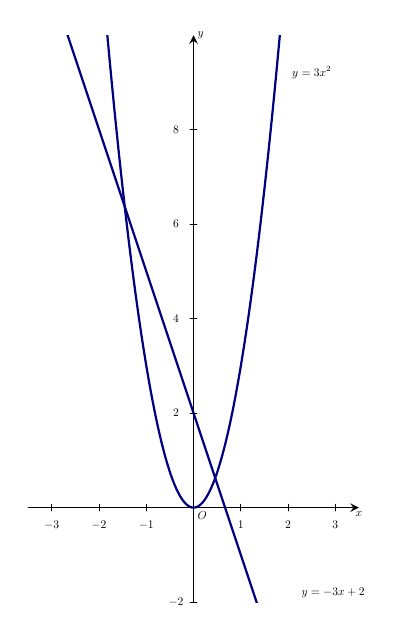
\begin{tikzpicture}[join = round,cap = round,>=stealth,transform shape,scale = 0.6]
		 \def\xmin{-3.5} \def\xmax{3.5}
		 \def\ymin{-2} \def\ymax{10}
		 \def\f (#1){3*(#1)^2}
		\def\g (#1){-3*(#1)+2} 
		\draw[->]  (\xmin,0)--(0,0) node[below right]{$O$}--(\xmax,0) node[below]{$x$};
		\draw[->] (0,\ymin)--(0,\ymax) node[right]{$y$}; 
		\begin{scope}
			\clip (\xmin,\ymin)  rectangle (\xmax,\ymax);
			\draw[smooth,thick,blue!50!black] plot[domain =  \xmin:\xmax,samples = 200,variable=\x]({\x},{\f (\x)}) node[below left] {$y=3x^2$};
			\draw[smooth,thick,blue!50!black] plot[domain = \xmin:\xmax,samples  = 200,variable=\x]({\x},{\g (\x)}) node{$y=-3x+2$};
		\end{scope}
		\foreach \x in  {}{
			\pgfmathsetmacro\fx{\f (\x)} 
			 \draw[dashed,thin] (\x,0) |- (0,{\fx});
		 }
		\foreach \x in {}{ 
			 \pgfmathsetmacro\gx{\g (\x)}
			\draw[dashed,thin] (\x,0)  |- (0,{\gx});
		 }
		\draw (\xmax-1.5,\ymax-1) node [above  right]{$y=3x^2$};
		\draw (\xmax-1.3,\ymin)  node [above right]{$y=-3x+2$};
		 \foreach \x/\g in {-3/-90,-2/-90,-1/-90,1/-90,2/-90,3/-90}
		\draw[thin] (\x,2pt)--(\x,-2pt) + (\g:3mm) node {$\x$}; 
		\foreach  \y/\g in {-2/180,2/180,4/180,6/180,8/180}
		\draw[thin]  (2pt,\y)--(-2pt,\y) + (\g:3mm) node {$\y$};
	\end{tikzpicture}}
	\loigiai{ 
		\begin{itemchoice}
			\itemch \textbf{Sai}. Đồ thị hàm số $y=-3x+2$  là một đường thẳng.
			\itemch \textbf{Đúng}. Đồ thị hàm  số $y=-3x+2$ cắt đồ thị hàm số $y=3x^2$ tại hai điểm.
			\itemch \textbf{Đúng}.Đồ thị của  hàm số $y=-3x+2$ nghịch biến trên $\mathbb{R}$.
			 \itemch \textbf{Sai}. Đồ thị hàm số $y=3x^2$ không nghịch biến trên khoảng $(0;+\infty)$.
		\end{itemchoice}
	 }
\end{ex}

% từ: cau-hoi/lop10/0D3_Ham_so_bac_hai_va_do_thi/0D3-1-4_Do_thi_cua_ham_so.tex
\begin{bt}%[0D3H1-4]\hfill%[ma:42a1deec]
		\begin{enumerate}
			\item \immini{Cho đồ thị của hàm số $y=2x^2$ như sau, dựa vào đồ thị hàm số, hãy tìm $x$ khi $y=8$?}
			{\begin{tikzpicture}[scale=0.8, font=\footnotesize, line join=round, line cap=round, >=stealth]
					\def\a{2}
					\def\b{0}
					\def\c{0}
					\def\f(#1){\a*((#1)^2)+\b*(#1)+\c}
					\def\xmin{-2.5}
					\def\xmax{2.5}
					\def\ymin{-1}
					\def\ymax{4.2}
					\clip (-4,4.2) rectangle (3,-1);
					\draw[->] (\xmin-0.1,0)--(\xmax+0.1,0) node[below] { $x$};
					\draw[->] (0,\ymin-0.1)--(0,\ymax) node[below left] { $y$};
					\draw (0,0) node [below left] { $O$};
					\foreach \x in {-2,-1,1,2}
					\draw (\x,0.1)--(\x,-0.1) node [below] { $\x$};
					\foreach \y in {1,2,3}
					\draw (0.1,\y)--(-0.1,\y) node [left] { $\y$};
					\draw[red,thick,smooth,samples=200] plot[domain=\xmin:\xmax] (\x,{\f(\x)});
					\draw (-3.9,3) node [red,right, sloped] {$(P):y=2x^2$};
			\end{tikzpicture}}
			\item Hãy vẽ đồ thị hàm số $y=2x+1$ và $y=2x^2$ trên cùng một mặt phẳng toạ độ.
		\end{enumerate}
		\loigiai{
			\begin{enumerate}
				\item Khi $y=8$ ta có $2x^2=8$, tức là $x=\pm 2$.\\
				Vậy với $x=\pm 2$ thì $y=8$.
				\item Đồ thị hàm số $y=2x+1$ và $y=2x^2$.
				\begin{center}
					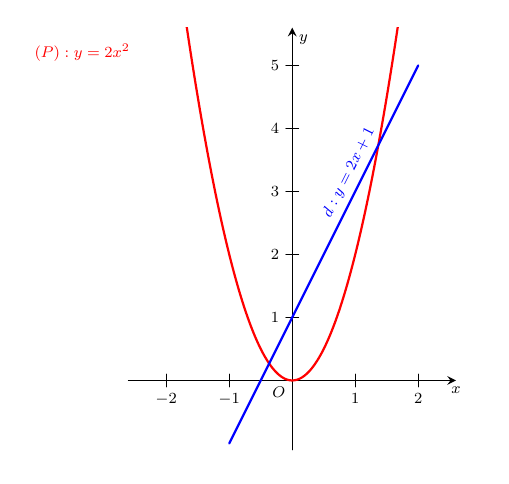
\begin{tikzpicture}[scale=0.8, font=\footnotesize, line join=round, line cap=round, >=stealth]
						\def\a{2}
						\def\b{0}
						\def\c{0}
						\def\f(#1){\a*((#1)^2)+\b*(#1)+\c}
						\def\xmin{-2.5}
						\def\xmax{2.5}
						\def\ymin{-1}
						\def\ymax{4.5}
						\clip (-4.2,5.6) rectangle (3,-1.2);
						\draw[->] (\xmin-0.1,0)--(\xmax+0.1,0) node[below] { $x$};
					\draw[->] (0,\ymin-0.1)--(0,\ymax+1.1) node[below right] { $y$};
						\draw (0,0) node [below left] { $O$};
						\foreach \x in {-2,-1,1,2}
						\draw (\x,0.1)--(\x,-0.1) node [below] { $\x$};
						\foreach \y in {1,2,3,4,5}
						\draw (0.1,\y)--(-0.1,\y) node [left] { $\y$};
						\draw[red,thick,smooth,samples=200] plot[domain=\xmin:\xmax] (\x,{\f(\x)});
						\draw [blue,thick](-1,-1)--(2,5) node [pos=0.7, above, sloped] {$d:y=2x+1$};
						\draw (-4.2,5.2) node [red,right, sloped] {$(P):y=2x^2$};
					\end{tikzpicture}
				\end{center}		
			\end{enumerate}
		}
	\end{bt}

% từ: cau-hoi/lop10/0D3_Ham_so_bac_hai_va_do_thi/0D3-1-4_Do_thi_cua_ham_so.tex
\begin{bt}%[0D3H1-4]%[Mui Doan]%[ma:f13d7cd9]
	Cho hàm số $ y=-2x^2 $.
	\begin{enumerate}
		\item Điểm nào trong các điểm có tọa độ $ (-1;2) $, $ (0;0) $, $ (0;1) $, $ (2~021;1) $ thuộc đồ thị hàm số trên?
		\item Tìm những điểm thuộc đồ thị hàm số có hoành độ lần lượt bằng $ 2 $; $ 3 $ và $ 10 $.
		\item Tìm những điểm thuộc đồ thị hàm số có tung độ  bằng $-18 $.
	\end{enumerate}
	\loigiai{
		\begin{enumerate}
			\item 
			$ x=-1\Rightarrow y=-2(-1)^2=-2 $. Suy ra $ (-1;2) $ không thuộc đồ thị hàm số.\\
			$ x=0\Rightarrow y=-2\cdot 0^2=0 $. Suy ra $ (0;0) $  thuộc đồ thị hàm số; $ (0;1) $ không thuộc đồ thị hàm số.\\
			$ x=2~021\Rightarrow y=-2\cdot 2~021^2\neq 1 $. Suy ra $ (2~021;1) $ không thuộc đồ thị hàm số.
			\item $ x=2\Rightarrow y=-2\cdot 2^2=-8$.\\
			$ x=3\Rightarrow y=-2\cdot 3^2=-18$.\\
			$ x=10\Rightarrow y=-2\cdot 10^2=-200$.\\
			Vậy các điểm thuộc đồ thị hàm số là $ (2;-8) $, $ (3;-18) $, $ (10;-200) $.
			\item $ y=-18\Rightarrow -2x^2=-18\Rightarrow x^2=9\Rightarrow \hoac{&x=3\\&x=-3.}$\\
			Vậy các điểm thuộc đồ thị hàm số là $ (3;-18) $, $ (-3;-18) $.
		\end{enumerate} 
	}
	
\end{bt}

% từ: cau-hoi/lop10/0D3_Ham_so_bac_hai_va_do_thi/0D3-1-5_Tinh_dong_bien_nghich_bien.tex
\begin{ex}%[0D3H1-5]%[ma:c8824602]
	\immini{Cho hàm số $y=f(x)$ xác định trên $\mathbb{R}$ có đồ thị như hình vẽ bên. Mỗi kết  quả dưới đây đúng hay sai?}{
	\begin{tikzpicture}[font=\footnotesize,line join=round,line cap=round,>=stealth,scale=1]
			 \draw[->] (-2,0) -- (3.5,0) node[below] {$x$};
			 \draw[->] (0,-1.2) -- (0,2.5) node[left] {$y$};
			\begin{scope}
				\clip (-2,-1.2) rectangle  (3,2.5);
				 \draw[samples=200,domain=1: 3,smooth,variable=\x] plot (\x,{(\x)-1});
				\draw[samples=200,domain=-2: 1,smooth,variable=\x] plot  (\x,{-1*(\x)+1});
			\end{scope}
			\draw[dashed]  (2,0)--(2,1)--(0,1);
			 \foreach \x/\y in{0/0,1/0,2/0,0/1,2/1,2/0}{
				\fill  (\x,\y) circle (1.5pt);
			} 
			\path 
				node at (0,0)[above left]{$O$} 
				node at  (1,0)[below left]{$1$}
				 node at (2,0)[below]{$2$}
				node at  (0,1)[left]{$1$};
		\end{tikzpicture}
	 }
	\choiceTF 
		{$f(3)=0$} 
		 {\True $f(-2)>f(0)$}
		{Điểm $\left(0;2\right)$ thuộc đồ  thị hàm số}
		 {\True $f(x)=\left|x-1\right|$}
	 \loigiai{
		\begin{itemchoice}
			\itemch Từ  đồ thị $f(3)\ne 0$.
			\itemch Do $f(-2)>f(0)$ vì hàm số  nghịch biến $\left(-\infty;0\right)$.
			\itemch Từ đồ thị của hàm số suy  ra điểm $\left(0;2\right)$ không thuộc đồ thị hàm số.
			\itemch Từ đồ thị  ta có $f(x)=\left|x-1\right|$.
		\end{itemchoice}
	 }
\end{ex}

% từ: cau-hoi/lop10/0D3_Ham_so_bac_hai_va_do_thi/0D3-1-5_Tinh_dong_bien_nghich_bien.tex
\begin{bt}%[0D3H1-5]%[Dự án đề kiểm tra Toán 10 GHKI NH23-24- Huỳnh Quy]%[THPT Tây Thạnh]%[ma:34b2d56d]
	Tìm khoảng đồng biến, nghịch biến của hàm số có đồ thị như hình sau:
	\begin{center}
		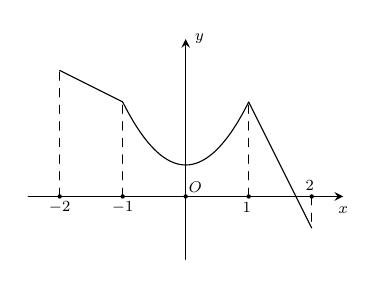
\begin{tikzpicture}[font=\footnotesize,line join=round, line cap=round, >=stealth,scale=0.8] 
			\def \xmin{-2.5}\def \xmax{2.5}\def \ymin{-1}\def \ymax{2.5} 
			\draw[->] (\xmin,0)--(\xmax,0) node[shift=(-90:0.25)] {$x$};
			\draw[->] (0,\ymin)--(0,\ymax) node[shift=(0:0.25)] {$y$};
			\fill (0,0) circle(1pt) node[shift=(45:0.25)]{$O$}
			(1,0) circle(1pt) node[shift=(-100:0.2)]{$1$}
			(2,0) circle(1pt) node[shift=(100:0.2)]{$2$}
			(-2,0) circle(1pt) node[shift=(-90:0.2)]{$-2$}
			(-1,0) circle(1pt) node[shift=(-90:0.2)]{$-1$}
			;
			\draw (-2,2)--(-1,1.5) (1,1.5)--(2,-0.5);
			\begin{scope}
				\clip (\xmin,\ymin) rectangle (\xmax,\ymax); 
				\draw[smooth,samples=100,domain=-1:1] plot(\x,{(\x)^2+0.5});
				%			\draw[smooth,samples=100,domain=\xmin:\xmax] plot(\x,{4-\x});
			\end{scope}
			\draw[dashed] (-2,0)--(-2,2) (-1,0)--(-1,1.5) (1,0)--(1,1.5) (2,0)--(2,-0.5);
		\end{tikzpicture}
	\end{center}
	\loigiai{
		Ta thấy trên các khoảng $(-2;0)$ và $(1;2)$ đồ thị hàm số đi xuống từ trái sang phải nên nghịch biến.\\
		Trên khoảng $(0;1)$, đồ thị hàm số đi lên từ trái sang phải nên hàm số đồng biến.
	}
\end{bt}

% từ: cau-hoi/lop10/0D3_Ham_so_bac_hai_va_do_thi/0D3-1-5_Tinh_dong_bien_nghich_bien.tex
\begin{bt}%[0D3C1-5]%[Dự án Tex Toán 10 chương trình mới]%[ma:111d4ec4]
	Tìm $m$ để hàm số $y=\dfrac{x^2+x+m-5}{x+3}$ đồng biến trên khoảng $(-3;+\infty)$.
	\loigiai{
		Ta có $y= \dfrac{x^2+x+m-5}{x+3} = x-2 + \dfrac{m+1}{x+3}$.\\
		Xét $x_1;x_2 \in (-3;+\infty)$ với $x_1<x_2$, ta có: 
		\begin{eqnarray*}
			y_2-y_1>0 & \Leftrightarrow & x_2-x_1+(m+1)\left( \dfrac{1}{x_2+3}-\dfrac{1}{x_1+3} \right) >0  \\
			&\Leftrightarrow& x_2-x_1+(m+1) \dfrac{x_1-x_2}{(x_1+3)(x_2+3)} >0 \\
			&\Leftrightarrow& (x_2-x_1)\left[ 1-\dfrac{m+1}{(x_1+3)(x_2+3)} \right] >0 \\
			&\Leftrightarrow& \dfrac{(x_1+3)(x_2+3)-m-1}{(x_1+3)(x_2+3)} >0\\
			&\Leftrightarrow& (x_1+3)(x_2+3)>m+1. 
		\end{eqnarray*}
		Để $y_2-y_1>0$ với mọi $x_1,x_2 \in (-3;+\infty)$ thì $m+1 \le 0 \Leftrightarrow m \le -1$.
	}
\end{bt}

% từ: cau-hoi/lop10/0D3_Ham_so_bac_hai_va_do_thi/0D3-2-1_Xac_dinh_ham_so_bac_hai.tex
\begin{ex}%[0D3Y2-1]%[ma:c144145e]
	Tung một đồng xu cân đối và đồng chất một lần. Xác suất của biến cố: \lq\lq Kết quả tung đồng xu được mặt sấp\rq\rq\,  là
	 \choice
		{$\dfrac{1}{3}$} 
		{\True  $\dfrac{1}{2}$}
		 {$\dfrac{3}{4}$}
		{$\dfrac{1}{4}$} 
	\loigiai{ 
		Số  phần tử của không gian mẫu là $2$.\\
		Tung  đồng xu một lần được mặt sấp có $1$ cách.\\
		Suy ra xác suất cần tìm  là $\dfrac{1}{2}$.
	} 
\end{ex}

% từ: cau-hoi/lop10/0D3_Ham_so_bac_hai_va_do_thi/0D3-2-1_Xac_dinh_ham_so_bac_hai.tex
\begin{ex}%[0D3B2-1]%[ma:bde05429]
	Gieo 2 con xúc xắc cân đối và đồng chất. Xác suất để tổng số chấm xuất hiện trên hai mặt của 2 con xúc xắc đó không vượt  quá 4 là?
	 \choice
		{$\dfrac{2}{9}$} 
		 {$\dfrac{5}{18}$}
		{$\dfrac{1}{6}$} 
		 {$\dfrac{2}{3}$}
	 \loigiai{
		Số phần tử không  gian mẫu là $ n\left(\Omega\right)=6\cdot 6=36 $.\\
		Gọi $ A $ là biến cố ~\lq\lq tổng số chấm xuất hiện  trên hai mặt của $ 2 $ con xúc sắc không vượt quá 4.\rq\rq\\
		Suy ra  $ A=\{(1,1);(1,2);(1,3);(2,1);(2;2);(3,1)\} $.\\
		Do  đó $ n(A)=5 $.\\
		Xác suất cần tìm là $  P=\dfrac{1}{6} $.
	 }
\end{ex}

% từ: cau-hoi/lop10/0D3_Ham_so_bac_hai_va_do_thi/0D3-2-3_Do_thi_cua_ham_so_bac_hai.tex
\begin{ex}%[0D3B2-3]%[ma:ff4f8bd5]
	Một tổ trong lớp 10A có $4$ bạn nam và $6$ bạn nữ. Giáo viên chọn ngẫu nhiên hai bạn trong tổ để tham gia đội làm báo của  lớp. Xác suất để hai bạn được chọn có một bạn nam và một bạn nữ là?
	\choice 
		 {$\dfrac{2}{15}$}
		{$\dfrac{6}{25}$} 
		{$\dfrac{8}{25}$} 
		 {\True $\dfrac{8}{15}$}
	 \loigiai{
		Ta có $n(\Omega)=\mathrm{C}_{10}^2=45$.\\ 
		Biến cố $A$ \lq\lq Hai  bạn được chọn có một bạn nam và một bạn nữ\rq\rq.\\
		Suy  ra, $n(A)=\mathrm{C}_6^1\cdot\mathrm{C}_4^1=24$.\\
		Vậy xác suất biến cố $A$ là $\mathrm{P}(A)=\dfrac{n(A)}{n(\Omega)}=\dfrac{24}{45}=\dfrac{8}{15}$. 
	} 
\end{ex}

% từ: cau-hoi/lop10/0D3_Ham_so_bac_hai_va_do_thi/0D3-2-4_Bai_toan_ve_su_tuong_giao.tex
\begin{ex}%[0D3B2-4]%[ma:9bb4454d]
	Một  hộp đựng $ 12 $ bóng đèn trong đó có $ 4 $ bóng hỏng. Chọn ngẫu nhiên $ 3 $ bóng. Xác suất của biến cố $A\colon$ \lq\lq \textbf{Không} có bóng đèn nào hỏng\rq\rq~ là?
	 \choice
		{$\dfrac{28}{55}$} 
		 {$\dfrac{8}{55}$}
		{$\dfrac{7}{55}$} 
		 {\True $\dfrac{14}{55}$}
	 \loigiai{
		Số phần tử không gian mẫu là $  n(\Omega) =\mathrm{C}^3_{12}=220$.\\
		Số cách chọn ra ba bóng  không có bóng hỏng là $ n(A)=\mathrm{C}^3_{8}=56$.\\
		Xác suất cần tìm  là $ P(A)=\dfrac{14}{55} $.
	 }
\end{ex}

% từ: cau-hoi/lop10/0D3_Ham_so_bac_hai_va_do_thi/0D3-2-4_Bai_toan_ve_su_tuong_giao.tex
\begin{ex}%[0D3B2-4]%[ma:89fd4578]
	Một hộp có $5$ bi  đen, $4$ bi trắng. Chọn ngẫu nhiên $2$ bi. Xác suất $2$ bi được chọn có đủ hai màu là
	\choice 
		{\True $\dfrac{5}{9}$} 
		 {$\dfrac{2}{9}$}
		 {$\dfrac{5}{214}$}
		{$\dfrac{1}{18}$} 
	\loigiai{ 
		Chọn ngẫu nhiên $2$ bi từ hộp có $5$ bi đen, $4$ bi trắng, có $n(\Omega)=\mathrm{C}_9^2=36$ kết  quả có thể xảy ra.\\
		Biến cố  $A\colon$ ``$2$ bi được chọn có đủ $2$ màu'' có $n(A)=5\cdot 4=20$.\\
		 Vậy xác suất của $A$ là $\mathrm{P}(A)=\dfrac{n(A)}{n(\Omega)}=\dfrac{20}{36}=\dfrac{5}{9}$.
	} 
\end{ex}

% từ: cau-hoi/lop10/0D3_Ham_so_bac_hai_va_do_thi/0D3-2-4_Bai_toan_ve_su_tuong_giao.tex
\begin{bt}%[0D3B2-4]%[ma:6f9f07b9]
	 (1.0 điểm)
	Một hộp đựng $ 7 $ bi xanh  và $ 6 $ bi đỏ. Chọn ngẫu nhiên $ 5 $ viên bi. Tính xác suất để $ 5 $ bi được chọn có đủ hai màu và số bi xanh nhiều hơn số bi đỏ.
	 \loigiai{
		Số  phần tử của không gian mẫu là $ n(\Omega) =\mathrm{C}^5_{13}= 1287$.\\
		Gọi $ A $ là biến cố~ \lq\lq $ 5 $ bi được chọn có đủ hai màu và số bi  xanh nhiều hơn số bi đỏ\rq\rq.\\
		Để chọn $ 5 $ bi được chọn có đủ hai màu và số bi xanh nhiều  hơn số bi đỏ ta có các trường hợp sau
		\begin{itemize}
			\item  [\bf TH1:] $ 3 $ xanh và $ 2 $ đỏ có $ \mathrm{C}^3_7 \cdot\mathrm{C}^2_6 =525$.
			\item [\bf TH2:]  $ 4 $ xanh và $ 1 $ đỏ có $ \mathrm{C}^4_7 \cdot\mathrm{C}^1_6 =210$.
		\end{itemize}
		Suy ra $ n\left(A\right)=735  $.\\
		 Xác suất cần tìm là $ P(A)= \dfrac{245}{429}$.
	 }
\end{bt}

% từ: cau-hoi/lop10/0D3_Ham_so_bac_hai_va_do_thi/0D3-2-6_Toan_thuc_te_ung_dung_ham_so_bac_hai.tex
\begin{ex}%[0D3B2-6]%[ma:ecd46391]
	Từ các chữ số $1$; $2$; $4$; $6$; $8$; $9$  lấy ngẫu nhiên một số. Xác suất để lấy được một số nguyên tố là
	\choice 
		{$\dfrac{1}{2}$} 
		{$\dfrac{1}{3}$} 
		{$\dfrac{1}{4}$} 
		 {\True $\dfrac{1}{6}$}
	 \loigiai{
		 Ta có $n(\Omega)=6$.\\
		Biến cố $A$ \lq\lq Lấy được một  số nguyên tố\rq\rq.\\
		 $A=\left\{2\right\}$, suy ra $n(A)=1$.\\
		Vậy xác suất biến cố $A$ là $\mathrm{P}(A)=\dfrac{n(A)}{n(\Omega)}=\dfrac{1}{6}$. 
	} 
\end{ex}

% từ: cau-hoi/lop10/0D3_Ham_so_bac_hai_va_do_thi/0D3-2-6_Toan_thuc_te_ung_dung_ham_so_bac_hai.tex
\begin{ex}%[0D3B2-6]%[ma:125bdab4]
	Cho tập hợp $A=\{0;1;2;3;4;5;6\}$ và $S$ là tập hợp các số tự nhiên có ba chữ số khác nhau được lập từ các chữ số của tập hợp $A$. Lấy ngẫu nhiên một số thuộc tập hợp $S$. Xác suất của biến cố: "Số được  chọn là một số chia hết cho $5$" là
	\choice 
		{$\dfrac{11}{35}$} 
		{$\dfrac{11}{42}$} 
		{\True $\dfrac{11}{36}$} 
		{$\dfrac{11}{24}$} 
	 \loigiai{
		Gọi số cần tìm trong tập $S$  có dạng $\overline{abc}$.\\
		 Ta có
		\begin{itemize}
			\item Chọn $a\in  A\setminus\{0\}$ có $6$ cách.
			\item Chọn $b\in A\setminus\{a\}$  có $6$ cách.
			\item Chọn  $c\in A\setminus\{a;b\}$ có $5$ cách.
		\end{itemize}
		Do đó tập $S$ có $6\cdot 6\cdot  5=180$ phần tử.\\
		Suy ra số phần tử của không gian mẫu là  $n(\Omega)=\mathrm{C}_{180}^1=180$.\\
		Gọi $X$ là biến cố \lq\lq Số được chọn là một số  chia hết cho $5$\rq\rq.\\
		Khi đó ta  có
		\begin{itemize}
			\item \textbf{TH1.} $c=0$.\\ 
			Số cách  chọn $\overline{ab}$ là $\mathrm{A}_{6}^2=30$ cách.\\
			Suy  ra trường hợp này có $30$ số chia hết cho $5$.
			\item  \textbf{TH2.} $c=5$.
			\begin{itemize}
				\item Chọn $a\in A\setminus\{0\}$ có $5$  cách.
				\item Chọn $b\in A\setminus\{a,  c\}$ có $5$ cách.
			\end{itemize}
			Suy ra trường hợp này có $5\cdot5=25$ số chia hết cho $5$. 
		\end{itemize}
		 Do đó số phần tử của biến cố $X$ là $n(X)=30+25=55$.\\
		Vậy xác suất cần  tính là $\mathrm{P}(X)=\dfrac{n(X)}{n(\Omega)}=\dfrac{55}{180}=\dfrac{11}{36}$.
	} 
\end{ex}

% từ: cau-hoi/lop10/0D7_Bat_phuong_trinh_bac_2_mot_an/0D7-1-2_Dau_cua_tam_thuc_bac_2_va_ung_dung.tex
\begin{bt}%[0D7V1-2]%[ma:88e2cc65]
	Tính tổng bình phương các  giá trị nguyên của tham số $ m $ để bất phương trình $ (m-1)x^2+2(m-1)x+5<0 $ vô nghiệm.
	\shortans{91} 
	\loigiai{ 
		Bất phương trình $ (m-1)x^2+2(m-1)x+5<0 $ vô nghiệm  khi và chỉ khi $ (m-1)x^2+2(m-1)x+5\geq 0 $, $ \forall x\in \mathbb{R} $. \hfill(1)\\
		{\bf Trường hợp 1.} Nếu $ m= 1 $  thì $ (1)\Leftrightarrow 5\geq 0 $, $ \forall x\in \mathbb{R} $. Điều này luôn đúng nên nhận $ m=1 $.\\
		{\bf Trường hợp 2.}  Nếu $ m\neq 1 $ thì
		\[(1)\Leftrightarrow \heva{&m-1>0\\&\Delta'=(m-1)^2-5(m-1)\leq  0}\Leftrightarrow \heva{&m>1\\&m^2-7m+6\leq 0}\Leftrightarrow \heva{&m>1\\&1\leq m\leq 6}\Leftrightarrow 1<m\leq 6.\]
		Vì $ m $ nguyên  nên $ m\in \{2;3;4;5;6\} $.\\
		Vậy có tất cả $ 6 $ giá trị của $ m  $ thỏa mãn. Tổng bình phương các giá trị đó là $91$.
	} 
\end{bt}

% từ: cau-hoi/lop10/0D7_Bat_phuong_trinh_bac_2_mot_an/0D7-1-3_Bai_toan_xet_dau_biet_BXD_do_thi.tex
\begin{bt}%[0D7H1-3]%[Dự án đề kiểm tra GHKII NH22-23- Dương Phước Sang]%[Marie Curie]%[ma:0e08e306]
		\immini{
			Cho hàm số $f(x)=ax^2+bx+c$ có đồ thị $(C)$ như hình vẽ.
			\begin{enumerate}
				\item Từ đồ thị hãy xác định dấu của hệ số $a$ và $\Delta $. 
				\item Tìm tập nghiệm của bất phương trình $f(x)<0$.
			\end{enumerate}}
		{\vspace{-0.5cm}
			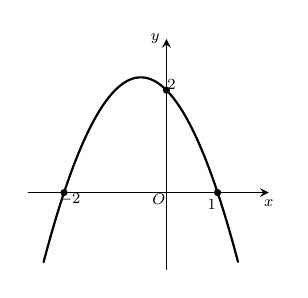
\begin{tikzpicture}[line join=round, line cap=round,>=stealth,font=\footnotesize,scale=0.65]
				\draw[->] (-2.7,0)--(2,0) node[below ] {$x$};
				\draw[->] (0,-1.5)--(0,3) node[left] {$y$};
				\draw (0,0) node [below left=-3pt] {$O$} (1,0) node [below,xshift=-3] {$1$} (-2,0) node [below right=-3pt,xshift=-3] {$-2$} (0,2) node [above right=-3pt] {$2$};
				;
				\fill (1,0) circle (2pt);
				\fill (-2,0) circle (2pt);
				\fill (0,2) circle (2pt);
				\foreach \x in {}
				\draw[thin] (\x,1pt)--(\x,-1pt) node [below] {$\x$};
				\foreach \y in {}
				\draw[thin] (1pt,\y)--(-1pt,\y) node [left] {$\y$};
				\draw[thick,samples=200,domain=-2.4:1.4,smooth,variable=\x] plot (\x,{-1*(\x)^2-1*(\x)+2});
				
		\end{tikzpicture}	}
		\loigiai{
			\begin{enumerate}
				\item Do đồ thị là parabol có bề lõm quay xuống nên $a<0$.\\
				Ngoài ra đồ thị hàm số cắt trục $ Ox $ tại hai điểm phân biệt nên $\Delta >0$.\\
				Như vậy $\heva{&a<0\\&\Delta>0.}$
				\item Dựa vào đồ thị, ta thấy $ f(x)<0 \Leftrightarrow x \in (-\infty;-2) \cup (1;+\infty)$.\\ 
				Vậy bất phương trình $f(x)<0$ có tập nghiệm $S=(-\infty;-2) \cup (1;+\infty)$.
				
			\end{enumerate}
			
		}
	\end{bt}

% từ: cau-hoi/lop10/0D7_Bat_phuong_trinh_bac_2_mot_an/0D7-1-4_Xet_dau_bieu_thuc_dang_tich_thuong.tex
\begin{ex}%[0D7H1-4]%[ma:da13e1f7]
	Gọi $ S $ là tập nghiệm của bất phương trình  $\dfrac{x^2 - 2x + 1}{x^2 - 9} \geq 0.$
	Khi đó $S\cap (-3;3) $  là tập nào sau đây?
	\choice 
		{$(-3;1]$} 
		 {$(-3;3)$}
		{$(-3;0)$} 
		{\True $\{1\}$} 
	 \loigiai{
		Ta có tử số $x^2 - 2x +  1= (x-1)^2 $ luôn không âm và bằng 0 khi $ x = 1 $.\\
		 Từ bất phương trình $f(x)=\dfrac{(x-1)^2}{(x-3)(x+3)} \geq 0$. Ta có bảng xét dấu
		\begin{center}
			
\begin{tikzpicture}
					\tikzset{t  style/.style={style=draw}}
					 \tkzTabInit[deltacl=0.5,espcl=2.5,lgt=2,nocadre]
						 {$x$/1,$(x-1)^2$/1,$(x-3)$/1,$(x+3)$/1,$f (x)$/1}
						{$8$,$-3$,$1$,$3$,$8$} 
					 \tkzTabLine{,+,,+,0,+,,+,}
					\tkzTabLine{,-,,-,,-,0,+,} 
					\tkzTabLine{,-,0,+,,+,,+,} 
					 \tkzTabLine{,+,||,-,0,-,||,+,}
				\end{tikzpicture}
		\end{center}
		$\Rightarrow S=\left(-\infty;  -3\right)\cup \left(3;+\infty\right)\cup \{1\}$.\\
		Vậy $ S \cap (-3;3) = \{1\}  $.
	} 
\end{ex}

% từ: cau-hoi/lop10/0D7_Bat_phuong_trinh_bac_2_mot_an/0D7-2-2_Giai_bat_phuong_trinh_bac_hai_biet_BXD_do_thi.tex
\begin{ex}%[0D7H2-2]%[ma:02870b30]
	 \immini
	 {
	Cho hàm số bậc hai $f(x)=ax^2+bx+c$ có đồ thị  như hình vẽ bên.
	\choiceTF 
		{\True  $a>0$}
		 {$f(0)=1$}
		{Phương trình $f(x)=0$ có hai  nghiệm trái dấu}
		{\True Tập nghiệm của bất  phương trình là $f(x)>0$ là $(-\infty;1)\cup(2;+\infty)$}
		 }
		{ 
		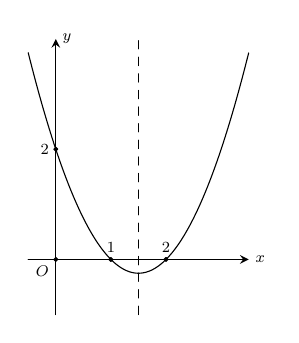
\begin{tikzpicture}[line cap=round,line join=round,>=stealth,font=\footnotesize,scale=0.7]
				\def\xmin{-.5} 
				\def\xmax{3.5} 
				 \def\ymin{-1}
				\def\ymax{4} 
				\draw[-stealth] (\xmin,0)--(\xmax,0)  node[right]{$x$};
				 \draw[-stealth] (0,\ymin)--(0,\ymax) node[right]{$y$};
				 \draw[samples=200,domain=\xmin:\xmax]plot (\x,{(\x)^2-3*(\x)+2});
				\draw[fill=black] (0,0) circle (1pt) node[below  left]{$O$};
				\draw[dashed]  (1.5,\ymin)--(1.5,\ymax);
				\clip (\xmin,\ymin)  rectangle (\xmax,\ymax);
				 \fill[draw] (1,0) node[above]{$1$} circle (1pt);
				\fill[draw]  (2,0) node[above]{$2$} circle (1pt);
				\fill[draw] (0,2)  node[left]{$2$} circle (1pt);
			\end{tikzpicture}
		} 
	\loigiai{ 
		\begin{itemchoice}
			 \itemch Từ đồ thị hàm số $f(x)$ ta thấy bề lõm hướng lên nên suy ra $a>0$.
			\itemch Từ  đồ thị hàm số $f(x)$ ta có $f(0)=2$.
			\itemch Từ đồ thị hàm số $f(x)$  ta có $f(x)=0 \Leftrightarrow \hoac{&x=1>0\\&x=2>0.}$
			\itemch Từ đồ thị hàm số $f(x)$ ta có  bảng xét dấu
			\begin{center}
				
\begin{tikzpicture}
					 \tkzTabInit[lgt=1.2,espcl=2.5,deltacl=0.6]
						 {$x$/0.6,$f (x)$/0.6}{$-\infty$,$1$,$2$,$+\infty$}
					\tkzTabLine{,+,0,-,0,+,} 
				\end{tikzpicture}
			\end{center}
			Tập nghiệm của bất phương trình $f(x)>0$  là $S=(-\infty;1)\cup(2;+\infty)$.
		\end{itemchoice}
	} 
\end{ex}

% từ: cau-hoi/lop10/0D7_Bat_phuong_trinh_bac_2_mot_an/0D7-2-2_Giai_bat_phuong_trinh_bac_hai_biet_BXD_do_thi.tex
\begin{bt}%[0D7H2-2]%[GHKII-2022-2023-TRƯỜNG THPT NGUYỄN HỮU HUÂN-Thehung Nguyen]%[ma:33dea336]
	 Cho đồ thị của hàm số bậc hai $f(x)$ bên dưới. Tìm tập nghiệm của bất phương trình tương ứng.
	 \begin{center}
	 	\begin{tikzpicture}[>=stealth,line join=round,line cap=round,font=\footnotesize,scale=1]
	 		\draw[->] (-2.5,0)--(1.7,0)node[above right]{$x$};
	 		\draw[->] (0,-2.5)--(0,1)node[left]{$y$};
	 		\fill (0,0)node[below left]{ $O$};
	 		\draw[black,samples=150,smooth,domain=-2.2:1.2] plot(\x,{(\x)^2+(\x)-2});
	 		\draw (-2,0)node[below left]{$-2$} (1,0)node[below right]{$1$}
	 		(-0.5,-3)node {$\mathrm{a})\,f(x) \geq 0.$}
	 		;
	 	\end{tikzpicture}
 		\begin{tikzpicture}[>=stealth,line join=round,line cap=round,font=\footnotesize,scale=1]
 		\draw[->] (-.5,0)--(4,0)node[above right]{$x$};
 		\draw[->] (0,-2.5)--(0,1)node[left]{$y$};
 		\fill (0,0)node[below left]{ $O$};
 		\draw[black,samples=150,smooth,domain=.45:3.5] plot(\x,{-1*(\x)^2+4*(\x)-4});
 		\draw (2,0)node[above]{$2$}
 		(2,-3)node {$\mathrm{b})\,f(x)<0.$}
 		;
 	\end{tikzpicture}
	 \end{center}
	 
\loigiai{
	\begin{enumerate}
		\item Dựa vào đồ thị $f(x) \geq 0\Leftrightarrow\hoac{&x\le -2\\&x\ge 1.}$\\
		Vậy $S=(-\infty;-2]\cup[1;+\infty)$ là tập nghiệm của bất phương trình.
		\item Dựa vào đồ thị $f(x)<0\Leftrightarrow x\neq 2$.\\
		Vậy $S=\mathbb{R}\setminus\{2\}$ là tập nghiệm của bất phương trình.
	\end{enumerate}
}
\end{bt}

% từ: cau-hoi/lop10/0D7_Bat_phuong_trinh_bac_2_mot_an/0D7-2-2_Giai_bat_phuong_trinh_bac_hai_biet_BXD_do_thi.tex
\begin{bt}%[0D7N2-2]%[Dự án đề kiểm tra HKII NH22-23- Nguyễn Văn Sang]%[THPT TRẦN QUANG KHẢI]%[ma:4e57c264]
	\immini
	{
	Dựa vào đồ thị của hàm số trong hình vẽ, hãy xác định nghiệm của bất phương trình $f(x) \leq 0$.
	}
	{
	\begin{tikzpicture}[>=stealth,x=1cm,y=1cm,scale=.75]
		\draw[->] (-4,0) -- (2,0) node[below] {$x$};
		\draw[->] (0,-3.5) -- (0,3) node[left] { $y$};
		\fill (0,0)circle (1.5pt) node[below left]{ $O$};
		\fill (-3,0)circle (1.5pt) node[below left]{$-3$};
		\fill (0.5,0)circle (1.5pt) node[below right]{$0.5$};
		\draw (-2.75,2)node[above]{$f(x)$};
		\draw[samples=150,smooth,domain=-3.5:1] plot(\x,{(\x)^2+2.5*\x-1.5});
	\end{tikzpicture}
	}
	\loigiai{
	Dựa vào đồ thị hàm số $y=f(x)$ ta có bảng xét dấu như sau
\begin{center}
	
\begin{tikzpicture}
		\tkzTabInit[lgt=2,espcl=2,deltacl=0.5]
		{$x$/1 ,$f(x)$/1}
		{$-\infty$ , $-3$ , $\dfrac{1}{2}$, $+\infty$}
		\tkzTabLine{,+,0,-,0,+,}
	\end{tikzpicture}
\end{center}
Ta được $f(x)\leq 0$ với mọi $x\in \left[-3;-\dfrac{1}{2}\right] $.\\
Vậy tập nghiệm của bất phương trình là $S=\left[-3;\dfrac{1}{2}\right]$.
	}
\end{bt}

% từ: cau-hoi/lop10/0D7_Bat_phuong_trinh_bac_2_mot_an/0D7-3-1_Phuong_trinh_can.tex
\begin{ex}%[0D7N3-1]%[ma:b73a4271]
	Phương trình tổng quát của đường thẳng đi qua  $M(-3; 1)$ và có vectơ pháp tuyến $\overrightarrow{n}=(2; 3)$ là
	\choice 
		 {\True $2x+3y+3=0$}
		 {$2x+3y+5=0$}
		{$3x+2y-9=0$} 
		{$-3x+y+2=0$} 
	\loigiai{ 
		Phương trình của đường thẳng đi qua  $M(-3; 1)$ và có vectơ pháp tuyến $\overrightarrow{n}=(2; 3)$ là\\
		\centerline{$2(x+3)+3(y-1)=0  \Leftrightarrow 2x+3y+3=0$.}
	} 
\end{ex}

% từ: cau-hoi/lop10/0D7_Bat_phuong_trinh_bac_2_mot_an/0D7-3-2_Phuong_trinh_can.tex
\begin{bt}%[0D7K3-2]%[ma:c5c56730]
	Cho tam giác $ABC$ vuông tại $A$ có $AB$ ngắn hơn  $AC$ là $2\,\mathrm{cm}$, đặt $A B=x\, \mathrm{cm} $.
	\begin{listEX}
		\item Biểu diễn độ dài cạnh huyền  $BC$ theo $x$.
		\item Biết chu vi của tam giác $ABC$  là $24\,\mathrm{cm}$. Tìm độ dài $3$ cạnh của tam giác đó.
	\end{listEX}
	\loigiai{ 
		\begin{listEX}
			\item Gọi $A B=x \Rightarrow A C=x+2$.\\ 
			 Ta có tam giác $ABC$ vuông tại $A$ nên
			\allowdisplaybreaks{ 
			\begin{eqnarray*}
				&& BC^2 =  AB^2+AC^2 \\
				&\Leftrightarrow& BC^2 =  x^2+(x+2)^2 \\
				&\Rightarrow&  BC = \sqrt{2x^2+4x+4}.
			\end{eqnarray*}
			} 
			\item Ta có chu vi tam giác $ABC$ bằng  $24$ nên
			 \allowdisplaybreaks{
			\begin{eqnarray*}
				&&  A B+A C+B C=24\\
				&\Leftrightarrow& x+x+2+\sqrt{2x^2+4x+4}=24\\ 
				&\Leftrightarrow&  \sqrt{2x^2+4x+4}=22-2x\\
				&\Leftrightarrow& -2 x^2+92 x-480=0\\ 
				 &\Leftrightarrow& \hoac{&x=6 \\&x=40.}
			\end{eqnarray*}
			} 
			Thử lại, nhận $x=6$, loại  $x=40$.\\
			 Vậy độ dài ba cạnh là $AB=6$ cm, $AC=8$ cm và $B C=10$ cm.
		\end{listEX}
	} 
\end{bt}

% từ: cau-hoi/lop10/0D7_Bat_phuong_trinh_bac_2_mot_an/0D7-3-6_Toan_hinh_toan_thuc_te_ung_dung_phuong_trinh.tex
\begin{bt}%[0D7C3-6]%[ma:83493e8d]
	 \immini{
	Một đài quan sát $O$ cách ba vị trí $A$, $B$, $C$ như hình vẽ dưới đây thoả mãn $OB = x$ km, $OC = x+1$ km và $OA = 2$ km. Tìm $x$ biết khoảng cách từ vị trí $A$ đến vị trí $C$ gấp đôi khoảng cách từ vị trí $A$ đến vị trí $B$ và khoảng cách từ $O$ đến $B$ ngắn hơn khoảng cách  từ $O$ đến $A$.
	 }{
	\begin{tikzpicture}[line join = round,line cap = round,scale=.8]
			\coordinate[label = left:$B$] (B)  at (0,0);
			 \coordinate[label = right:$C$] (C) at ($(B)+(6,0)$);
			\coordinate[label = above:$A$] (A)  at ($(B)+(0,4)$);
			\coordinate[label = below:$O$] (O)  at ($(B)+(2,0)$);
			\draw[fill  = gray!50] ($(B)!5pt!(C)$)--($(B)!5pt!(C)+(B)!5pt!(A)-(B)$)--($(B)!5pt!(A)$)--(B)--cycle;
			\draw (B)--(C)--(A)--cycle  (A)--(O);
			\foreach \x in {B,C,A,O} \fill[black] (\x) circle (1pt); 
			\draw pic[draw,black,angle radius=3mm] {angle  = C--O--A}
				($($(O)!18mm!(C)$)!.6!($(O)!13mm!(A)$)$) node[rotate=0]{$120^\circ$}; 
		\end{tikzpicture}
	 }
	\shortans{1} 
	 \loigiai{
		Áp dụng định lý cosintrong  tam giác $AOC$ ta được
		 \[
		AC^2=AO^2+OC^2-2\cdot AO\cdot OC \cdot\cos\widehat{AOC}=4+(x+1)^2-4(x+1)\cdot\cos120^\circ=x^2+4x+7. 
		\] 
		Suy ra  $AC=\sqrt{x^2+4x+7}$.\\
		Áp dụng định lý  cosintrong tam giác $AOB$ ta được
		\[ 
		AB^2=AO^2+OB^2-2\cdot AO\cdot  OB\cos\widehat{AOB}=4+x^2-4x\cos60^\circ=x^2-2x+4.
		\] 
		Suy ra  $AB=\sqrt{x^2-2x+4}$.\\
		Theo giả  thiết ta có $AC=2BO \Leftrightarrow 2\sqrt{x^2-2x+4}=\sqrt{x^2+4x+7}.\quad (*)$\\
		Giải  phương trình $2\sqrt{x^2-2x+4}=\sqrt{x^2+4x+7}.\quad(*)$\\
		Bình phương hai vế của phương trình $(*)$ ta được  phương trình $4(x^2-2x+4)=x^2+4x+7$. \\
		Ta có $$4(x^2-2x+4)=x^2+4x+7 \Leftrightarrow 3x^2-12x+9=0  \Leftrightarrow
		 \hoac{& x=1\\&x=3.}$$
		Thay hai giá trị $x=1$ và $x=3$ vào phương trình $(*)$ ta thấy cả hai giá trị đều thõa  mãn, nhưng $OB<OA$ nên $x=1$.
	 }
\end{bt}

% từ: cau-hoi/lop10/0D7_Bat_phuong_trinh_bac_2_mot_an/0D7-3-6_Toan_hinh_toan_thuc_te_ung_dung_phuong_trinh.tex
\begin{bt}%[0D7V3-6]%[Dự án đề kiểm tra HKII NH22-23- Nguyễn Cường]%[THPT Gia Định]%[ma:04939db6]
	Cho tam giác $ABC$ vuông tại $A$, độ dài cạnh huyền $BC$ lớn hơn độ dài cạnh $AC$ là $2$ (cm). Tính độ dài các cạnh của $\triangle ABC$, biết chu vi $\triangle ABC$ là $24$ (cm).
	\loigiai{
\immini{
Đặt $AC=x$ (cm) với $x>0$, ta có
\begin{itemize}
	\item $BC=x+2$.
	\item Áp dụng định lý Pi-ta-go, ta có
	\[AB=\sqrt{BC^2-AC^2}=\sqrt{(x+2)^2-x^2}=\sqrt{4x+4}. \]
\end{itemize}
}{
\begin{tikzpicture}[>=stealth,line join=round,line cap=round,font=\footnotesize,scale=1]
	\def\r{2};
	\def\g{110};
	\path
	(0,0) coordinate (O)
	(0:\r) coordinate (C)
	(180:\r) coordinate (B)
	(\g:\r) coordinate (A)
	;
	\draw
	(A)--(B)--(C)--cycle
	;
	\foreach \x/\g in {B/180,C/0,A/130}\fill[black](\x) circle (1pt) +(\g:3mm) node {$\x$};
	\foreach \x/\y/\z in {B/A/C}{\draw pic[draw,angle radius=2mm]{right angle=\x--\y--\z};}
\end{tikzpicture}
}	
\noindent Do chu vi $\triangle ABC$ là $24$ (cm) nên 
\allowdisplaybreaks
\begin{eqnarray*}
	x+x+2+\sqrt{4x+4}=24&\Leftrightarrow& 2x+2+2\sqrt{x+1}=24\\
	&\Leftrightarrow&x+1+\sqrt{x+1}=12\\
	&\Leftrightarrow& \sqrt{x+1}=11-x \quad \quad (1)\\
	&\Rightarrow&x+1=(11-x)^2\\
	&\Leftrightarrow&x^2-23x+120=0\\
	&\Leftrightarrow&\hoac{&x=8\\&x=15.}
\end{eqnarray*}
Với $x=15$ thử lại phương trình (1), ta có $\sqrt{16}\ne -4$, nên $x=15$ không là nghiệm.\\
Với $x=8$ thử lại phương trình (1), ta có $\sqrt{16}=4$, nên $x=8$ là nghiệm của phương trình.\\
Vậy độ dài ba cạnh của $\triangle ABC$ là $AC=8$ cm, $BC=10$ cm và $AB=6$ cm.
	}
\end{bt}

% từ: cau-hoi/lop10/0D8_Dai_so_to_hop/0D8-2-6_Bai_toan_co_yeu_to_hinh_hoc.tex
\begin{ex}%[0D8N2-6]%[ma:b4a1849d]
	Trên mặt phẳng cho lục giác $ABCDEF$. Hỏi có  bao nhiêu véc-tơ khác véc-tơ $\overrightarrow 0 $ và có điểm đầu, điểm cuối là 2 trong 6 đỉnh của lục giác đã cho?
	\choice 
		{$36$} 
		 {\True $30$}
		{$11$} 
		{$25$} 
	 \loigiai{
	Mỗi véc-tơ tạo thành là một chỉnh hợp chập $2$ của $6$ phần tử.\\ 
	Vậy số véc-tơ thoả mãn bài toán là $\mathrm{A}_6^2=  30$.
	} 
\end{ex}

% từ: cau-hoi/lop10/0D8_Dai_so_to_hop/0D8-2-6_Bai_toan_co_yeu_to_hinh_hoc.tex
\begin{ex}%[0D8H2-6]%[ma:bce5672c]
	Cho $n$ điểm phân biệt. Xét tất cả các véc-tơ  khác $\overrightarrow{0}$, có điểm đầu và điểm cuối là các điểm đã cho. Số véc-tơ thoả mãn là
	 \choice
		 {$n$}
		{$n-1$} 
		{$\dfrac{n(n-1)}{2}$} 
		 {\True $n(n-1)$}
	\loigiai{ 
		Mỗi véc-tơ khác $\overrightarrow{0}$  là một chỉnh hợp chập $2$ của $n$ điểm đã cho.\\
		Vậy số véc-tơ thoả  mãn bài toán là $\mathrm{A}_n^2=n(n-1)$.
	} 
\end{ex}

% từ: cau-hoi/lop10/0D8_Dai_so_to_hop/0D8-3-2_Khai_trien_mot_nhi_thuc_Newton.tex
\begin{ex}%[0D8H3-2]%[ma:8a2c52a8]
	Kết  quả của khai triển $(x-y)^4$ là
	 \choice
		{\True $x^4-4x^3y+6x^2y^2-4xy^3+y^4$} 
		{$x^4-x^3y+x^2y^2-xy^3+y^4$} 
		 {$x^4-4x^3y+12x^2y^2-24xy^3+24y^4$}
		 {$x^4+4x^3y+6x^2y^2+4xy^3+y^4$}
	 \loigiai{
		Dựa vào tam giác Pascal hoặc công thức khai triển nhị  thức Niu-tơn ta có ngay
		 \[(x-y)^4=x^4-4x^3y+6x^2y^2-4xy^3+y^4.\]
	 }
\end{ex}

% từ: cau-hoi/lop10/0D8_Dai_so_to_hop/0D8-3-5_Tinh_tong_nho_khai_trien_nhi_thuc_Newton.tex
\begin{bt}%[0D8V3-5]%[ma:ba23ea5e]
	Rút gọn biểu thức $S=\dfrac{1}{1\cdot 0!\cdot 2019!}+\dfrac{1}{2\cdot 1!\cdot  2018!}+\dfrac{1}{3\cdot 2!\cdot 2017!}+\cdots+\dfrac{1}{2020\cdot 2019!\cdot 0!}$.
	 \loigiai{
		Ta có  $S=\displaystyle\sum\limits_{k=0}^{2019} \dfrac{1}{(k+1) k!(2019-k)!}=\displaystyle\sum\limits_{k=0}^{2019} \dfrac{2020!}{2020!(k+1)!(2020-(k+1))!}=\dfrac{1}{2020!} \displaystyle\sum\limits_{k=0}^{2019} \mathrm{C}_{2020}^{k+1}$.\\
		Xét khai triển $(x+1)^{2020}=\displaystyle\sum\limits_{k=0}^{2020} \mathrm{C}_{2020}^k \cdot x^k=1+\displaystyle\sum\limits_{k=1}^{2020} \mathrm{C}_{2020}^k \cdot x^k$.\\ 
		Chọn $x=1$ ta thu được $\displaystyle\sum\limits_{k=1}^{2020} \mathrm{C}_{2020}^k=\displaystyle\sum\limits_{k=0}^{2019}  \mathrm{C}_{2020}^{k+1}=2^{2020}-1$.\\
		 Vậy $S=\dfrac{2^{2020}-1}{2020!}$.
	 }
\end{bt}

% từ: cau-hoi/lop10/0D8_Dai_so_to_hop/0D8-3-5_Tinh_tong_nho_khai_trien_nhi_thuc_Newton.tex
\begin{bt}%[0D8H3-5]%[ma:43bedfdd]
	Giả sử $(2 x+1)^{4}=a_{0}+a_{1} x+a_{2} x^{2}+a_{3} x^{3}+a_{4} x^{4}$. Hãy tính:
	\begin{listEX}[1]
		\item  $a_{0}+a_{1}+a_{2}+a_{3}+a_{4}$
		\item $a_{1}+a_{2}+{a}_{3}+a_{4}$.
	\end{listEX}
	\loigiai{
		\begin{listEX}[1]
			\item Ta có
			$(2 x+1)^{4}=a_{0}+a_{1} x+a_{2} x^{2}+a_{3} x^{3}+a_{4} x^{4}$.\\
			Thay $x=1$ vào hai vế của công thức khai triển đã cho, ta nhận được $$a_{0}+a_{1}+a_{2}+a_{3}+a_{4}=(2 \cdot 1+1)^{4}=3^{4}=81.$$
			\item  Ta có
			$(2 x+1)^{4}=a_{0}+a_{1} x+a_{2} x^{2}+a_{3} x^{3}+a_{4} x^{4}$.\\
			Thay $x=0$ vào hai vế của công thức khai triển đã cho, ta nhận được $a_{0}=1$. Nên
			\begin{eqnarray*}
				&&	a_{1}+a_{2}+a_{3}+a_{4}\\
				&=&a_{0}+a_{1}+a_{2}+a_{3}+a_{4}-a_{0}\\
				&=&81-1\\
				&=&80.
			\end{eqnarray*}
		\end{listEX}
	}
\end{bt}

% từ: cau-hoi/lop10/0H4_He_thuc_luong_trong_tam_giac/0H4-2-1_Bai_toan_chi_dung_dinh_ly_Sin_Cosin.tex
\begin{bt}%[0H4V2-1]%[ma:8f6142f0]
	Từ vị trí $A$ người ta quan sát  một cây cao.
	\begin{center}
	 \usetikzlibrary{decorations.pathmorphing,shapes}
		 \tikzset{
		treetop/.style  = {
		 decoration={random steps, segment length=0.4mm},
		 decorate
		}, 
		trunk/.style =  {
		decoration={random steps, segment  length=2mm, amplitude=0.2mm},
		decorate 
		 }
		 }
		\tikzset{ 
		man/.pic={ 
		\fill [rounded corners=1.5] (0,0.4) -- (0,0.4 --  (0.4,0.5 -- (0.4,0.4) --
		(0.325,0.4) -- (0.325,0.7) -- (0.3,0.7) -- (0.3,0)  -- (0.225,0) --
		(0.225,0.4) -- (0.175,0.4) --  (0.175,0) -- (0.1,0) -- (0.1,0.7) --
		(0.075,0.7)  -- (0.075,0.4) -- cycle;
		\fill (0.2,0.9)  circle (0.1);
		\coordinate (-head) at (0.2,1); 
		\coordinate (-foot)  at (0.2,0);
		} 
		 }
		\begin{tikzpicture}[scale=0.7,font=\footnotesize,line join = round,line cap = round,>=stealth]
				 \path
					 (-4,-2) coordinate (A)
					 (0,1.2) coordinate (C)
					 (0.2,-2.5) coordinate (T)
					 (-4,-2.5) coordinate (H)
					(0,-2.5) coordinate  (B);
				\foreach \w/\f  in {0.3/30,0.2/50,0.1/70}{
					\fill [brown!\f!black,trunk]  (0,0) ++(-\w/2,0) rectangle +(\w,-2.5);
				} 
				 \foreach \n/\f in {1.2/40,1/50,0.8/60,0.6/70,0.4/80}{
					\fill [green!\f!black,treetop] ellipse  (\n/1.5 and \n);
				 }
				\draw (H)--(T) 
					(A)--(H) 
					(A)--(C) 
					 (A)--(B);
				\pic[draw,"$40^{\circ}$",angle eccentricity=1.4,angle radius=0.8cm]{angle=B--A--C}; 
				\pic[draw,"$ $",angle eccentricity=1.4,angle  radius=0.7cm]{angle=B--A--C};
				\draw pic[draw,angle radius=2mm]{right angle=B--H--A}; 
				 \path (H)--(B) node[below,midway,sloped]{$15$ m};
				\foreach \x/\g in  {A/180,B/-90,C/90,H/-90} \fill[black] (\x)+(\g:.3) node {$\x$};
			\end{tikzpicture}
	\end{center}
	Biết $AH=3$ (m), $HB=15$ (m), $\widehat{BAC}=40^\circ$. Khi đó chiều cao của cây là  (tính chính xác đến hàng phần chục).
	\shortans{12,7} 
	\loigiai{ 
		Vì tam giác $AHB$ vuông tại $H$ nên ta có $AB =\sqrt{AH^2+HB^2}=  \sqrt{3^2+15^2}=\sqrt{9+225}=\sqrt{234}\approx 15{,}3$ m.\\
		 Ta có \\
		$\sin \widehat{BAH}=\dfrac{BH}{AB}=\dfrac{15}{\sqrt{234}}\approx 0{,}984  \Rightarrow \widehat{BAH}\approx 78{,}6^\circ \Rightarrow \widehat{ABC} \approx 78{,}6^\circ \Rightarrow \widehat{ACB} \approx 61{,}4^\circ$.\\
		Áp dụng định lý sin cho tam giác $ABC$ ta  có $\dfrac{BC}{\sin A}= \dfrac{AB}{\sin C}$.\\
		Suy ra $BC \approx  12{,}7$ m.
	} 
\end{bt}

% từ: cau-hoi/lop10/0H4_He_thuc_luong_trong_tam_giac/0H4-3-1_Giai_tam_giac.tex
\begin{bt}%[BG - 10 New - 4in1,Nguyễn Văn Sang]%[0H4H3-1]%[ma:db0eb1ea]
	Cho tam giác $ABC$ có $AB=2$, $AC=2\sqrt{7}$ và $BC=4$.
	\begin{enumerate}
		\item Tính góc $B$ và diện tích tam giác $ABC$.
		\item Tính độ dài đường phân giác trong của góc $B$ của tam giác $ABC$.
	\end{enumerate}
	\loigiai
	{
		\begin{enumerate}
			\item 
			\immini
			{
				Ta có $$\cos B=\dfrac{AB^2+BC^2-AC^2}{2\cdot AB \cdot BC}= \dfrac{4+16-28}{2\cdot 2 \cdot 4}=\dfrac{-1}{2} \Rightarrow \widehat{B}= 120^\circ.$$
				Và $S_{\triangle ABC}=\dfrac{1}{2}\cdot AB\cdot BC\cdot \sin C=\dfrac{1}{2}\cdot 2\cdot 4\cdot \sin 120^\circ=2\sqrt{3}$.
			}
			{
				\begin{tikzpicture}[>=stealth,line join=round,line cap=round,line width=0.6pt,font=\footnotesize]
					\coordinate[label=below left:$B$](B) at (0,0);
					\coordinate[label=below right:$C$](C) at (4,0);
					\coordinate [label=above right:$A$](A) at ($(B)!0.5!120:(C)$); 
					\coordinate [label=above  right:$D$](D) at ($(B)!0.333!60:(C)$);
					\draw (A)--(B)--(C)--cycle (B)--(D);
					\foreach \x in {A,B,C,D} \fill (\x) circle (1.5pt) ;
					\draw pic[draw,blue,angle radius=4mm] {angle = D--B--A} ($($(B)!4mm!(A)$)!.5!($(B)!4mm!(D)$)$)node[rotate=180]{\scriptsize $|$}; 
					\draw pic[draw,blue,angle radius=4mm] {angle = C--B--D} ($($(B)!4mm!(C)$)!.5!($(B)!4mm!(D)$)$)node[rotate=120]{\scriptsize $|$}; 
				\end{tikzpicture}
			}
			\item Gọi $D$ là chân đường phân giác trong của góc $B$.\\
			Ta có
			\allowdisplaybreaks
			\begin{eqnarray*}
				&&S_{\triangle ABC} = S_{\triangle ABD} + S_{\triangle BCD}\\ &\Leftrightarrow& 2\sqrt{3}=\dfrac{1}{2} AB \cdot BD \cdot \sin \widehat{ABD} +\dfrac{1}{2} CB \cdot BD \cdot \sin \widehat{CBD}\\
				&\Leftrightarrow& 2\sqrt{3}=\dfrac{1}{2} \cdot 2 \cdot BD \cdot \sin 60^\circ +\dfrac{1}{2}\cdot 4 \cdot BD \cdot \sin 60^\circ\\
				&\Leftrightarrow & 2\sqrt{3} = \dfrac{3\sqrt{3}}{2}BD\Leftrightarrow BD= \dfrac{4}{3}.
			\end{eqnarray*}
		\end{enumerate}
	}
\end{bt}

% từ: cau-hoi/lop10/0H4_He_thuc_luong_trong_tam_giac/0H4-3-1_Giai_tam_giac.tex
\begin{bt}%[BG - 10 New - 4in1,Nguyễn Văn Sang]%[0H4H3-1]%[ma:0de0f26f]
	Cho tam giác $ABC$ có $\widehat{A}=120^\circ$, $\widehat{B}=30^\circ$, diện tích tam giác $ABC$ bằng $9\sqrt{3}$. Tính các cạnh của tam giác $ABC$.
	\loigiai
	{
		\immini
		{
			Ta có $\widehat{C}=180^\circ-(\widehat{A}+\widehat{B})=30^\circ$.\\
			Khi đó
			\allowdisplaybreaks
			\begin{eqnarray*}
				&&\heva{& \dfrac{BC}{\sin 120^\circ}=\dfrac{AC}{\sin 30^\circ}=\dfrac{AB}{\sin 30^\circ}\\ & S_{\triangle ABC}=\dfrac{1}{2}\cdot BC\cdot AC\cdot \sin 30^\circ=9\sqrt{3}}\\ &\Leftrightarrow&\heva{& BC=\sqrt{3}AC \\ &BC\cdot AC=36\sqrt{3}\\ &AC=AB} \Leftrightarrow \heva{& BC=6\sqrt{3}  \\ & AC=6\\ &AB=6.}
			\end{eqnarray*}
			Vậy $BC=6\sqrt{3}$, $AC=6$, $AB=6$.
		}
		{
			\begin{tikzpicture}[>=stealth,line join=round,line cap=round,line width=0.6pt,font=\footnotesize,scale=1]
				\coordinate[label=below left:$A$](A) at (0,0);
				\coordinate[label=below right:$B$](B) at (3,0);
				\coordinate [label=above right:$C$](C) at ($(A)!1!120:(B)$); % Quay hướng 60 độ và vị tự tỉ số 1 điểm B tâm A thành điểm B1
				\draw (A)--(B)--(C)--cycle;
				\foreach \x in {C,A,B}\draw pic[draw,blue,angle radius=3mm] {angle = B--A--C};
				\foreach \x in {A,B,C} \fill (\x) circle (1.5pt) ;
				\draw (100:0.7)node[below right]{$120^\circ$};
			\end{tikzpicture}
		}
	}
\end{bt}

% từ: cau-hoi/lop10/0H4_He_thuc_luong_trong_tam_giac/0H4-3-1_Giai_tam_giac.tex
\begin{bt}%[BG - 10 New - 4in1,Nguyễn Văn Sang]%[0H4V3-1]%[ma:6f10851e]
	Cho tam giác $ABC$ có $AB=5$, $AC=6$, trung tuyến $BM=4$. Tính diện tích $S$ của tam giác $ABC$.
	\loigiai{
		\immini
		{
			Do $M$ là trung điểm của $AC$ nên $AM=\dfrac{1}{2}AC=3$.\\
			Xét tam giác $AMB$ ta có
			$BM^2+MA^2=25=AB^2$.\\
			Suy ra $\triangle ABM$ vuông tại $M$ có $S_{ABM}=\dfrac{1}{2}\times AM\times MB=\dfrac{1}{2}\times 3\times 4=6$.\\
			Ta có $S_{ABC}=2S_{ABM}=12$.
		}
		{
			\begin{tikzpicture}[line join = round, line cap = round,>=stealth,scale=0.85]
				\coordinate (B) at (0,0);
				\coordinate (C) at (4,0);
				\coordinate (A) at (1.25,4.5);
				\coordinate (M) at ($(A)!1/2!(C)$);
				\draw (A)--(B)--(C)--cycle (B)--(M);
				\fill (A) circle (1pt) node[above]{$A$};
				\fill (B) circle (1pt) node[below]{$B$};
				\fill (C) circle (1pt) node[below]{$C$};
				\fill (M) circle (1pt) node[right]{$M$};
				\draw (A)--(B) node[above, pos = 0.5, sloped]{$5$};
				\draw (A)--(M) node[above, pos = 0.5, sloped]{$3$};
				\draw (B)--(M) node[above, pos = 0.5, sloped]{$4$};
				\draw (M)--++(120:0.2)--++(-140:0.2)--++(-60:0.2);
			\end{tikzpicture}
		}
	}
\end{bt}

% từ: cau-hoi/lop10/0H4_He_thuc_luong_trong_tam_giac/0H4-3-1_Giai_tam_giac.tex
\begin{bt}%[0H4H3-1]%[Dự án đề kiểm tra Toán  10 GHKI NH23-24- Bùi Thanh Cương]%[Bùi Thị Xuân - Tp HCM]%[ma:abbf57ec]
Cho tam giác $ABC$ có $AB=5$, $BC=7$ và $AC=8$.
\begin{listEX}[1]
	\item Tính diện tích tam giác $ABC$ và bán kính đường tròn ngoại tiếp tam giác $ABC$.
	\item Tính độ dài đường trung tuyến $A M$ và độ dài đường cao $AH$ của tam giác $ABC$.
\end{listEX}
\loigiai{
\immini
{\begin{enumerate}[a)]
	\item Nửa chu vi tam giác $ABC$ là
	\[ p=\dfrac{AB+BC+CA}{2}=10.\]
	Diện tích tam giác $ABC$ là \\
	$S=\sqrt{p(p-5)(p-7)(p-8)}= \sqrt{10\cdot5\cdot3\cdot2}=10\sqrt{3}$.\\
	Ta có $S=\dfrac{abc}{4R}\Rightarrow R=\dfrac{4S}{abc}=\dfrac{4\cdot 10\sqrt{3}}{5\cdot7\cdot8}=\dfrac{\sqrt{3}}{7}$.
	\item 
	Áp dụng công thức 
	\[AM^{2}=\dfrac{2AB^2+2AC^2-BC^2}{4}=\dfrac{2\cdot 25+2\cdot 64-49}{4}=\dfrac{129}{4}\Rightarrow AM=\dfrac{\sqrt{129}}{2}. \]
		Từ công thức $S=\dfrac{1}{2}\cdot BC\cdot AH\Rightarrow AH=\dfrac{2\cdot S}{BC}=\dfrac{20\sqrt{3}}{7}.$
	\end{enumerate}
}
{
\begin{tikzpicture}[line join = round, line cap = round,>=stealth,scale=0.6,thick]
	\def\a{7}
	\def\b{8}
	\def\c{5}
	\path
	(0,0) coordinate (B) ($(0:\a)+(B)$) coordinate (C);
	\path ($(81:\c)+(B)$) coordinate (A);
	\draw (A)--(B)--(C)--cycle;
	\foreach \x/\g in {A/90,B/210,C/-30}
	\fill (\x) circle (1pt)($(\x)+(\g:3mm)$) node{$\x$};
	\coordinate (H) at ($(B)!(A)!(C)$);
	\coordinate (M) at ($(B)!0.5!(C)$);
	\draw (A)--(H) (A)--(M);
	%\draw pic [draw, angle eccentricity=1.5,angle radius =7 mm] {angle = C--B--A};
	%\draw pic [draw, double,angle eccentricity=1.5,angle radius =7 mm] {angle = A--C--B};
	%\draw pic [draw, angle eccentricity=1.5,angle radius =7 mm] {angle =B--A--C};
	%\draw pic [draw,"$ $", angle eccentricity=1.5,angle radius =6 mm] {angle = B--A--C};
	\path (A)--(B) node[above,midway,sloped]{$5$};
	\path (A)--(C) node[above,midway,sloped]{$8$};
	%\path (B)--(C) node[below,midway,sloped]{$7$};
	\foreach \x/\g in {H/-90,M/-90}
	\fill (\x) circle (1pt)($(\x)+(\g:5mm)$) node{$\x$};
\end{tikzpicture}	
}
}
\end{bt}

% từ: cau-hoi/lop10/0H4_He_thuc_luong_trong_tam_giac/0H4-3-1_Giai_tam_giac.tex
\begin{bt}%[0H4H3-1]%[ma:5f485b83]
	Cho tam giác $ABC$ có $A=120^\circ;b=8;c=5$. Tính cạnh $a$, góc $B$, $C$ và diện tích tam giác; bán kính đường tròn ngoại tiếp, nội tiếp tam giác $ABC$.
	\loigiai{
		Ta có $a^2=b^2+c^2-2bc\cos A=5^2+8^2-2.5.8\cos{120^{\circ}}=129\Rightarrow a=\sqrt{129}$.\\
		$\dfrac{a}{\sin A}=\dfrac{b}{\sin B}=\dfrac{c}{\sin C}=2R\Rightarrow\dfrac{\sqrt{129}}{\sin{120^{\circ}}}=\dfrac{8}{\sin B}=\dfrac{5}{\sin C}$.\\
		$\Rightarrow\sin B=\dfrac{4}{\sqrt{43}};\sin C=\dfrac{5}{2\sqrt{43}}\Rightarrow\widehat{B}\approx{37{,}5^{\circ}};\widehat{C}=22{,}4^{\circ};2R=2\sqrt{43}\Rightarrow R=\sqrt{43}$.\\
		$ S=\dfrac{1}{2}bc\sin A=\dfrac{1}{2}\cdot8\cdot5\cdot\sin{120^0}=10\sqrt{3}$.\\
		$S=pr=\dfrac{abc}{4R}\Leftrightarrow\dfrac{1}{2}\left(\sqrt{129}+13\right)r=\dfrac{\sqrt{129}.5.8}{4\sqrt{43}}=10\sqrt{3}\left(\text{đvdt}\right)\Rightarrow r=\dfrac{20\sqrt{3}}{13+\sqrt{129}}$.
	}
\end{bt}

% từ: cau-hoi/lop10/0H9_Phuong_phap_toa_do_trong_mat_phang/0H9-1-3_Toa_do_diem_va_vecto_tren_he_truc_Oxy.tex
\begin{bt}%[0H9C1-3]%[ma:6f7a8b9c]
% nguon: AI tự sinh (Ôn thi HK)
Trong mặt phẳng tọa độ $Oxy$, cho hình bình hành $ABCD$ có $A(1;2)$, $B(3;-1)$ và tâm $I(2;1)$. Gọi $M$ là điểm thuộc cạnh $CD$ sao cho diện tích tam giác $MAB$ bằng $\dfrac{1}{3}$ diện tích hình bình hành $ABCD$. Tìm hoành độ của $M$ (biết $M$ có hoành độ nguyên).
\shortans{1}
	\loigiai{
Tâm $I$ là trung điểm $AC$ và $BD$. Từ $A(1;2)$, $I(2;1)$ suy ra $C(3;0)$.\\
Từ $B(3;-1)$, $I(2;1)$ suy ra $D(1;3)$.\\
Kiểm tra: $\overrightarrow{AB}=(2;-3)$, $\overrightarrow{DC}=(2;-3)$ nên $ABCD$ là hình bình hành.\\
Cạnh $CD$: đường thẳng qua $C(3;0)$, $D(1;3)$, vectơ $\overrightarrow{CD}=(-2;3)$, phương trình tham số:
$$\begin{cases}x=3-2s\\ y=3s,\end{cases}\quad 0\le s\le 1.$$
Điểm $M(3-2s;3s)$.\\
Diện tích hình bình hành $ABCD$: $S_{ABCD}=\left|\overrightarrow{AB}\times\overrightarrow{AD}\right|$ với $\overrightarrow{AD}=(0;1)$:
$$S=|\det(2;-3;0;1)|=|2\cdot1-(-3)\cdot0|=2.$$
Diện tích tam giác $MAB$: đáy $AB=\sqrt{13}$, khoảng cách từ $M$ đến $AB$.\\
Đường thẳng $AB$ qua $A(1;2)$, vectơ chỉ phương $(2;-3)$, pháp tuyến $(3;2)$: $3(x-1)+2(y-2)=0\Leftrightarrow 3x+2y-7=0$.\\
Khoảng cách $d(M,AB)=\dfrac{|3(3-2s)+2(3s)-7|}{\sqrt{13}}=\dfrac{|9-6s+6s-7|}{\sqrt{13}}=\dfrac{2}{\sqrt{13}}$.\\
Suy ra $S_{MAB}=\dfrac{1}{2}\cdot\sqrt{13}\cdot\dfrac{2}{\sqrt{13}}=1$.\\
Nhưng yêu cầu $S_{MAB}=\dfrac{1}{3}S_{ABCD}=\dfrac{2}{3}$, mâu thuẫn vì $S_{MAB}$ không đổi $=1$ với mọi $M$ trên $CD$.\\
Do đó cần hiểu $M$ thuộc đường thẳng $CD$ (kéo dài). Khi đó $S_{MAB}=\dfrac{1}{2}\cdot AB\cdot d(M,AB)$; với $M$ trên $CD$ kéo dài, $d(M,AB)$ thay đổi.\\
Tính lại: $M(3-2s;3s)$ với $s\in\mathbb{R}$. Khoảng cách $d(M,AB)=\dfrac{|3(3-2s)+2(3s)-7|}{\sqrt{13}}=\dfrac{|2|}{\sqrt{13}}$ không đổi vì hệ số $s$ triệt tiêu.\\
Vậy $S_{MAB}=1$ với mọi $M$ trên $CD$. Đề bài vô nghiệm theo nghĩa này.\\
Điều chỉnh: xét $M$ trên cạnh $AD$. Cạnh $AD$: $A(1;2)$, $D(1;3)$ nên $x=1$, $y\in[2;3]$. Khi đó $M(1;m)$.\\
$S_{MAB}=\dfrac{1}{2}\left|\det(\overrightarrow{AM},\overrightarrow{AB})\right|=\dfrac{1}{2}|0\cdot(-3)-(m-2)\cdot2|=|m-2|$.\\
Yêu cầu $|m-2|=\dfrac{2}{3}\Rightarrow m=2+\dfrac{2}{3}=\dfrac{8}{3}$ hoặc $m=\dfrac{4}{3}$ (loại vì $m\ge2$).\\
Vậy $M(1;\tfrac{8}{3})$, hoành độ $x=1$.
}

\end{bt}

% từ: cau-hoi/lop10/0H9_Phuong_phap_toa_do_trong_mat_phang/0H9-1-6_Toan_thuc_te_dung_he_toa_do.tex
\begin{bt}%[0H9H1-6]%[ma:572d7145]
	Cho ba điểm $A(-1; 1)$, $B(2; 1)$, $C(-1;-3)$. Khi  đó diện tích của tam giác $ABC$ là
	\shortans{6} 
	 \loigiai{
		Ta có $A B=\sqrt{3^2+0^2}=3$, $A C=\sqrt{0^2+(-4)^2}=4$, $\overrightarrow{B C}=(-3;-4)$, $B  C=\sqrt{3^2+4^2}=5$.\\
		Dễ  thấy $A B^2+A C^2=B C^2$ nên $\Delta ABC$ vuông tại $A$.\\
		Diện tích tam giác là $S_{\Delta ABC}=\dfrac{1}{2} AB \cdot AC=\dfrac{1}{2} \cdot  3 \cdot 4=6$.
	 }
\end{bt}

% từ: cau-hoi/lop10/0H9_Phuong_phap_toa_do_trong_mat_phang/0H9-2-3_Dang_thuc_ve_tich_vo_huong_hoac_do_dai.tex
\begin{bt}%[0H9H2-3]%[Dự án đề kiểm tra HKII NH22-23- Mui Doan]%[THPT Trương Vĩnh Ký Bến Tre]%[ma:4475f63f]
	Cho tam giác $ABC$ có $A(2;-2)$, $B(-2;-1)$, $C(1;2)$. Chứng minh tam giác $ABC$ là tam giác cân.
	\loigiai{
	Ta có $AB=\sqrt{(-2-2)^2+(-1+2)^2}=\sqrt{17}$.\\
		$AC=\sqrt{(1-2)^2+(2+2)^2}=\sqrt{17}$.\\
		$BC=\sqrt{(1+2)^2+(2+1)^2}=3\sqrt{2}$.\\
		Vì $AB=AC $ nên tam giác $ABC$ là tam giác cân tại $A$.
	}
\end{bt}

% từ: cau-hoi/lop10/0H9_Phuong_phap_toa_do_trong_mat_phang/0H9-2-3_Dang_thuc_ve_tich_vo_huong_hoac_do_dai.tex
\begin{bt}%[0H9V2-3]%[ma:6f7a8b9c]
% nguon: AI tự sinh (Ôn thi HK)
Trong mặt phẳng $Oxy$, cho hai điểm $A(2;1)$, $B(5;-1)$. Điểm $M$ trên trục $Ox$ thỏa mãn $MA^2+MB^2=26$. Tìm tổng các hoành độ của tất cả các điểm $M$ thỏa mãn.
\shortans{7}
	\loigiai{
Gọi $M(m;0)$.\\
$MA^2=(m-2)^2+1$, $MB^2=(m-5)^2+1$.\\
$MA^2+MB^2=(m-2)^2+(m-5)^2+2=26$.\\
$\Leftrightarrow m^2-4m+4+m^2-10m+25+2=26\Leftrightarrow2m^2-14m+5=0$.\\
Hai nghiệm $m_1,m_2$ có tổng $m_1+m_2=\dfrac{14}{2}=7$.\\
Vậy tổng hoành độ các điểm $M$ là $7$.
}

\end{bt}

% từ: cau-hoi/lop10/0H9_Phuong_phap_toa_do_trong_mat_phang/0H9-3-1_Diem_vecto_he_so_goc_cua_duong_thang.tex
\begin{bt}%[0H9Y3-1]%[0H9Y3-3]%[ma:77a619ae]
	Trong mặt phẳng tọa độ $Oxy$, cho đường tròn $(C) \colon x^2+y^2-2x+6y-15=0$. 
	\begin{enumerate}
		\item Tìm tọa độ tâm $I$  và tính bán kính của đường tròn $(C)$.
		\item Viết phương trình tiếp tuyến $\Delta$ của đường tròn $(C)$ tại $A(4;1)$. 
	\end{enumerate}
	 \loigiai{
		\begin{enumerate}
			\item  Tâm $I(1;-3)$ và bán kính $R=\sqrt{1^2+(-3)^2-(-15)}=5$.
			\item Ta có $\overrightarrow{IA}=(3;4)$.\\ 
			Tiếp tuyến $\Delta$ đi qua  $A(4;1)$ nhận $\overrightarrow{IA}=(3;4)$ làm VTPT nên có phương trình là
			 $$3(x-4)+4(y-1)=0 \Leftrightarrow 3x+4y-16=0.$$
		\end{enumerate}
	} 
\end{bt}

% từ: cau-hoi/lop11/1D1_Ham_so_luong_giac_va_phuong_trinh_luong/1D1-1-1_Cau_hoi_ly_thuyet.tex
\begin{ex}%[1D1N1-1]%[ma:4edcf2ce]
	Cho $\dfrac{\pi}{2}<a<\pi$. Kết quả  đúng là
	 \choice
		{$\sin a>0$,  $\cos a>0$}
		 {$\sin a<0$, $\cos a<0$}
		 {\True $\sin a>0$, $\cos a<0$}
		{$\sin a<0$, $\cos a>0$} 
	\loigiai{ 
		Vì $\dfrac{\pi}{2}<a<\pi$ nên $\sin a>0$,  $\cos a<0$.
	 }
\end{ex}

% từ: cau-hoi/lop11/1D1_Ham_so_luong_giac_va_phuong_trinh_luong/1D1-1-1_Cau_hoi_ly_thuyet.tex
\begin{bt}%[1D1B1-1]%[ma:b71435c5]
	 Tìm tập xác định $\mathscr{D}$ của hàm số
	$y=\dfrac{\tan 2x}{\cos x+1}+\sin x$. 
	\loigiai{ 
		Điều kiện: $\heva{&\cos  x+1\neq 0\\& \cos 2x\neq 0}\Leftrightarrow \heva{&\cos x\neq -1\\& \cos 2x\neq 0}\Leftrightarrow \heva{& x\neq \pi +k2\pi\\&2x\neq \dfrac{\pi}{2}+k\pi}\Leftrightarrow \heva{& x\neq \pi +k2\pi\\&x\neq \dfrac{\pi}{4}+k\dfrac{\pi}{2}.}$\\
		Tập xác  định $\mathscr{D}=\mathbb{R}\setminus\left\lbrace\pi +k2\pi;\, \dfrac{\pi}{4}+k\dfrac{\pi}{2},\, k\in \mathbb{Z} \right\rbrace$.\\
	 }
\end{bt}

% từ: cau-hoi/lop11/1D1_Ham_so_luong_giac_va_phuong_trinh_luong/1D1-1-1_Cau_hoi_ly_thuyet.tex
\begin{bt}%[1D1B1-1]%[ma:a8db7af1]
	Tìm tập xác định  $\mathscr{D}$ của hàm số
	$y=\dfrac{\cos 3x}{1-\sin  x}+\tan x$.
	 \loigiai{
		Điều kiện: $\heva{&1-\sin x\neq 0\\& \cos x\neq 0}\Leftrightarrow \heva{&\sin x\neq 1\\& \cos  x\neq 0}\Leftrightarrow \heva{& x\neq \dfrac{\pi}{2} +k2\pi\\&x\neq \dfrac{\pi}{2}+k\pi}\Leftrightarrow x\neq \dfrac{\pi}{2}+k\pi$.\\
		Tập  xác định $\mathscr{D}=\mathbb{R}\setminus\left\lbrace \dfrac{\pi}{2}+k\pi,\, k\in \mathbb{Z} \right\rbrace$.\\
	 }
\end{bt}

% từ: cau-hoi/lop11/1D1_Ham_so_luong_giac_va_phuong_trinh_luong/1D1-1-1_Cau_hoi_ly_thuyet.tex
\begin{bt}%[1D1B1-1]%[ma:5b61f66a]
	Tìm tập xác định $\mathscr{D}$ của  hàm số
	$y=\dfrac{3}{\cos^2 x-\sin^2 x}+\tan  x$.
	 \loigiai{
		Ta có  $y=\dfrac{3}{\cos^2 x-\sin^2 x}+\tan x=\dfrac{3}{\cos 2x}+\tan x$.\\
		Điều kiện: $\heva{&\cos x\neq  0\\& \cos 2x\neq 0}\Leftrightarrow \heva{& x\neq \dfrac{\pi}{2} +k\pi\\&2x\neq \dfrac{\pi}{2}+k\pi}\Leftrightarrow \heva{& x\neq \dfrac{\pi}{2} +k\pi\\&x\neq \dfrac{\pi}{4}+k\dfrac{\pi}{2}.}$\\
		Tập xác định $\mathscr{D}=\mathbb{R}\setminus\left\lbrace\dfrac{\pi}{2} +k\pi;\,  \dfrac{\pi}{4}+k\dfrac{\pi}{2},\, k\in \mathbb{Z} \right\rbrace$.\\
	} 
\end{bt}

% từ: cau-hoi/lop11/1D1_Ham_so_luong_giac_va_phuong_trinh_luong/1D1-1-1_Cau_hoi_ly_thuyet.tex
\begin{ex}%[1D1K1-1]%[ma:447e4617]
	Tìm tập xác định $\mathscr{D}$ của  hàm số
	 $y=\dfrac{1}{\sin x}+\dfrac{1}{\cos x}$.
	 \loigiai{
		Điều kiện: $\heva{&\cos x\neq 0\\& \sin x\neq 0}\Leftrightarrow \heva{& x\neq k\pi\\&x\neq \dfrac{\pi}{2}+k\pi}\Leftrightarrow x\neq  k\dfrac{\pi}{2}.$\\
		Tập xác định $\mathscr{D}=\mathbb{R}\setminus\left\lbrace k\dfrac{\pi}{2},\, k\in \mathbb{Z}  \right\rbrace$.\\
	} 
\end{ex}

% từ: cau-hoi/lop11/1D1_Ham_so_luong_giac_va_phuong_trinh_luong/1D1-1-2_Chuyen_doi_don_vi_do_va_radian.tex
\begin{ex}%[1D1B1-2]%[ma:f6180cbf]
	Xét hàm số $  y=\sin x $ trên đoạn $ [-\pi;0] $. Khẳng định nào sau đây \textbf{đúng}?
	 \choice
		{Hàm số đồng biến trên khoảng $ \left(-\pi;-\dfrac{\pi}{2}\right) $, nghịch biến trên khoảng $ \left(-\dfrac{\pi}{2};0\right)$} 
		{Hàm số đồng biến trên khoảng $  \left(-\pi;-\dfrac{\pi}{2}\right) $ và $ \left(-\dfrac{\pi}{2};0\right)$}
		{\True Hàm số nghịch biến trên khoảng $ \left(-\pi;-\dfrac{\pi}{2}\right) $, đồng  biến trên khoảng $ \left(-\dfrac{\pi}{2};0\right)$}
		{Hàm số nghịch biến trên khoảng $ \left(-\pi;-\dfrac{\pi}{2}\right) $  và $ \left(-\dfrac{\pi}{2};0\right)$}
	 \loigiai{
		Trên  đoạn $ [-\pi;0] $ hàm số nghịch biến trên các khoảng $ \left(-\pi;-\dfrac{\pi}{2}\right) $, đồng biến trên khoảng $ \left(-\dfrac{\pi}{2};0\right)$.
	} 
\end{ex}

% từ: cau-hoi/lop11/1D1_Ham_so_luong_giac_va_phuong_trinh_luong/1D1-1-3_So_do_cua_mot_goc_luong_giac.tex
\begin{ex}%[1D1V1-3]%[ma:0f2e60f9]
	Tập nghiệm $S$ của  phương trình $2\sin 2x-1=0$ là
	 \choice
		 {\True $S=\left\{\dfrac{\pi}{12}+k\pi; \dfrac{5\pi}{12}+k\pi\mid k\in \mathbb{Z}\right\}$}
		{$S=\left\{\dfrac{\pi}{12}+k\pi; \dfrac{-\pi}{12}+k\pi\mid k\in \mathbb{Z}\right\} $} 
		{$S=\left\{\dfrac{\pi}{12}+k2\pi; \dfrac{5\pi}{12}+k2\pi  \mid k \in \mathbb{Z}\right\} $}
		{$S=\left\{\dfrac{\pi}{12}+k\pi; \dfrac{11\pi}{12}+k\pi,  \mid k\in \mathbb{Z}\right\}$}
	\loigiai{ 
		Ta có $ 2\sin 2x-1=0\Leftrightarrow\sin 2x=\dfrac{1}{2} \Leftrightarrow \hoac{&2x=\dfrac{\pi}{6}+k2\pi \\ &2x=\pi -\dfrac{\pi}{6}+k2\pi} \Leftrightarrow \hoac{&  x=\dfrac{\pi}{12}+k\pi \\ & x=\dfrac{5\pi}{12}+k\pi},\, (k\in \mathbb{Z}).$
	 }
\end{ex}

% từ: cau-hoi/lop11/1D1_Ham_so_luong_giac_va_phuong_trinh_luong/1D1-1-3_So_do_cua_mot_goc_luong_giac.tex
\begin{ex}%[1D1B1-3]%[ma:57a0b47c]
	Trong các hàm số  sau, hàm số nào là hàm số chẵn?
	 \choice
		{$y=\dfrac{1+\sin  x}{1-\sin x}$}
		{\True $y=\dfrac{1+\cos  x}{1-\cos x}$}
		 {$y=\dfrac{1+\tan x}{1-\tan x}$}
		{$y=\dfrac{1+\cot  x}{1-\cot x}$}
	 \loigiai{
	Xét hàm số $y=f\left(x\right)=\dfrac{1+\cos x}{1-\cos  x}$.\\
	Tập xác  định $\mathscr{D}=\mathbb{R}\setminus \left\{k2\pi \mid k\in \mathbb{Z}\right\}$.
	\begin{itemize}
		\item Với mọi  $x\in \mathscr{D}$ thì $-x\in \mathscr{D}$.
		\item $f\left(-x\right)=\dfrac{1+\cos \left(-x\right)}{1-\cos \left(-x\right)}=\dfrac{1+\cos x}{1-\cos x}=f\left(x\right)$. 
	\end{itemize}
	Vậy $y=f\left(x\right)=\dfrac{1+\cos x}{1-\cos x}$ là  hàm số chẵn.
	} 
\end{ex}

% từ: cau-hoi/lop11/1D1_Ham_so_luong_giac_va_phuong_trinh_luong/1D1-1-3_So_do_cua_mot_goc_luong_giac.tex
\begin{ex}[c]%[1D1B1-3]%[ma:fd14b53b]
	Trong các hàm số  sau, hàm số nào là hàm số chẵn
	 \choice
		{$y = \tan x + x^2$} 
		{\True $y  = -|\sin 2x|$}
		{$y  = \cos (4x - x^2)$}
		{$y =  \cos x + x$}
	\loigiai{ 
		Xét hàm số $y = -|\sin  2x|$.\\
		Tập xác định là $\mathscr{D}  = \mathbb{R}$.\\
		Khi đó  $y(-x) = -|\sin (-2x)| = -|-\sin 2x| = -|\sin 2x| = y$.\\
		Vậy hàm số $y = -|\sin  2x|$ là hàm số chẵn trên $\mathscr{D}$.
	 }
\end{ex}

% từ: cau-hoi/lop11/1D1_Ham_so_luong_giac_va_phuong_trinh_luong/1D1-2-1_Cau_hoi_ly_thuyet.tex
\begin{ex}%[1D1N2-1]%[ma:5bc3c4aa]
	Tập nghiệm $S$ của phương  trình $3\tan x-\sqrt{3}=0$ là
	 \choice
		{$S=\left\{\dfrac{\pi}{6}+\dfrac{k2\pi}{3}\mid k\in  \mathbb{Z}\right\}$}
		{\True $S=\left\{\dfrac{\pi}{6}+k\pi\mid k\in \mathbb{Z}\right\}$} 
		{$S=\left\{\dfrac{\pi}{6}+k2\pi\mid  k\in \mathbb{Z}\right\}$}
		{$S=\left\{\dfrac{\pi}{6}+\dfrac{k\pi}{3}\mid k\in  \mathbb{Z}\right\}$}
	 \loigiai{
		Ta có $3\tan x-\sqrt{3}=0\Leftrightarrow \tan  x=\dfrac{\sqrt{3}}{3}\Leftrightarrow x=\dfrac{\pi}{6}+k\pi$, $k\in \mathbb{Z}$. \\
	Vậy tập nghiệm của phương trình là $S=\left\{\dfrac{\pi}{6}+k\pi\mid  k\in \mathbb{Z}\right\}$.}
\end{ex}

% từ: cau-hoi/lop11/1D1_Ham_so_luong_giac_va_phuong_trinh_luong/1D1-2-1_Cau_hoi_ly_thuyet.tex
\begin{ex}%[1D1Y2-1]%[ma:da67d729]
	Tìm tập nghiệm của  phương trình $2 \cos \left( 3x+\dfrac{\pi}{4} \right) +\sqrt{3}=0$.
	 \choice
		{$\left\lbrace \dfrac{7\pi}{36} + k 2\pi , -\dfrac{13\pi}{36}+k 2 \pi | k \in  \mathbb{Z} \right\rbrace $}
		{\True $\left\lbrace \dfrac{7\pi}{36} + k\dfrac{2\pi}{3}, - \dfrac{13\pi}{36}+k\dfrac{2\pi}{3} | k \in \mathbb{Z} \right\rbrace $} 
		{$\left\lbrace \pm \dfrac{5\pi}{6} + k 2\pi| k \in \mathbb{Z}  \right\rbrace $}
		{$\left\lbrace - \dfrac{7\pi}{36} + k\dfrac{2\pi}{3}, \dfrac{13\pi}{36}+k\dfrac{2\pi}{3}  | k \in \mathbb{Z} \right\rbrace $}
	 \loigiai{
		Phương trình đã cho tương đương với 
		\begin{eqnarray*}
			\cos \left( 3x +\dfrac{\pi}{4}\right) = -\dfrac{\sqrt{3}}{2} &\Leftrightarrow& 
			\hoac{&3x + \dfrac{\pi}{4} = \dfrac{5\pi}{6} + k2\pi, k \in \mathbb{Z}  \\ & 3x+ \dfrac{\pi}{4} = -\dfrac{5\pi}{6} + k2\pi , k\in \mathbb{Z}} \\
			&\Leftrightarrow& \hoac{& x= \dfrac{7\pi}{36} +  \dfrac{k2\pi}{3}, k \in \mathbb{Z} \\ & x= -\dfrac{13\pi}{36} + \dfrac{k2\pi}{3}, k \in \mathbb{Z}.}
		\end{eqnarray*}
	} 
\end{ex}

% từ: cau-hoi/lop11/1D1_Ham_so_luong_giac_va_phuong_trinh_luong/1D1-2-1_Cau_hoi_ly_thuyet.tex
\begin{ex}%[1D1B2-1]%[ma:ee1609e6]
	Phương trình $\sin \left( 2x - \dfrac{\pi}{4}\right)=\sin \left( x +\dfrac{3\pi}{4}\right)$ có tổng các nghiệm  thuộc khoảng $(0;\pi)$~bằng
	 \choice
		{\True $\pi$} 
		{$\dfrac{7\pi}{2}$} 
		 {$\dfrac{\pi}{4}$}
		 {$\dfrac{3\pi}{2}$}
	\loigiai{ 
		Ta có \begin{align*}
		\left( 2x - \dfrac{\pi}{4}\right)=\sin \left( x +\dfrac{3\pi}{4}\right)&\Leftrightarrow  \hoac{&2x - \dfrac{\pi}{4}=x +\dfrac{3\pi}{4}+k2\pi, \, k\in \mathbb{Z}\\&2x - \dfrac{\pi}{4}=\dfrac{\pi}{4}-x+l2\pi, \, l\in \mathbb{Z}}\\
		&\Leftrightarrow \hoac{&x=\pi  + k2\pi\\&x=\dfrac{\pi}{6}+ l\dfrac{2\pi}{3}}\, ,(k,l\in \mathbb{Z}).
	\end{align*}
	\begin{itemize}
		\item Họ nghiệm $x  = \pi + k2\pi$ không có nghiệm nào thuộc khoảng $(0;\pi)$.
		\item $x=\dfrac{\pi}{6}+ l \dfrac{2\pi}{3}\in (0;\pi) \Rightarrow 0<\dfrac{\pi}{6}+ l \dfrac{2\pi}{3}<\pi \Leftrightarrow  l \in \{ 0;1\}$.
	\end{itemize}
	Vậy phương trình có hai nghiệm  thuộc khoảng $(0;\pi)$ là $x = \dfrac{\pi}{6}$ và $x =\dfrac{5\pi}{6}$. Từ đó suy ra tổng các nghiệm của phương trình thuộc khoảng $(0;\pi)$ bằng $\pi$.
 }
\end{ex}

% từ: cau-hoi/lop11/1D1_Ham_so_luong_giac_va_phuong_trinh_luong/1D1-2-1_Cau_hoi_ly_thuyet.tex
\begin{ex}%[1D1Y2-1]%[ma:84035043]
	Tìm số nghiệm  của phương trình $\sin x=\dfrac{1}{2}$ trên đoạn $[0; \pi]$.
	 \shortans{2}
	\loigiai{ 
	Phương trình $\sin x=\dfrac{1}{2}\Rightarrow \sin x= \sin 60^\circ \Rightarrow x=60^\circ +2k\pi$ hoặc $x=180^\circ -60^\circ +2k\pi$ hay $x=60^\circ +2k\pi$ hoặc $x=120^\circ +2k\pi$. Do $x\in [0; \pi]$ nên có $2$ giá trị thỏa  mãn là $x=60^\circ$ hoặc $x=120^\circ$.}
\end{ex}

% từ: cau-hoi/lop11/1D1_Ham_so_luong_giac_va_phuong_trinh_luong/1D1-2-2_Xet_dau_gia_tri_luong_giac_Tinh_gia_tri_luong.tex
\begin{bt}%[1D1H2-2]%[ma:c0e91a92]
% nguon: Archive/2024/SP-K10-K11-LyVanHoang_TVN-023/11. C1-LuongGiac-lvhoang_TVN-023/dataC1K11/Bai1-Dang6.tex #1766
%[Dự án BG K10-K11]%[Dao-V- Thuy]
	Tính giá trị của biểu thức $P=\sin 30^{\circ}\cos60^{\circ}+\sin 60^{\circ}\cos 30^{\circ}$.
	\loigiai{
		Ta có $P=\sin 30^{\circ}\cos60^{\circ}+\sin 60^{\circ}\cos 30^{\circ}=\dfrac{1}{2}\cdot \dfrac{1}{2}+ \dfrac{\sqrt{3}}{2}\cdot \dfrac{\sqrt{3}}{2}=1$.
	}
\end{bt}

% từ: cau-hoi/lop11/1D1_Ham_so_luong_giac_va_phuong_trinh_luong/1D1-2-4_Cac_goc_luong_giac_co_lien_quan_dac_biet_bu_n.tex
\begin{ex}%[1D1H2-4]%[ma:b27035c8]
	Tính giá trị của biểu thức $\sin ^210^\circ+\sin ^220^\circ+\sin  ^230^\circ+\cdots+\sin ^270^\circ+\sin ^280^\circ$.
	\loigiai{ 
		 Ta có
		\begin{eqnarray*}
			A&=&\sin ^210^\circ+\sin  ^220^\circ+\sin ^230^\circ+\cdots+\sin ^270^\circ+\sin ^280^\circ\\
			 &=&\sin ^210^\circ+\sin ^220^\circ+\sin ^230^\circ+\cdots+\cos ^220^\circ+\cos ^210^\circ \\
			&=&\sin  ^210^\circ+\cos ^210^\circ+\sin ^220^\circ+\cos ^220^\circ+\sin ^230^\circ+\cos ^230+\sin ^240^\circ+\cos ^240 \\
			 &=&4.
		\end{eqnarray*}
	 }
\end{ex}

% từ: cau-hoi/lop11/1D1_Ham_so_luong_giac_va_phuong_trinh_luong/1D1-3-2_Ap_dung_cong_thuc_cong.tex
\begin{bt}%[1D1V3-2]%[ma:c8ae0374]
% nguon: Archive/SP_KhoLatex/ID6_old/1.3.2.tex #3276
%::Cau 12::
	\immini{
	Cho tam giác $ABC$ vuông tại $B$ có $AB=6; BC=8$. Trên tia đối của tia $CB$ lấy điểm $D$ sao cho $CD=8$. Tính $\tan \widehat{CAD}$ ?}
	{\begin{tikzpicture}[line join = round, line cap = round, scale=.6] 
			\coordinate (B) at (0,0);
			\coordinate (A) at (0,4);	
			\coordinate (C) at (3,0);
			\coordinate (D) at (6,0); 
			\draw (A)--(B)--(D)--cycle (A)--(C); 
			\foreach \x/\g in {A/90,B/-90,C/-90,D/-90}\fill[black](\x) circle (2pt)($(\x)+(\g:3.5mm)$) node{$\x$};
	\end{tikzpicture}}
	\loigiai{
		Trong tam giác $ABC$ ta có $\tan \widehat{BAC}=\dfrac{BC}{AB}=\dfrac{8}{6}=\dfrac{4}{3}$.\\
		Trong tam giác $ABD$ ta có $\tan \widehat{BAD}=\dfrac{BD}{AB}=\dfrac{8+8}{6}=\dfrac{8}{3}$.\\
		Do đó \[\tan \widehat{CAD}=\tan \left( \widehat{BAD}-\widehat{BAC} \right)=\dfrac{\tan \widehat{BAD}-\tan \widehat{BAC}}{1+\tan \widehat{BAD}\cdot\tan \widehat{BAC}}=\dfrac{\dfrac{8}{3}-\dfrac{4}{3}}{1+\dfrac{8}{3}\cdot\dfrac{4}{3}}=\dfrac{12}{41}.\]	
		}
\end{bt}

% từ: cau-hoi/lop11/1D1_Ham_so_luong_giac_va_phuong_trinh_luong/1D1-3-2_Ap_dung_cong_thuc_cong.tex
\begin{bt}%[1D1V3-2]%[ma:75d539a5]
% nguon: Archive/SP_KhoLatex/ID6_old/1.3.2.tex #3277
%::Cau 13::
	\immini{
		Cho tam giác $AHO$ vuông tại $H$ có $AH=14; HO=15$. Trên cạnh $AH$ lấy điểm $B$ sao cho $HB=12$. Tính $\tan \widehat{AOB}$ ?}
	{\begin{tikzpicture}[line join = round, line cap = round, scale=.6] 
			\coordinate (H) at (0,0);
			\coordinate (A) at (0,4);	
			\coordinate (B) at (0,3);
			\coordinate (O) at (6,0); 
			\draw (H)--(A)--(O)--cycle (O)--(B); 
			\foreach \x/\g in {H/-90,A/90,O/-90,B/180}\fill[black](\x) circle (2pt)($(\x)+(\g:3.5mm)$) node{$\x$};
	\end{tikzpicture}}
	\loigiai{
		Xét tam giác $AOH$ vuông tại $H$, ta có $\tan \widehat{AOH}=\dfrac{AH}{HO}=\dfrac{14}{15}$.\\
		Xét tam giác $BOH$ vuông tại $H$, ta có $\tan \widehat{BOH}=\dfrac{BH}{HO}=\dfrac{12}{15}=\dfrac{4}{5}$.\\
		Do đó 
		\[\tan \widehat{AOB}=\tan \left( \widehat{AOH}-\widehat{BOH} \right)=\dfrac{\tan \widehat{AOH}-\tan \widehat{BOH}}{1+\tan \widehat{AOH}\cdot\tan \widehat{BOH}}=\dfrac{\dfrac{14}{15}-\dfrac{4}{5}}{1+\dfrac{14}{15}\cdot\dfrac{4}{5}}=\dfrac{\dfrac{2}{15}}{\dfrac{131}{75}}=\dfrac{10}{131}.\]
		Vậy $\tan\widehat{AOB}=\dfrac{10}{131}$.	
		}
\end{bt}

% từ: cau-hoi/lop11/1D1_Ham_so_luong_giac_va_phuong_trinh_luong/1D1-3-7_Toan_thuc_te_ap_dung_cong_thuc_luong_giac.tex
\begin{ex}%[1D1H3-7]%[ma:b90c9b22]
	Trên nóc một tòa nhà có một cột ăng-ten cao $5$m. Từ vị trí quan sát $A$ cao $7$m so với mặt đất, có thể nhìn thấy đỉnh $B$ và chân $C$ của cột ăng-ten dưới góc $\alpha $ và $\beta $ so với phương nằm ngang. Biết chiều cao của toà nhà là $18{,}9$m, hai toà nhà cách nhau $10$m. Tính  góc $\alpha $ (làm tròn kết quả đến hàng đơn vị theo đơn vị độ).
	\begin{center}
		\begin{tikzpicture}[line join = round,line cap=round,>=stealth,font=\footnotesize,scale=1]
				 \tikzset{tangnha/.pic={
				\draw[fill=black] 
					(0,0)  rectangle (2.5,0.2)
					(0,0.9) rectangle  (2.5,1);
				\draw 
					(0,0) rectangle  (2.5,1);
				\foreach \x in  {0.5,1,1.5,2}{
					\draw (\x,0) --  (\x,1);}
				\foreach \x in  {0,0.5,1,1.5,2}{
					\draw (\x + 0.1,0) -- (\x + 0.1,0.6) -- (\x + 0.4,0.6) -- (\x  + 0.4,0) -- cycle;}
					}} 
				\path[line  width=1pt]
					 (0,0) pic{tangnha}
					(0,0.8) pic{tangnha} 
					(6,0)  pic{tangnha}
					(6,0.8) pic{tangnha} 
					(6,0.8*2)  pic{tangnha}
					(6,0.8*3)  pic{tangnha}
					 (6,0.8*4) pic{tangnha};
				\draw[dashed] (2.5,1.8) coordinate (A)  node[above left]{$A$}--(6,1.8) coordinate (D) node[below left]{$D$};
				 \draw[]
					(2.5,1.8)  --(6,5.2) coordinate (B) node[above left]{$B$}--(6,4.2) coordinate (C) node[left]{$C$}
					(2.5,1.8)--(6,4.2) 
					($(B)+(-0.3,-0.1)$)--(B)--($(B)+(0.3,0.1)$) 
					 (B)--(C) node[pos=0.5,right]{$5$}
					(A)--($(A)+(0,-1.8)$)  node[pos=0.5,right]{$7$}
					($(D)+(0,-1.8)$)  node[left]{$H$};
				\clip  (B)--(A)--(D);
				\draw 
					(A) circle (25pt); 
				\clip  (C)--(A)--(D);
				 \draw
					(A)  circle (15pt)
					(A)  circle (12pt);
			\end{tikzpicture}
	\end{center}
	\shortans{59} 
	 \loigiai{
		Ta có $AD=10$m; $CD=18{,}9-7=11,9$m;  $BD=BC+CD=11{,}9+5=16{,}9$m.\\
		$\tan\alpha=\dfrac{BD}{AD}=\dfrac{16{,}9}{10}\Rightarrow\alpha=59^\circ$. 
	} 
\end{ex}

% từ: cau-hoi/lop11/1D1_Ham_so_luong_giac_va_phuong_trinh_luong/1D1-3-7_Toan_thuc_te_ap_dung_cong_thuc_luong_giac.tex
\begin{ex}%[1D1V3-7]%[ma:68a00fc6]
	Từ một vị trí $A$ ,  người ta buộc hai sợi cáp $AB$ và $AC$ đến một cái trụ cao $15$m, được dựng vuông góc với mặt đất, chân trụ ở vị trí $D$. Biết $CD=9$m và $AD=12$m. Tìm góc nhọn $\alpha=\widehat{BAC}$ tạo bởi hai sợi dây cáp đó, đồng thời tính gần đúng $\alpha$ (làm tròn đến hàng phần chục, đơn vị độ).
	\begin{center}
		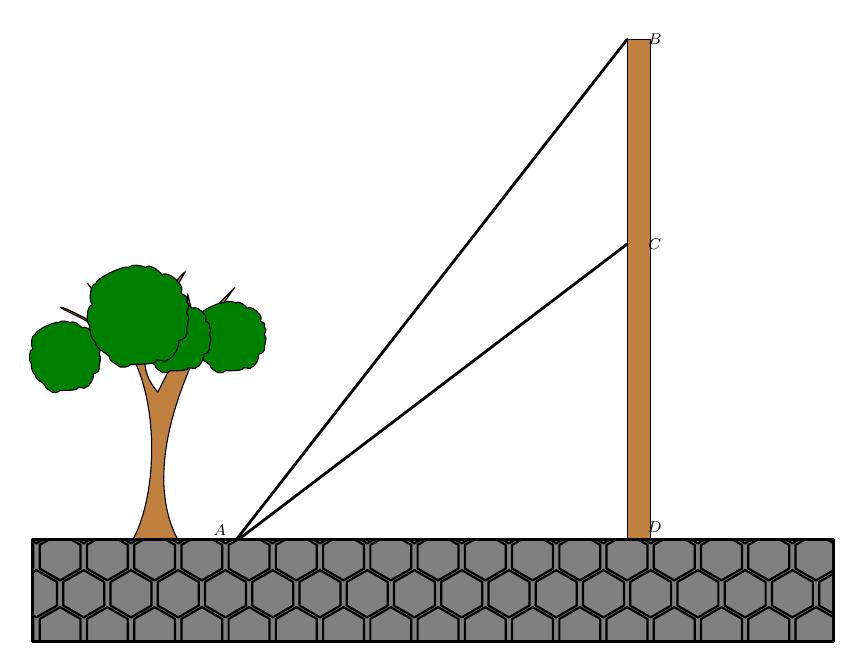
\begin{tikzpicture}[line join = round,line cap=round,>=stealth,font=\footnotesize,scale=1]
				 \draw[fill=brown]
					(0.00,0.00)..  controls +(60:0.7) and +(-60:0.7).. (0.00,2.40)
					.. controls +(130:0.45)  and +(-40:0.1).. (-0.90,3.00)
					.. controls +(0:0.1) and +(160:0.3)..  (-0.05,2.60)
					 -- (-0.55,3.30) -- (0.12,2.45)
					.. controls +(90:0.3)  and +(-115:0.4).. (0.12,3.45)
					 .. controls +(-90:0.3) and +(105:0.3).. (0.19,2.75)
					.. controls +(60:0.3) and +(-150:0.1).. (0.69,3.45) 
					.. controls +(-120:1)  and +(130:0.5).. (0.34,1.92)
					-- (0.72,2.67) --(0.72,3.17)  -- (0.82,2.75) -- (1.32,3.25)
					.. controls +(-140:0.1)  and +(120:1.4).. (0.62,0.00)--cycle;
				\tikzset{khomcay/.pic={ 
				 \draw[fill=green!50!black]
					(0.00,3.25).. controls +(-140:0.1) and  +(0:0.1).. (-0.20,3.20)
					.. controls  +(140:0.1) and +(-90:0.1).. (-0.40,3.40)
					.. controls +(140:0.1) and  +(-90:0.1).. (-0.65,3.65)
					..  controls +(140:0.1) and +(-90:0.1).. (-0.75,3.95)
					..  controls +(140:0.1) and +(180:0.1).. (-0.70,4.33)
					..  controls +(140:0.1) and +(180:0.1).. (-0.64,4.71)
					.. controls  +(90:0.1) and +(160:0.1).. (-0.04,5.01)
					..  controls +(40:0.1) and +(160:0.1).. (0.26,5.01)
					..  controls +(40:0.1) and +(120:0.1).. (0.56,4.87)
					.. controls  +(40:0.1) and +(120:0.1).. (0.86,4.73)
					.. controls +(-40:0.1)  and +(80:0.1).. (0.91,4.53)
					.. controls +(-20:0.1) and +(80:0.1).. (1.01,4.38) 
					 .. controls +(-40:0.1) and +(80:0.1).. (1.01,4.18)
					 .. controls +(-40:0.1) and +(80:0.1).. (1.01,3.88)
					.. controls +(-70:0.1) and  +(0:0.1).. (0.86,3.68)
					.. controls +(-70:0.1)  and +(0:0.1).. (0.66,3.33)
					.. controls +(-70:0.05) and  +(0:0.05).. (0.46,3.33)
					.. controls +(-70:0.1)  and +(0:0.1).. cycle;
					}} 
				 \path
					(-0.9,0.35) pic[scale=0.7]{khomcay} 
					(1.2,0.6) pic[scale=0.7]{khomcay} 
					(0.5,0.6) pic[scale=0.7]{khomcay} 
					(0,0)  pic{khomcay};
				\draw[fill=brown]  (6.3,0.05) rectangle (6.6,6.4);
				 \draw[line width=1pt]
					 (1.3,0) node[above left]{$A$} -- (6.3,6.4) node[right=0.25cm]{$B$}
					(1.3,0)  -- (6.3,3.8) node[right=0.25cm]{$C$};
				 \draw (6.3,0.2) node[right=0.25cm]{$D$};
				\begin{scope}
					\draw[line width=1pt,fill=gray] (-1.25,0.05) rectangle  (8.92,-1.25);
					\clip  (-1.25,0.05) rectangle (8.92,-1.25);
					\foreach  \y in {-3,-2,...,5}{
						\foreach \x in {-3,-2,...,15}{ 
						 \pgfmathsetmacro\shift{mod (\y,2)*0.3}
						\draw[thick] (\x*0.6 + \shift,\y * 0.47) 
						++(30:0.3) \foreach \a in {90,150,...,330}{ 
						 -- ++(\a:0.3)
						 } -- cycle;
					 }
					 }
				\end{scope}
			\end{tikzpicture}
	\end{center}
	\shortans{14,5} 
	 \loigiai{
		 Ta có
		 $
		 \tan\alpha=\tan (\widehat{BAD}-\widehat{CAD})
		 =\dfrac{\tan\widehat{BAD}-\tan\widehat{CAD}}{1+\tan\widehat{BAD}\tan\widehat{CAD}}=\dfrac{\dfrac{15}{12}-\dfrac{9}{12}}{1+\dfrac{15}{12}\cdot\dfrac{9}{12}}=\dfrac{8}{31}.
		 $\\
		Vì  vậy $\alpha\approx 14,47^\circ$.
	} 
\end{ex}

% từ: cau-hoi/lop11/1D1_Ham_so_luong_giac_va_phuong_trinh_luong/1D1-3-7_Toan_thuc_te_ap_dung_cong_thuc_luong_giac.tex
\begin{ex}%[1D1V3-7]%[ma:d02742db]
	\immini{ Trên nóc một tòa nhà có một cột ăngten cao $5$ m. Từ vị trí quan sát $A$ cao $7$ m so với mặt đất, có thể nhìn thấy đỉnh $B$ và chân $C$ của cột ăngten dưới góc  $\alpha$ và $\beta$ so với phương nằm ngang. Biết chiều cao của toà nhà là $18{,}9$ m, hai toà nhà cách nhau $10$ m. Tính góc $\alpha$ (làm tròn kết quả đến hàng đơn vị theo đơn vị độ).}{
	\begin{tikzpicture}[scale=.4,font=\footnotesize,line join=round,>=stealth,thick]
			\coordinate  (O) at (0,0);
			\def\nhathap{2} 
			 \def\nhacao{5}
			\def\kc{10} 
			\def\dai{1} 
			\def\cao{2} 
			\coordinate (H) at  (\kc,0);
			\newcommand{\xaynha}[2]{ 
			 \draw[very thick] (#1,#2) rectangle (#1+\dai,#2+\cao);
			 \draw[very thick,fill=black] (#1,#2) rectangle (#1+\dai,#2+0.25*\cao);
			\draw[very thick] (#1+0.2*\dai,#2+0.25*\cao) rectangle (#1+0.8*\dai,#2+0.9*\cao); 
			} 
			 \foreach \j in {1,...,\nhathap}{
				 \foreach \i in {0,...,4}{
				\xaynha{\i*1.1}{\j*\cao} 
			} 
			} 
			\draw[line width=0.2cm] (-0.1,\cao*\nhathap+\cao)--(5*\dai*1.1,\cao*\nhathap+\cao); 
			 \foreach \j in {1,...,\nhacao}{
				\foreach \i in {0,...,4}{ 
				 \xaynha{\i*1.1+\kc}{\j*\cao}
			} 
			} 
			\draw[line  width=0.2cm] (-0.1+\kc,\cao*\nhacao+\cao)--(5*\dai*1.1+\kc,\cao*\nhacao+\cao);
			 \coordinate (A) at (5*\dai*1.1,\cao*\nhathap+\cao+0.1);
			\draw (A) node[above  left]{$A$};
			\coordinate (C) at (\kc,\cao*\nhacao+\cao); 
			\draw (C)  node[above right]{$C$};
			\coordinate (B) at  ($(C)+(0,2)$);
			\draw  (B) node[above]{$B$};
			\coordinate (H) at (\kc,\cao); 
			\draw (H)  node[below]{$H$};
			\coordinate (D)  at (\kc,\cao*\nhathap+\cao+0.1);
			 \draw (D) node[above left]{$D$};
			\draw[very thick] (-0.5,\cao)--(\kc+5*\dai*1.2,\cao); 
			\draw [dashed](A)--(D); \draw (B)--(A)--(C); \draw[line width=0.07cm]  (C)--(B);
			 \draw ($(B)+(135:0.5cm)$)--($(B)+(-45:0.5cm)$);
			 \pic["$40^\circ$",draw,angle radius=5mm,angle eccentricity=1.6]{angle=D--A--C};
			\pic["$50^\circ$",draw,double,angle radius=12mm,angle  eccentricity=1.3]{angle=D--A--B};
			 \path ($(C)!0.55!(B)$) node [right]{$5\mathrm{\,m}$};
			\path ($(D)!0.5!(H)$) node  [left]{$7\mathrm{\,m}$};
		\end{tikzpicture}
	}\shortans{59} 
	\loigiai{ 
		Ta có: $AD=10$ mét  và $CD=18{,}9-7=11{,}9$ mét; $BD=BC+CD=11{,}9+5=16{,}9$ mét.\\
		Suy ra $\tan  \alpha=\dfrac{BD}{AD}=\dfrac{16{,}9}{10}$ $\Rightarrow \alpha\approx59^{\circ}$.
	 }
\end{ex}

% từ: cau-hoi/lop11/1D1_Ham_so_luong_giac_va_phuong_trinh_luong/1D1-4-6_Tim_tap_gia_tri_va_min_max.tex
\begin{bt}%[1D1H4-6]%[ma:7fa12eee]
% nguon: Archive/SP_KhoLatex/ID6_old/1K1-ot.tex #3775
%[Dự án 2 - TLDH - TeamTeXHoa - Quang Ngô]
    Tìm tập giá trị của các hàm sau:
    \begin{listEX}[2]
        \item $y=2 \cos\left(2x-\dfrac{\pi}{3}\right)-1$. 
        \item $y= \sin x+ \cos x$.
    \end{listEX}
    \loigiai{
        \begin{enumerate}
            \item Ta có\\
            \begin{eqnarray*}
                && -1\le \cos\left(2x-\dfrac{\pi}{3}\right)\le 1  ,\;\forall x\in \mathbb{R}. \\ 
                & \Leftrightarrow&-2\le 2 \cos\left(2x-\dfrac{\pi}{3}\right)\le 2  ,\;\forall x\in \mathbb{R}. \\ 
                & \Leftrightarrow&-2-1\le 2 \cos\left(2x-\dfrac{\pi}{3}\right)-1\le 2-1  ,\;\forall  x\in \mathbb{R}\\ 
                & \Leftrightarrow&-3\le 2 \cos\left(2x-\dfrac{\pi}{3}\right)-1\le 1  ,\;\forall  x\in \mathbb{R} \\ 
                & \Leftrightarrow&-3\le y\le 1  ,\;\forall  x\in \mathbb{R}.
            \end{eqnarray*}
            Vậy tập giá trị của hàm số $y=2\cos\left(2x-\dfrac{\pi}{3}\right)-1$ là $\left[ -3;1\right]$.
            \item Ta có
            \begin{eqnarray*}
                 \sin x+\cos x &=&\sqrt{2}\left(\dfrac{1}{\sqrt{2}} \sin x+\dfrac{1}{\sqrt{2}} \cos x\right) \\ 
                 &=&\sqrt{2}\left(\cos\dfrac{\pi}{4} \sin x+ \sin\dfrac{\pi}{4} \cos x\right) \\ 
                 &=&\sqrt{2}\left(\sin x \cos\dfrac{\pi}{4}+ \cos x \sin\dfrac{\pi}{4}\right) \\ 
                 &=&\sqrt{2} \sin\left(x+\dfrac{\pi}{4}\right).
            \end{eqnarray*}
            Khi đó ta có hàm số $ y=\sqrt{2} \sin\left(x+\dfrac{\pi}{4}\right)$.\\
            Lại có: $-1\le \sin\left(x+\dfrac{\pi}{4}\right)\le 1$ với mọi $ x\in \mathbb{R}$.\\
            $\Leftrightarrow-\sqrt{2}\le \sqrt{2} \sin\left(x+\dfrac{\pi}{4}\right)\le \sqrt{2}$ với mọi $x\in \mathbb{R}$.\\
            $\Leftrightarrow-\sqrt{2}\le y\le \sqrt{2}$ với mọi $x\in \mathbb{R}$.\\
            Vậy tập giá trị của hàm số $ y= \sin x+ \cos x$ là $\left[-\sqrt{2};\sqrt{2}\right]$.
        \end{enumerate}
    }
\end{bt}

% từ: cau-hoi/lop11/1D1_Ham_so_luong_giac_va_phuong_trinh_luong/1D1-5-3_Phuong_trinh_co_ban_dung_Radian.tex
\begin{ex}%[1D1H5-3]%[ma:2a012f6c]
 Kết quả khảo sát cân nặng của $25$ quả cam ở mỗi lô hàng ${A, B}$ được cho  ở bảng sau
 \begin{center}
  \begin{tabular}{|c|c|c|c|c|c|}
   \hline 
   Cân nặng (gam)  & $[150; 155)$ & $[155; 160)$ & $[160; 165)$ & $[165; 170)$ & $[170; 175)$ \\ \hline
   Số quả cam ở  lô hàng $A$ & 2 & 6 & 12 & 4 & 1 \\ \hline
   Số quả cam ở lô hàng $B$ & 1 & 3 &  7 & 10 & 4 \\ \hline
  \end{tabular}
 \end{center}
  \choiceTF
  {\True Giá trị  đại diện nhóm $[150; 155)$ bằng $152{,}5$}
   {Cân nặng trung bình của mỗi quả cam ở lô $A$ là $163{,}7$ (gam)}
  {Cân nặng trung bình của mỗi quả cam  ở lô $B$ là $162{,}1$ (gam)}
  {\True Theo số trung bình thì cam ở lô hàng ${B}$ nặng hơn  cam ở lô hàng $A$}
  \loigiai{
  \begin{itemchoice}
   \itemch \textbf{Đúng}. Bảng thống  kê số lượng cam theo giá trị đại diện
   \begin{center}
    \begin{tabular}{|c|c|c|c|c|c|}
      \hline
     Cân nặng (gam)  & $152{,}5$ & $157{,}5$ & $162{,}5$ & $167{,}5$ & $172{,}5$ \\ \hline
     Số quả cam ở lô hàng $A$  & 2 & 6 & 12 & 4 & 1 \\ \hline
     Số quả cam ở lô hàng $B$ & 1 & 3 & 7  & 10 & 4 \\ \hline
    \end{tabular}
   \end{center}
   \itemch  \textbf{Sai}. Cân nặng trung bình của mỗi quả cam ở lô $A$ là
   $${\bar{x}_A=\dfrac{152{,}5 \cdot 2+157{,}5  \cdot 6+162{,}5 \cdot 12+167{,}5 \cdot 4+172{,}5 \cdot 1}{25}=161{,}7 \text { (gam).}
   }$$ 
   \itemch \textbf{Sai}. Cân nặng trung  bình của mỗi quả cam ở lô $B$ là
   $${\bar{x}_B=\dfrac{152,5 \cdot 1+157,5 \cdot 3+162,5 \cdot 7+167,5 \cdot 10+172,5 \cdot 4}{25}=165,1 \text {  (gam).}
   }$$ 
   \itemch \textbf{Đúng}. Ta thấy ${\bar{x}_A<\bar{x}_B}$. Vậy nếu so sánh theo số trung bình thì cam ở lô hàng $B$ nặng hơn cam ở lô hàng $A$. 
  \end{itemchoice}
  }
\end{ex}

% từ: cau-hoi/lop11/1D1_Ham_so_luong_giac_va_phuong_trinh_luong/1D1-5-3_Phuong_trinh_co_ban_dung_Radian.tex
\begin{ex}%[1D1H5-3]%[ma:1650d46f]
 Số câu  trả lời đúng một bài thi trắc nghiệm môn Sinh học gồm 50 câu của lớp 11A ở một trường THPT như sau
 \begin{center}
  \begin{tabular}{|c|c|c|c|c|c|}
    \hline
   Thâm niên (Số năm) & $[14;21)$ &  $[21; 28)$ & $[28;35)$ & $[35; 42)$ & $[42;49)$ \\ \hline
   Số giáo viên & 4  & 8 & 25 & 6 & 7 \\ \hline
  \end{tabular}
 \end{center}
 \choiceTF 
  {\True  Giá trị đại diện của nhóm $[14; 21)$ là $17{,}5$}
  {\True Giá trị đại diện của  nhóm $[21; 28)$ là $24{,}5$}
  {\True Giá trị đại diện  của nhóm $[42; 49)$ là $45{,}5$}
  {Số câu đúng  trung bình là $32{,}26$}
  \loigiai{
  \begin{itemchoice}
   \itemch \textbf{Đúng}. Giá trị đại diện của nhóm $[14; 21)$ là  $17{,}5$.
   \itemch \textbf{Đúng}.Giá trị đại diện của nhóm $[21; 28)$  là $24{,}5$.
   \itemch \textbf{Đúng}. Giá trị đại diện của nhóm $[42; 49)$ là $45{,}5$. 
   \itemch \textbf{Sai}. 
   \begin{center}
    \begin{tabular}{|c|c|c|c|c|c|}
      \hline
     Thâm niên  (Số năm) & $[14;21)$ & $[21; 28)$ & $[28;35)$ & $[35; 42)$ & $[42;49)$ \\ \hline
     Giá trị đại diện & $17{,}5$ &  $24{,}5$ & $31{,}5$ & $38{,}5$ & $45{,}5$ \\ \hline
     Số giáo viên & 4 & 8 & 25 &  6 & 7 \\ \hline
    \end{tabular}
   \end{center}
   Số  câu đúng trung bình
    $$\bar{x}=\dfrac{4\cdot17{,}5+8\cdot24{,}5+25\cdot31{,}5+6\cdot38{,}5+7\cdot45{,}5}{50}=32{,}06.$$
  \end{itemchoice}
  }
\end{ex}

% từ: cau-hoi/lop11/1D1_Ham_so_luong_giac_va_phuong_trinh_luong/1D1-5-3_Phuong_trinh_co_ban_dung_Radian.tex
\begin{bt}%[1D1N5-3]%[ma:0f6652df]
% nguon: Archive/2024/SP-K10-K11-LyVanHoang_TVN-023/11. C1-LuongGiac-lvhoang_TVN-023/dataC1K11/Chuong1-Bai4-Dang3-PhuongTrinhCBDungRadian.tex #1627
[Mức N, CTST]%[BG Toán 11 CT2025, Quan Ón]
	Giải các phương trình
	\begin{listEX}[5]
		\item $\sin x=\dfrac{1}{2}$.
		\item $\cos x=-\dfrac{1}{2}$.
		\item $\tan x=\sqrt{3}$.
		\item $\cot x=-\dfrac{\sqrt{3}}{3}$.
		\item $\sin x = -\dfrac{5}{2}$.
	\end{listEX}
	\loigiai{
		\begin{enumerate}
			\item $\sin x = \dfrac{1}{2} \Leftrightarrow \sin x = \sin\dfrac{\pi}{6} \Leftrightarrow \hoac{&x = \dfrac{\pi}{6} + k2\pi\\&x = \pi - \dfrac{\pi}{6} + k2\pi} \Leftrightarrow \hoac{&x = \dfrac{\pi}{6} + k2\pi\\&x = \dfrac{5\pi}{6} + k2\pi}$ $(k\in\mathbb{Z})$.
			\item $\cos x = -\dfrac{1}{2} \Leftrightarrow \cos x = \cos\dfrac{2\pi}{3} \Leftrightarrow \hoac{&x = \dfrac{2\pi}{3} + k2\pi\\&x = -\dfrac{2\pi}{3} + k2\pi}$ $(k\in\mathbb{Z})$.
			\item $\tan x = \sqrt{3} \Leftrightarrow \tan x = \tan\dfrac{\pi}{3} \Leftrightarrow x = \dfrac{\pi}{3} + k\pi$, $(k\in\mathbb{Z})$.
			\item $\cot x = -\dfrac{\sqrt{3}}{3} \Leftrightarrow \cot x = \cot\left(-\dfrac{\pi}{3}\right) \Leftrightarrow x = -\dfrac{\pi}{3} + k\pi$, $(k\in\mathbb{Z})$.
			\item Vì $\left|-\dfrac{5}{2} \right| = \dfrac{5}{2} > 1$, do đó phương trình $\sin x = -\dfrac{5}{2}$ vô nghiệm.
		\end{enumerate}
	}
\end{bt}

% từ: cau-hoi/lop11/1D1_Ham_so_luong_giac_va_phuong_trinh_luong/1D1-5-5_Phuong_trinh_dua_ve_dang_co_ban.tex
\begin{ex}%[1D1V5-5]%[ma:73731a94]
	Giải  các phương trình sau
	\begin{listEX}[3]
		 \item $\sin x=-\dfrac{\sqrt{3}}{2}$;
		\item  $\sin x=\dfrac{1}{4}$;
		\item $\sin \left(x-60^\circ\right)=\dfrac{1}{2}$; 
		\item  $\sin x=1$;
		\item in  $3x=-\dfrac{4}{3}$;
		\item $\sin  (2019x+2020)=2$;
		\item  $\sin 3x=\dfrac{1}{2}$;
		\item $\sin  \left(\dfrac{x}{2}+\dfrac{\pi}{3}\right)=-\dfrac{\sqrt{3}}{2}$;
		 \item $2\sin (3x+1)=1$;
		\item  $\sin \left[\sin \left(x+\dfrac{\pi}{3}\right)\right]=0$;
		\item $\sin  \left(2x+\dfrac{\pi}{2}\right)=\sin \left(x-\dfrac{\pi}{3}\right)$;
		\item  $\sin^23x=\dfrac{3}{4}$;
		\item $\sin 2x-\cos x=0$; 
		\item $\sin  3x+\sin x=0$;
		\item  $\sin x+\cos \left(2x+\dfrac{\pi}{3}\right)=0$.
	\end{listEX}
	\loigiai{ 
		\begin{enumerate}[a)]
			\item  $\sin x=-\dfrac{\sqrt{3}}{2}\Leftrightarrow\sin x=\sin \left(-\dfrac{\pi}{3}\right)\Leftrightarrow\hoac{&x=-\dfrac{\pi}{3}+k 2\pi
			\\&x=\dfrac{4\pi}{3}+k  2\pi}~(k \in\mathbb{Z})$.
			\item $\sin x=\dfrac{1}{4}\Leftrightarrow\hoac{&x=\arcsin  \left(\dfrac{1}{4}\right)+k 2\pi\\&
			x=\pi-\arcsin \left(\dfrac{1}{4}\right)+k  2\pi}~(k \in\mathbb{Z})$.
			\item $\begin{aligned}
			\sin  \left(x-60^\circ\right)=\dfrac{1}{2}&\Leftrightarrow\sin \left(x-60^\circ\right)=\sin 30^\circ\\&\Leftrightarrow\hoac{&{x-60^\circ=30^\circ+k 360^\circ}\\&
			{x-60^\circ=150^\circ+k 360^\circ}}~(k \in\mathbb Z) \\& \Leftrightarrow\hoac{&x=90^\circ+k 360^\circ\\& 
			x=210^\circ+k 360^\circ}~(k \in\mathbb{Z}). 
		\end{aligned}
		 $
		\item $\sin x=1\Leftrightarrow x=\dfrac{\pi}{2}+k 2\pi~(k \in\mathbb{Z})$. 
		\item Ta có  $\sin 3x\in[-1; 1]\Rightarrow\sin 3x=-\dfrac{4}{3}$ vô nghiệm.
		\item Ta có $\sin (2019x+2020)  \in[-1; 1]\Rightarrow\sin (2019x+2020)=2$ vô nghiệm.
		\item $\begin{aligned}
		\sin 3x=\dfrac{1}{2}&\Leftrightarrow\sin 3x=\sin  \dfrac{\pi}{6}\\& \Leftrightarrow\hoac{&{3x=\dfrac {\pi} 6+k 2\pi}\\&
		{3x=\dfrac  {5\pi} 6+k 2\pi}}\\&\Leftrightarrow\hoac{&x=\dfrac{\pi}{18}+\dfrac{k 2\pi}{3}\\&
		x=\dfrac{5\pi}{18}+\dfrac{k 2\pi}{3}}~(k  \in\mathbb{Z}).
	\end{aligned}$
	\item $\begin{aligned}
	 \sin \left(\dfrac{x}{2}+\dfrac{\pi}{3}\right)=-\dfrac{\sqrt{3}}{2}&\Leftrightarrow\sin \left(\dfrac{x}{2}+\dfrac{\pi}{3}\right)=\sin \left(-\dfrac{\pi}{3}\right)\Leftrightarrow\hoac{&\dfrac{x}{2}+\dfrac{\pi}{3}=-\dfrac{\pi}{3}+k 2\pi
	 \\&\dfrac{x}{2}+\dfrac{\pi}{3}=\dfrac{4\pi}{3}+k 2\pi}~(k \in\mathbb{Z})
	\\&\Leftrightarrow\hoac{&{\dfrac x 2=-\dfrac {2\pi}  3+k 2\pi}\\&
	{\dfrac x 2=\pi+k 2\pi}}~(k \in\mathbb Z) \Leftrightarrow\hoac{&x=-\dfrac{4\pi}{3}+k 4\pi\\& 
	x=2\pi+k 4\pi}~(k \in\mathbb{Z}). 
	\end{aligned}$
	\item $\begin{aligned}
	2\sin  (3x+1)=1&\Leftrightarrow\sin (3x+1)=\dfrac{1}{2}\Leftrightarrow\sin (3x+1)=\sin \dfrac{\pi}{6}\Leftrightarrow\hoac{&3x+1=\dfrac{\pi}{6}+k 2\pi\\&3x+1=\dfrac{5\pi}{6}+k2\pi}~(k \in\mathbb{Z})
	\\& 
	\Leftrightarrow\hoac{&{3x=\dfrac {\pi} 6-1+k  2\pi}\\&
	{3x=\dfrac  {5\pi} 6-1+k 2\pi}}~(k \in\mathbb Z) \Leftrightarrow\hoac{&x=\dfrac{\pi}{18}-\dfrac{1}{3}+\dfrac{k 2\pi}{3}\\&
	x=\dfrac{5\pi}{18}-\dfrac{1}{3}+\dfrac{k 2\pi}{3}}~(k \in\mathbb{Z}). 
	\end{aligned}$
	\item $\sin \left[\sin  \left(x+\dfrac{\pi}{3}\right)\right]=0\Leftrightarrow \sin \left(x+\frac{\pi}{3}\right)=k \pi~(k \in \mathbb{Z})$. \\
	Vì $\sin \left(x+\frac{\pi}{3}\right)\in[-1; 1]$ và $k \in \mathbb{Z}$ nên ta có $k=0$. \\ 
	Suy ra 
	 $
	\sin \left(x+\frac{\pi}{3}\right)=0\Leftrightarrow x+\frac{\pi}{3}=k \pi~(k \in \mathbb{Z}) \Leftrightarrow x=-\frac{\pi}{3}+k \pi~(k \in \mathbb{Z}). 
	$ 
	\item Ta có $\begin{aligned}
	&\sin \left(2x+\dfrac{\pi}{2}\right)=\sin  \left(x-\dfrac{\pi}{3}\right)
	\\&\Leftrightarrow\hoac{&{2x+\dfrac {\pi}  2=x-\dfrac {\pi} 3+k 2\pi}\\&
	{2x+\dfrac {\pi} 2=\pi-(x-\dfrac {\pi}  3)+k 2\pi}}~(k \in\mathbb Z)
	 \Leftrightarrow\hoac{&x=-\dfrac{5\pi}{6}+k 2\pi\\&x=\dfrac{5\pi}{18}+\dfrac{k 2\pi}{3}}~(k \in\mathbb{Z}).
	\end{aligned}$
	\item $\begin{aligned}
	 \sin^23x=\dfrac{3}{4} &\Leftrightarrow\hoac{&\sin 3x=\dfrac{\sqrt{3}}{2}
	 \\&\sin 3x=-\dfrac{\sqrt{3}}{2}}\\
	&\Leftrightarrow\hoac{&3x=\dfrac{\pi}3+k 2\pi\\& 
	3x=\dfrac{2\pi}3+k  2\pi\\&
	3x=-\dfrac{\pi}3+k 2\pi\\& 
	3x=\dfrac{4\pi}3+k 2\pi 
	 }~(k \in\mathbb Z) \Leftrightarrow\hoac{&x=\dfrac{\pi}{9}+k \dfrac{2\pi}{3}\\&
	 x=\dfrac{2\pi}{9}+k \dfrac{2\pi}{3}\\&
	x=-\dfrac{\pi}{9}+k \dfrac{2\pi}{3}\\& 
	 x=\dfrac{4\pi}{9}+k \dfrac{2\pi}{3}
	 }~(k \in\mathbb{Z}).
	\end{aligned}$
	\item $\begin{aligned}
	 \sin 2x-\cos x=0&\Leftrightarrow\sin 2x=\cos x \Leftrightarrow\sin 2x=\sin \left(\dfrac{\pi}{2}-x\right)
	\\&\Leftrightarrow\hoac{&{2x=\dfrac {\pi} 2-x+k 2\pi}\\& 
	{2x=\dfrac {\pi} 2+x+k  2\pi}
	 }~(k \in\mathbb Z) \Leftrightarrow\hoac{&x=\dfrac{\pi}{6}+k \dfrac{2\pi}{3}\\&
	x=\dfrac{\pi}{2}+k  2\pi
	}~(k  \in\mathbb{Z}).
	\end{aligned}$;
	\item $\begin{aligned}
	\sin 3x+\sin x=0&\Leftrightarrow\sin 3x=-\sin x \Leftrightarrow\sin 3x=\sin  (-x) \\&
	\Leftrightarrow\hoac{&{3x=-x+k  2\pi}\\&
	{3x=\pi+x+k 2\pi} 
	}~(k \in\mathbb Z) \Leftrightarrow\hoac{&x=k  \dfrac{\pi}{2}\\&
	 x=\dfrac{\pi}{2}+k \pi
	 }~(k \in\mathbb{Z}) \Leftrightarrow x=k \dfrac{\pi}{2}~(k \in\mathbb{Z}).
	\end{aligned}$
	\item $\begin{aligned}
	\sin x+\cos \left(2x+\dfrac{\pi}{3}\right)=0&\Leftrightarrow\sin x=-\cos  \left(2x+\dfrac{\pi}{3}\right)\Leftrightarrow\sin x=\sin \left(2x-\dfrac{\pi}{6}\right)
	 \\&\Leftrightarrow\hoac{&{x=2x-\dfrac {\pi} 6+k 2\pi}\\&
	{x=\dfrac {7\pi} 6-2x+k  2\pi}
	}~(k \in\mathbb Z) \Leftrightarrow\hoac{&x=\dfrac{\pi}{6}-k 2\pi\\& 
	x=\dfrac{7\pi}{18}+k  \dfrac{2\pi}{3}
	}~(k \in\mathbb{Z}). 
	\end{aligned}$
	\end{enumerate}
 }
\end{ex}

% từ: cau-hoi/lop11/1D1_Ham_so_luong_giac_va_phuong_trinh_luong/1D1-5-5_Phuong_trinh_dua_ve_dang_co_ban.tex
\begin{bt}%[1D1H5-5]%[ma:04c1052d]
% nguon: Archive/2024/SP-K10-K11-LyVanHoang_TVN-023/11. C1-LuongGiac-lvhoang_TVN-023/dataC1K11/Chuong1-Bai4-Dang5-Phuongtrinhduavecoban.tex #2025
%[Bài giảng 11, Trần Tony]
	Giải các phương trình sau
	\begin{listEX}[2]
		\item $\sqrt{3}\sin x+\cos x=2$.
		\item $3\sin x + \cos x = 2$.
		\item $\sqrt{3}\cos 2x+\sin 2x-\sqrt{3}=0$.
		\item $\sin x+3\cos x=5$.
	\end{listEX}
	\loigiai{
		\begin{enumerate}[a)]
			\item Phương trình tương đương $\dfrac{\sqrt{3}}{2}\sin x+\dfrac{1}{2}\cos x=1\Leftrightarrow \sin \dfrac{\pi}{3}\sin x +\cos \dfrac{\pi}{3}\cos x=1$\\
			$\Leftrightarrow \cos \left( x-\dfrac{\pi}{3}\right) =1\Leftrightarrow x=\dfrac{\pi}{3}+k2\pi$ $(k\in \mathbb{Z})$.
			
			\item  $3\sin x + \cos x = 2 \Leftrightarrow \dfrac{3}{\sqrt {10} }\sin x + \dfrac{1}{\sqrt {10}}\cos x = \dfrac{2}{\sqrt {10} }$.\hfill$(1)$\\
			Đặt $\dfrac{1}{\sqrt {10}} = \cos \alpha $ và
			$\dfrac{3}{\sqrt {10}} = \sin \alpha $,  thay vào (1), ta được
			{\allowdisplaybreaks
				\begin{align*}
					&\cos x\cos \alpha  + \sin x\sin \alpha  = \frac{2}{\sqrt {10} } \Leftrightarrow \cos (x - \alpha ) = \frac{2}{\sqrt {10}}=\cos\beta\\
					\Leftrightarrow& 
					\hoac{&x - \alpha  = \beta + k2\pi \\&
						x - \alpha  =  - \beta + k2\pi}
					\Leftrightarrow\hoac{&x = \alpha  + \beta + k2\pi \\&x = \alpha  - \beta + k2\pi.}
			\end{align*}}
			\item Ta có
			\begin{align*}
				\sqrt{3}\cos 2x+\sin 2x-\sqrt{3}=0&\Leftrightarrow \sqrt{3}\cos 2x+\sin 2x=\sqrt{3}.\\
				&\Leftrightarrow \dfrac{\sqrt{3}}{2}\cos 2x+\dfrac{1}{2}\sin 2x=\dfrac{\sqrt{3}}{2}\\
				&\Leftrightarrow \sin\left(2x+\dfrac{\pi}{3}\right)=\dfrac{\sqrt{3}}{2}\\
				&\Leftrightarrow \hoac{&2x+\dfrac{\pi}{3}=\dfrac{\pi}{3}+k2\pi\\ &2x+\dfrac{\pi}{3}=\dfrac{2\pi}{3}+k2\pi.}\Leftrightarrow \hoac{&x=k\pi\\ &x=\dfrac{\pi}{6}+k\pi}, (k\in\mathbb{Z}).
			\end{align*}
			\item Vì $1^2+3^2<5^2$ nên phương trình vô nghiệm.
		\end{enumerate}
	}
\end{bt}

% từ: cau-hoi/lop11/1D1_Ham_so_luong_giac_va_phuong_trinh_luong/1D1-5-5_Phuong_trinh_dua_ve_dang_co_ban.tex
\begin{bt}%[1D1N5-5]%[ma:e519e1de]
% nguon: Archive/SP_KhoLatex/ID6_old/1D1Y3-5.tex #2967
%[Đề thi Học Kì 1, 2016 - 2017 trường THPT Nguyễn Thị Minh Khai, Hồ Chí Minh]%[Phạm Doãn Lê Bình, 11-HK1-18]
	Giải phương trình $\cos^2 x - \sin^2 x = \sin 3x + \cos 4x$.
\loigiai{
	Phương trình ban đầu tương đương với 
		\begin{align*}
		& \cos 2x = \sin 3x + \cos 4x \Leftrightarrow \sin 3x + \cos 4x - \cos 2x = 0 \\
		\Leftrightarrow & \sin 3x - 2\sin 3x \sin x = 0 \Leftrightarrow \sin 3x (1-2\sin x)=0\\
		\Leftrightarrow & \hoac{& \sin 3x = 0 \\ & \sin x = \dfrac{1}{2}} \Leftrightarrow \hoac{& x = \dfrac{k\pi}{3} \\ & x = \dfrac{\pi}{6}+k2\pi \\ & x = \dfrac{5\pi}{6}+k2\pi}, (k\in\mathbb{Z}).
		\end{align*}
Vậy tập nghiệm của hệ phương trình là $S=\{ \dfrac{k\pi}{3}; \dfrac{\pi}{6}+k2\pi; \dfrac{5\pi}{6}+k2\pi|k\in\mathbb{Z}\}$.
}
\end{bt}

% từ: cau-hoi/lop11/1D1_Ham_so_luong_giac_va_phuong_trinh_luong/1D1-5-6_Toan_thuc_te_ap_dung_phuong_trinh_luong_giac.tex
\begin{ex}%[1D1C5-6]%[ma:7c850c88]
	Một cây cầu có dạng cung $OA$ là một  phần của đồ thị hàm số $y=4{,}8 \sin \dfrac{x}{9}$ và được mô tả trong hệ trục tọa độ với đơn vị trục là mét như hình bên.
	\begin{center}
		\begin{tikzpicture}[line join=round,line cap=round,>=stealth,scale=.85,transform shape]
				\def\xmin{0}  \def\xmax{12} \def\ymin{-.5} \def\ymax{2}
				\draw[->](\xmin-.5,0)--(\xmax+1,0) node[below]{$x$}; 
				\draw[->](0,\ymin)--(0,\ymax+.5) node[left]{$y$}; 
				\draw (0,0) node[below right]{$O$}; 
				\draw  (\xmin,0) to [out=40,in= 140] (\xmax,0) node[below]{$A$};
			\end{tikzpicture}
	\end{center}
	Giả sử chiều rộng của con sông là độ  dài đoạn thẳng $OA$. Chiều rộng đó (làm tròn đến kết quả hàng phần mười) là
	\shortans{28,3} 
	\loigiai{ 
		 Phương trình hoành độ giao điểm
		$$4{,}8 \sin  \dfrac{x}{9}=0\Leftrightarrow\sin \dfrac{x}{9}=0\Leftrightarrow\dfrac{x}{9}=k\pi\Leftrightarrow x=9k\pi,\ (k\in \mathbb{Z}).$$
		Hoành độ điểm $A$ ứng  với $x=9\pi$.\\
		Vậy  $OA=9\pi\approx 28{,}3$m.
	} 
\end{ex}

% từ: cau-hoi/lop11/1D1_Ham_so_luong_giac_va_phuong_trinh_luong/1D1-5-6_Toan_thuc_te_ap_dung_phuong_trinh_luong_giac.tex
\begin{bt}%[1D1V5-6]%[ma:521f7339]
% nguon: Archive/2024/TOAN_11_XE/TOAN_11_XE/data4/11C1/KNTT-1.4.tex #1092
 
	\immini{Một cây cầu có dạng cung $AB$ của đồ thị hàm số $y=4{,}2\cdot\cos\dfrac{x}{8}$ và được mô tả trong hệ trục toạ độ với đơn vị trục là mét như ở hình bên. Một sà lan chở khối hàng hoá được xếp thành hình hộp chữ nhật với độ cao $3$ m so với mực nước sông sao cho sà lan có thể đi qua được gầm cầu. Chứng minh rằng chiều rộng của khối hàng hoá đó phải nhỏ hơn $12{,}5$ m.}{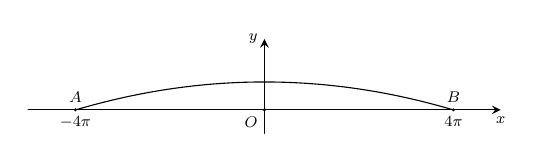
\begin{tikzpicture}[scale=0.6, font=\footnotesize, line join=round, line cap=round,>=stealth]
			\def\a{0} \def\b{-0.037} \def\c{0.59} % Hệ số
			\def\xmin{-5} \def\xmax{5}
			\def\ymin{-.5} \def\ymax{1.5}		
			\draw[->] (\xmin,0)--(\xmax,0) node [below]{$x$};
			\draw[->] (0,\ymin)--(0,\ymax) node [left]{$y$};
			\node at (0,0) [below left]{$O$};
			\fill (0,0)circle (1.0pt) (-4,0)node[above]{$A$} circle (1.0pt) (4,0)node[above]{$B$} circle (1.0pt) circle (1.0pt) (-4,0)node[below]{$-4\pi$} circle (1.0pt) (4,0)node[below]{$4\pi$} circle (1.0pt);
			\clip (-4,0) rectangle (4,1);
			\draw[smooth,samples=300] plot(\x,{\a*(\x)^4+\b*(\x)^2+\c});
	\end{tikzpicture}}
	\loigiai{
		Với mỗi điểm $ M $ nằm trên mặt cầu, khoảng cách từ điểm $ M $ đến mặt nước tương ứng với giá trị tung độ $ y $ của điểm $ M $,
		Xét phương trình $ 4{,}2\cdot \cos\dfrac{x}{8}=3\Leftrightarrow \cos \dfrac{x}{8}=\dfrac{5}{7}$.\\
		Do $ x\in [-4\pi;4\pi] $ nên $ \dfrac{x}{8}\in \left[-\dfrac{\pi}{2};\dfrac{\pi}{2} \right]  $.\\
		Khi đó, ta có $ \cos\dfrac{x}{8}=\dfrac{5}{7}\Leftrightarrow \dfrac{x}{8}\approx\pm 0{,}775 $, suy ra $ \left| \dfrac{x}{8}\right|<0{,}78\Leftrightarrow|x|<6{,}14$.\\
		Do sà lan có thể đi qua được gầm cầu nên chiều rộng của khối hàng hóa là $$ 2|x|<12{,}48<12{,}5. $$
	}
\end{bt}

% từ: cau-hoi/lop11/1D2_Day_so_Cap_so_cong_Cap_so_nhan/1D2-1-2_So_hang_tong_quat_bieu_dien_day_so.tex
\begin{ex}%[1D2V1-2]%[ma:1217bcf0]
	\immini{Cho hình vuông $A_1 B_1 C_1 D_1$  có cạnh bằng $4$. Với mọi số nguyên dương $n\ge 2$, gọi $A_n, B_n, C_n, D_n$ lần lượt là trung điểm của các cạnh $A_{n-1} B_{n-1}, B_{n-1} C_{n-1}, C_{n-1} D_{n-1}$, $D_{n-1} A_{n-1}$. Gọi $S_n$ là diện tích của tứ giác $A_n B_n C_n D_n$. Tính giá trị của biểu thức $2^{25}\cdot S_{12}$.}
	{\begin{tikzpicture}[>=stealth,line join=round,line cap=round,font=\footnotesize,scale=0.8]
		 \path
			(0,0) coordinate (D_1) 
			(5,0)  coordinate (C_1)
			($(D_1)!1!90:(C_1)$) coordinate  (A_1)
			 ($(A_1)+(C_1)-(D_1)$) coordinate (B_1)
			($(A_1)!1/2!(B_1)$) coordinate  (A_2)
			($(A_1)!1/2!(D_1)$) coordinate (D_2) 
			($(D_1)!1/2!(C_1)$) coordinate (C_2) 
			($(B_1)!1/2!(C_1)$) coordinate  (B_2)
			 ($(A_2)!1/2!(B_2)$) coordinate (A_3)
			($(A_2)!1/2!(D_2)$)  coordinate (D_3)
			($(D_2)!1/2!(C_2)$) coordinate  (C_3)
			($(B_2)!1/2!(C_2)$) coordinate (B_3) 
			($(A_3)!1/2!(B_3)$) coordinate  (A_4)
			($(A_3)!1/2!(D_3)$) coordinate  (D_4)
			($(D_3)!1/2!(C_3)$) coordinate  (C_4)
			($(B_3)!1/2!(C_3)$) coordinate  (B_4);
		 \draw
			 (A_1)--(B_1)--(C_1)--(D_1)--(A_1)
			(A_2)--(B_2)--(C_2)--(D_2)--(A_2) 
			 (A_3)--(B_3)--(C_3)--(D_3)--(A_3)
			 (A_4)--(B_4)--(C_4)--(D_4)--(A_4);
		\foreach \x/\y in {A_1/180,B_1/0,C_1/-10,D_1/190,A_2/90,B_2/0,C_2/-90,D_2/180,A_3/60,B_3/-60,C_3/230,D_3/160,A_4/0,B_4/-90,C_4/180,D_4/90} 
		\draw[fill=black] (\x) circle (1.1pt) + (\y:0.5cm) node  {$\x$};
	\end{tikzpicture}
	} 
	\shortans{1024} 
	\loigiai{ 
		Ta thấy mỗi  tứ giác $A_n B_n C_n D_n$ là một hình vuông có cạnh là $A_n B_n$.\\
		Ta có $A_1 B_1=4,A_2 B_2=\dfrac{1}{\sqrt{2}} A_1 B_1=2\sqrt{2}, A_3  B_3=\dfrac{1}{\sqrt{2}} A_2 B_2=\left(\dfrac{1}{\sqrt{2}} \right)^2 A_1 B_1=2,\ldots$\\
		Tổng quát $A_n B_n=\left(\dfrac{1}{\sqrt{2}} \right)^{n-1} A_1 B_1=\left(\dfrac{1}{\sqrt{2}}  \right)^{n-1} \cdot 4=\left(\dfrac{1}{\sqrt{2}} \right)^{n+3}$.\\
		Diện tích hình vuông $A_n B_n C_n D_n$  là $S_n=\left(A_n B_n \right)^2=\left(\dfrac{1}{2} \right)^{n+3}$, với mọi $n\in \mathbb{N}^*$.\\
		Áp dụng với $n=12$ có  $S_{12}=\left(\dfrac{1}{2} \right)^{15}$.\\
		Vậy $2^{12}\cdot  S_{12}=2^{25}\cdot \dfrac{1}{2^{15}}=1024$
	} 
\end{ex}

% từ: cau-hoi/lop11/1D2_Day_so_Cap_so_cong_Cap_so_nhan/1D2-2-2_Nhan_dien_cap_so_cong_cong_sai.tex
\begin{ex}%[1D2H2-2]%[ma:f48911b2]
	Cho dãy số $(u_n)$ xác định  bởi $u_n=(-1)^n-\cos \left(n \pi\right)$. Giá trị $u_{99}$ bằng
	 \choice
		{\True $0$} 
		{$-1$} 
		{$1$} 
		 {$99$}
	\loigiai{Giá trị $u_{99}$ bằng  $u_{99}=(-1)^{99}-\cos \left(99 \pi\right)=-1-(-1)=0$.
	 }
\end{ex}

% từ: cau-hoi/lop11/1D2_Day_so_Cap_so_cong_Cap_so_nhan/1D2-2-6_Tinh_tong_cua_cap_so_cong.tex
\begin{ex}%[1D2H2-6]%[ma:86dd0e92]
	Cho dãy số $(u_n)$ xác định bởi $\heva{&u_1=2\\& u_{n+1}=u_n+3, n \ge 1}$. Tìm  tổng $20$ số hạng đầu của dãy số $(u_n)$.
	\shortans{610} 
	\loigiai{ 
		Vì dãy số $(u_n)$ có $u_{n+1}=u_n+3, n \ge 1$ nên $(u_n)$ là cấp số cộng có $u_1=2$, công  sai $d=3$.\\
		Vậy tổng $20$ số hạng đầu của dãy số $(u_n)$  là $S_{20}=\dfrac{20}{2}[2u_1+19d]=10(2\cdot 2+19\cdot 3)=610$.
	} 
\end{ex}

% từ: cau-hoi/lop11/1D2_Day_so_Cap_so_cong_Cap_so_nhan/1D2-3-4_Tim_so_hang_cu_the_trong_cap_so_nhan.tex
\begin{ex}%[1D2V3-4]%[ma:b15c6fa6]
	Cho dãy số $\left(u_n\right)$ được xác định bởi $u_1=2$; $u_n=2u_{n-1}+3n-1$. Tìm số hạng thứ $2\,019$ của dãy  số.
	\choice 
		{\True  $u_{2\,019}=5\cdot 2^{2\,019}-6\,062$}
		{$u_{2\,019}=5\cdot 2^{2\,019}+6\,062$} 
		{$u_{2\,019}=5\cdot 2^{2\,020}-6\,062$} 
		{$u_{2\,019}=5\cdot  2^{2\,020}+6\,062$}
	\loigiai{ 
		Ta có $u_n=2u_{n-1}+3n-1 \Leftrightarrow {u_n}+3n+5=2\left[u_{n-1}+3\left(n-1\right)+5\right]$,  với $n\ge 2$; $n\in\mathbb{N}$.\\
		Đặt $v_n=u_n+3n+5$, ta  có $v_n=2v_{n-1}$ với $n\ge 2$; $n\in\mathbb{N}$.\\
		Như vậy, $\left(v_n\right)$ là cấp số nhân với công bội $q=2$ và  $v_1=10$, do đó $v_n=10\cdot 2^{n-1}=5\cdot 2^n$.\\
		Do đó  $u_n+3n+5=5\cdot 2^n$, hay $u_n=5\cdot 2^n-3n-5$ với $n\ge 2$; $n\in\mathbb{N}$.\\
		Nên $u_{2\,019}=5\cdot 2^{2\,019}-6\,062$. 
	} 
\end{ex}

% từ: cau-hoi/lop11/1D3_Gioi_han_Ham_so_lien_tuc/1D3-1-2_Phuong_phap_dat_thua_so_chung_lim_huu_han.tex
\begin{ex}%[1D3H1-2]%[ma:1f2a5708]
	Cho $\lim\limits_{n \to +\infty} \dfrac{an+1}{2n-4}=-5$ giá  trị của $a$ là
	\choice{\True  $-10$}
		 {$1$}
		{$0$} 
		 {$6$}
	\loigiai{ 
		Ta có $\lim\limits_{n \to +\infty} \dfrac{an+1}{2n-4}=-5\Leftrightarrow \lim\limits_{n \to +\infty} \dfrac{a+\dfrac{1}{n}}{2-\dfrac{4}{n}}=-5\Leftrightarrow \dfrac{a}{2}=-5\Leftrightarrow a=-10$. 
	 }
\end{ex}

% từ: cau-hoi/lop11/1D3_Gioi_han_Ham_so_lien_tuc/1D3-1-2_Phuong_phap_dat_thua_so_chung_lim_huu_han.tex
\begin{ex}%[1D3V1-2]%[ma:5455f73f]
	Cho cấp số cộng $\left(u_n \right)$ có số hạng đầu $u_1=2$ và công sai $d=3$. Tìm $\lim\dfrac{n}{u_n}$ 
	\choice 
		 {\True $L=\dfrac{1}{3}$}
		{$L=\dfrac{1}{2}$} 
		{$L=3$} 
		 {$L=2$}
	\loigiai{Ta có $u_n=u_1+\left(n-1\right)d=2+\left(n-1\right)3=3n-1$. Do  đó $\lim\dfrac{n}{u_n}=\lim\dfrac{n}{3n-1}=\lim\dfrac{1}{3-\dfrac{1}{n}}=\dfrac{1}{3}$.
	 }
\end{ex}

% từ: cau-hoi/lop11/1D3_Gioi_han_Ham_so_lien_tuc/1D3-1-3_Phuong_phap_luong_lien_hop_lim_huu_han.tex
\begin{ex}%[1D3H1-3]%[ma:24371bd3]
 Mỗi kết  quả giới hạn dưới đây đúng hay sai?
 \choiceTF 
   {$\lim\limits_{n \to +\infty} \left(\sqrt{n+3}-\sqrt{n+1}\right)=2$}
  {$\lim\limits_{n \to  +\infty} \left(n-\sqrt{n^2-1}\right)=-1$}
  {\True  $\lim\limits_{n \to +\infty} \dfrac{\sqrt{n+3}-\sqrt{n}}{n+2}=0$}
  {$\lim\limits_{n  \to +\infty}\left(\sqrt{n^2+2}-n\right)n=0$}
 \loigiai{ 
  \begin{itemchoice}
   \itemch $\lim\limits_{n \to  +\infty} \left(\sqrt{n+3}-\sqrt{n+1}\right)
   =\lim\limits_{n  \to +\infty} \dfrac{2}{\sqrt{n+3}+\sqrt{n+1}}
    =\lim\limits_{n \to +\infty} \dfrac{1}{\sqrt{n}\left(\sqrt{1+\dfrac{3}{n}}+\sqrt{1+\dfrac{1}{n}}\right)}=0$.
   \itemch $\lim\limits_{n \to +\infty} \left(n-\sqrt{n^2+1}\right)=\lim\limits_{n \to  +\infty} \dfrac{1}{n+\sqrt{n^2-1}}=\lim\limits_{n \to \infty} \dfrac{1}{n\left(1+\sqrt{1-\dfrac{1}{n^2}}\right)}=0$.
   \itemch $\lim\limits_{n \to +\infty}  \dfrac{\sqrt{n+3}-\sqrt{n}}{n+2}
   =\lim\limits_{n \to +\infty} \dfrac{3}{\left(\sqrt{n+3}+\sqrt{n}\right)(n+2)} 
   =\lim\limits_{n  \to +\infty} \dfrac{\dfrac{3}{n\sqrt{n}}}{\left(\sqrt{1+\dfrac{3}{n}}+\sqrt{n}\right)(1+\dfrac{2}{n})}=0$.
    \itemch $\lim\limits_{n \to +\infty}\left(\sqrt{n^2+2}-n\right)n
   =\lim\limits_{n  \to +\infty} \dfrac{2n}{\sqrt{n^2+2}+n}
   =\lim\limits_{n \to +\infty}  \dfrac{2}{\sqrt{1+\dfrac{2}{n^2}}+1}=1
    $.
  \end{itemchoice}
  }
\end{ex}

% từ: cau-hoi/lop11/1D3_Gioi_han_Ham_so_lien_tuc/1D3-1-5_Cap_so_nhan_lui_vo_han.tex
\begin{ex}%[1D3H1-5]%[ma:dd3507f9]
	Tính tổng $S$ của cấp số nhân lùi vô  hạn có số hạng đầu $u_{1}=1$ và công bội $q=-\dfrac{1}{2}$.
	\choice 
		{$S=2$} 
		 {$S=\dfrac{3}{2}$}
		 {$S=1$}
		 {\True $S=\dfrac{2}{3}$}
	 \loigiai{
		 Ta có $S=\dfrac{u_{1}}{1-q}=\dfrac{1}{1-\left(-\dfrac{1}{2}\right)}=\dfrac{2}{3}$.
	} 
\end{ex}

% từ: cau-hoi/lop11/1D3_Gioi_han_Ham_so_lien_tuc/1D3-1-5_Cap_so_nhan_lui_vo_han.tex
\begin{ex}%[1D3H1-5]%[ma:49582f6c]
	Cấp số nhân lùi vô hạn $\left(u_{n}\right)$ có $u_{1}=-2$; $q=\dfrac{1}{2}$. Khi đó tổng $S$ của cấp số  nhân đã cho bằng
	\choice 
		{$4$} 
		{$-\dfrac{4}{3}$} 
		 {\True $-4$}
		 {$\dfrac{4}{3}$}
	\loigiai{ 
		 Cấp số nhân lùi vô hạn $\left(u_{n}\right)$ có $u_{1}=-2$, $q=\dfrac{1}{2}$.\\
		Vậy $S=\dfrac{u_{1}}{1-q}=\dfrac{-2}{1-\dfrac{1}{2}}=-4$. 
	} 
\end{ex}

% từ: cau-hoi/lop11/1D3_Gioi_han_Ham_so_lien_tuc/1D3-2-1_Cau_hoi_ly_thuyet.tex
\begin{ex}%[1D3N2-1]%[ma:c6fbcd70]
	Chọn khẳng định  \textbf{sai}.
	 \choice
		{Hàm  số đa thức liên tục trên $\mathbb{R}$}
		{\True Hàm  số $y=f(x)$ liên tục trên đoạn $[a; b]$ nếu nó liên tục trên khoảng $(a; b)$}
		{Hàm số $y=f(x)$ liên  tục tại điểm $x_0$ nếu $\lim\limits_{x\to x_0} f(x)=f\left(x_0\right)$}
		{Hàm số $y=f(x)$ liên tục trên một khoảng nếu  nó liên tục tại mọi điểm của khoảng đó}
	\loigiai{Hàm số $y=f(x)$ liên tục trên  đoạn $[a; b]$ nếu nó liên tục trên khoảng $(a; b)$ và \\
		$\lim\limits_{x\to a^{+}} f(x)=f(a),  \lim\limits_{x\to a^{-}} f(x)=f(b)$.
	 }
\end{ex}

% từ: cau-hoi/lop11/1D3_Gioi_han_Ham_so_lien_tuc/1D3-2-1_Cau_hoi_ly_thuyet.tex
\begin{bt}%[1D3Y2-1]%[ma:16cc3989]
	Cho dãy  số $\left(u_n\right)$ có số hạng tổng quát là $u_n=\dfrac{3n-2}{n+1}$, $\forall n\in\mathbb{N}$. Viết $\left( u_n\right)$ dưới dạng khai triển
	 \loigiai{
		Dạng tường minh  của $\left( u_n\right)$ là $-2;\dfrac{1}{2};\dfrac{7}{4};2;\dfrac{13}{6};\ldots$
	} 
\end{bt}

% từ: cau-hoi/lop11/1D3_Gioi_han_Ham_so_lien_tuc/1D3-2-2_Thay_so_truc_tiep.tex
\begin{ex}%[1D3K2-2]%[ma:b8e350e5]
	Cho dãy số $\left(x_n\right)$ xác định bởi $x_1=\dfrac{2}{3}$ và ${x}_{n+1}=\dfrac{x_n}{2\left(2n+1\right)x_n+1},\forall n\in \mathbb{N}^*$. Mệnh đề nào  dưới đây là đúng ?
	 \choice
		 {\True$x_{100}=\dfrac{2}{39999}$}
		 {$x_{100}=\dfrac{39999}{2}$}
		 {$x_{100}=\dfrac{2}{40001}$}
		 {$x_{100}=\dfrac{2}{40803}$}
	\loigiai{ 
		Ta có $x_n>0,\forall  n\ge 1$ và $\dfrac{1}{{x}_{n+1}}=2(2n+1)+\dfrac{1}{x_n},\forall n\ge 1.$\\
		Suy  ra $\dfrac{1}{x_n}=\dfrac{1}{x_1}+4(1+2+\cdots+n-1)+2(n-1)=\dfrac{3}{2}+2n(n-1)+2(n-1)=\dfrac{4n^2-1}{2}.$\\
	 Suy ra $x_n=\dfrac{2}{4n^2-1}.$ Do đó $x_{100}=\dfrac{2}{39999}.$}
\end{ex}

% từ: cau-hoi/lop11/1D3_Gioi_han_Ham_so_lien_tuc/1D3-2-2_Thay_so_truc_tiep.tex
\begin{ex}%[1D3B2-2]%[ma:961a2f9d]
	Cho dãysố $\left(u_n\right)$ có $u_n=\dfrac{n+1}{2n+1}$. Số  $\dfrac{8}{15}$ là số hạng thứ bao nhiêu của dãy số $\left(u_n\right)$ ?
	\choice 
		{$8$} 
		{$6$} 
		 {$5$}
		 {\True $7$}
	 \loigiai{
	Giả sử $u_n=\dfrac{8}{15}\Rightarrow \dfrac{n+1}{2n+1}=\dfrac{8}{15}\Leftrightarrow 15n+15=16n=8\Leftrightarrow n=7$.} 
\end{ex}

% từ: cau-hoi/lop11/1D3_Gioi_han_Ham_so_lien_tuc/1D3-2-4_PP_dat_thua_so_chung_ket_qua_vo_cuc.tex
\begin{ex}%[1D3B2-4]%[ma:e25a31a7]
	Xét tính tăng giảm và bị chặn dãy số $(u_n)$ với $(u_n) \colon u_n=\dfrac{n+1}{n+2}$. 
	 \choice
		{\True Tăng,  bị chặn}
		 {Giảm, bị chặn}
		{Tăng, chặn dưới} 
		{Giảm, chặn trên} 
	\loigiai{ 
		Ta có $\forall  n \in \mathbb{N}^*,, u_{n+1}-u_n=\dfrac{n+2}{n+3}-\dfrac{n+1}{n+2}=\dfrac{(n+2)^2-(n+3)(n+1)}{(n+2)(n+3)}=\dfrac{1}{(n+2)(n+3)}>0$. \\
		 Mặt khác $\forall n \in \mathbb{N}^*, u_n=1-\dfrac{1}{n+2} \Rightarrow 0<u_n<1$. \\
	Vậy  dãy $(u_n)$ là dãy tăng và bị chặn.}
\end{ex}

% từ: cau-hoi/lop11/1D3_Gioi_han_Ham_so_lien_tuc/1D3-3-2_Tinh_lien_tuc_the_hien_qua_do_thi.tex
\begin{ex}%[1D3N3-2]%[ma:a19b9c7e]
	\immini[thm]{Cho hàm số $y=f(x)$ có đồ thị như hình  bên. Hàm số $y=f(x)$ không liên tục tại
	 \choice
		{$x=0$} 
		 {\True $x=2$}
		 {$x=1$}
		{$x=4$}}{ 
		\begin{tikzpicture}[line join = round,line cap = round,>=stealth,x = 1cm,y = 1cm,scale=0.7]
				 \def\xmin{-2.5} \def\xmax{4.5}
				\def\ymin{-2.5} \def\ymax{2.5} 
				\def\hamso{(1)/((\x)-2)} 
				 \pgfmathsetmacro{\tiemcanngang}{0}
				 \draw[->] (\xmin,0)--(0,0) node[above left]{$O$}--(\xmax,0) node[below]{$x$};
				\draw[->]  (0,\ymin)--(0,\ymax) node[right]{$y$};
				\fill (0,0) circle (1pt); 
				\begin{scope}
					\clip (\xmin,\ymin) rectangle  (\xmax,\ymax);
					\draw[samples=300,domain=\xmin:1.9,smooth,orange] plot  (\x,{\hamso});
					\draw[samples=300,domain=2.01:\xmax,smooth,orange] plot (\x,{\hamso}); 
				\end{scope}
				 \draw[dashed](\xmin,\tiemcanngang)--(\xmax,\tiemcanngang);
				 \draw[dashed](2,\ymin)--(2,\ymax);
				\coordinate [label  = below:$1$] (B) at (1,0);
				\coordinate [label  = below right:$2$] (C) at (2,0);
				\foreach \x  in {B,C} \fill (\x) circle (1pt);
			\end{tikzpicture}
		 }
	 \loigiai{
		Vì $\heva{&\lim\limits_{x \to 2^+}f(x)=+\infty \\ 
		&\lim\limits_{x \to 2^-}f(x)=-\infty}$ nên hàm số không liên tục  tại $x=2$.
	} 
\end{ex}

% từ: cau-hoi/lop11/1D3_Gioi_han_Ham_so_lien_tuc/1D3-3-3_Ham_so_lien_tuc_tai_mot_diem.tex
\begin{ex}%[1D3H3-3]%[ma:bde1590b]
 Cho hàm số  $f(x)=\sqrt{x^2-4}$.
 \choiceTF 
   {\True $\lim\limits_{x\to 5}f(x)=\sqrt{21}$}
   {\True $\lim\limits_{x\to -2^-}f(x)=\lim\limits_{x\to -2^+}f(x)$}
  {Tập xác định của hàm số là $\mathscr{D}=[-2;2]$} 
  {\True Hàm số  gián đoạn tại điểm $x=0$}
 \loigiai{ 
  \begin{itemchoice}
    \itemch \textbf{Đúng.}\\
   $\lim\limits_{x\to 5}f(x)=\lim\limits_{x\to 5}\sqrt{x^2-4}=\sqrt{5^2-4}=21$. 
   \itemch \textbf{Đúng.}\\ 
   \begin{itemize}
    \item $\lim\limits_{x\to -2^-}f(x)=\lim\limits_{x\to  -2^-}\sqrt{x^2-4}=\sqrt{(-2)^2-4}=0$.
    \item $\lim\limits_{x\to -2^+}f(x)=\lim\limits_{x\to -2^+}\sqrt{x^2-4}=\sqrt{(-2)^2-4}=0$. 
   \end{itemize}
   Vậy $\lim\limits_{x\to -2^-}f(x)=\lim\limits_{x\to  -2^+}f(x)$.
   \itemch  \textbf{Sai.}\\
   Hàm số xác định khi và chỉ khi $x^2-4\ge 0 \Leftrightarrow \hoac{&x\le -2\\&x \ge 2.}$\\ 
   Vậy $\mathscr{D}=(-\infty;-2]\cup  [2;\infty)$.
   \itemch  \textbf{Đúng.}\\
   Do $x=0 \notin \mathscr{D}$ nên  hàm số gián đoạn tại $x=0$.
  \end{itemchoice}
 } 
\end{ex}

% từ: cau-hoi/lop11/1D3_Gioi_han_Ham_so_lien_tuc/1D3-3-5_Bai_toan_phuong_trinh_co_nghiem.tex
\begin{ex}%[1D3H3-5]%[ma:4cd776e4]
	Phương trình $3x^5+5x^3+10=0$ có nghiệm thuộc  khoảng nào sau đây?
	 \choice
		{\True $\left(-2;-1\right)$} 
		{$\left(-10;-2\right)$} 
		{$\left(0;1\right)$} 
		{$\left(-1;0\right)$} 
	\loigiai{ 
		Đặt $f(x)=3x^5+5x^3+10$. 
		Hàm số $f(x)$ liên  tục trên $\mathbb{R}$ nên $f(x)$ liên tục trên $\left[-2;-1\right]$. (1)
		Ta  có: $\heva{&f\left(-2\right)=-126\\ &f\left(-1\right)=2}$.
		 Suy ra $f\left(-2\right)\cdot f\left(-1\right)=-126\cdot2=-252< 0$, $(2)$
		Từ $(1)$  và $(2)$ suy ra $f(x)=0$ có nghiệm thuộc khoảng $\left(-2;-1\right)$.
	} 
\end{ex}

% từ: cau-hoi/lop11/1D3_Gioi_han_Ham_so_lien_tuc/1D3-3-6_Toan_thuc_te_ap_dung_ham_so_lien_tuc.tex
\begin{ex}%[1D3V3-6]%[ma:1aa56292]
	\immini[thm]{Hình bên cạnh biểu thị độ cao $h$ (m) của một quả bóng được đá lên thời  gian $t$ (s), trong đó $h(t)= -2t^{2}+8t$. Dựa và đồ thì hãy xác định $ \displaystyle\lim\limits_{t\to 2}(-2t^2+8t)$.}
	{		\begin{tikzpicture}[>=stealth,x=1cm,y=1cm,scale=0.5,font=\tiny]
		 \def\a{-2}
		 \def\b{8}
		\def\c{0} 
		\draw[->] (-2,0)  -- (6,0) node[below] {\scriptsize $t (s)$};
		\draw[->] (0,-2) -- (0,9) node[left] {\scriptsize $h (m)$}; 
		\draw  (0,0) node[below left]{\scriptsize $O$};
		\fill (0,4)  node[left]{$4$};
		\fill (0,8) node[left]{$8$}; 
		\fill  (2,0) node[below]{$2$};
		\draw[dashed] (2,0)--(2,8)--(0,8); 
		\pgfmathsetmacro\xdinh{-(\b)/2*(\a)} 
		\pgfmathsetmacro\ydinh{(4*(\a)*(\c)-(\b)^2)/(4*(\a))} 
		\clip  (-2,-2) rectangle (6,9);
		\draw[red,samples=150,smooth,domain=-5:5] plot  (\x,{\a*(\x)^2+(\b)*\x+(\c)});
		\foreach \x in  {2,4} \draw (\x,0) circle (1pt);
		 \foreach \y in {4,8} \draw (0,\y) circle (1pt);
	\end{tikzpicture}
	} 
	\shortans{8} 
	\loigiai{ 
		Hàm số trên là  hàm đa thức nên liên tục trên $\mathbb{R}$.\\
		Dựa vào đồ thị ta có $\displaystyle\lim\limits_{t\to  2}(-2t^{2}+8t)=8$.
	} 
\end{ex}

% từ: cau-hoi/lop11/1D5_Cac_so_dac_trung_do_xu_the_trung_tam_cho/1D5-1-1_Cau_hoi_ly_thuyet.tex
\begin{ex}%[1D5B1-1]%[ma:bc7b7e99]
	Cho các khẳng định sau, có bao nhiêu khẳng định \textbf{đúng}? 
	\begin{enumerate}
		\item Một hàm số liên tục tại  một điểm có thể không có đạo hàm tại điểm đó.
		\item Nếu hàm số liên tục tại $ x_0  $ thì nó có đạo hàm tại điểm đó.
		\item Nếu hàm số  $ y= f(x) $ có đạo hàm tại $ x_0 $ thì nó liên tục tại điểm đó.
		\item Nếu hàm số $ y = f(x) $ gián  đoạn tại $ x_0 $ thì nó không có đạo hàm tại điểm đó.
	\end{enumerate}
	 \choice
		{$ 1  $}
		 {$ 2 $}
		{\True $ 3 $} 
		 {$ 4 $}
	\loigiai{ 
		Theo định lý về quan hệ giữa sự tồn tại của đạo hàm và tính liên tục của hàm số,  khẳng định a), c), d) đúng.
	} 
\end{ex}

% từ: cau-hoi/lop11/1D5_Cac_so_dac_trung_do_xu_the_trung_tam_cho/1D5-1-1_Cau_hoi_ly_thuyet.tex
\begin{ex}%[1D5B1-1]%[ma:38b6fe79]
	Tính đạo hàm bằng định  nghĩa của hàm số $y=f(x)=x^3-3x^2$ tại điểm $x_0=1$.
	\loigiai{Ta có $\displaystyle \lim \limits_{x \to 1}\dfrac{x^3-3x^2-(-2)}{x-1}=\displaystyle \lim \limits_{x \to 1}\dfrac{(x^2-2x-2)(x-1)}{x-1}=\displaystyle \lim \limits_{x \to 1}(x^2-2x-2)=-3$. 
	} 
\end{ex}

% từ: cau-hoi/lop11/1D5_Cac_so_dac_trung_do_xu_the_trung_tam_cho/1D5-2-1_Cau_hoi_ly_thuyet.tex
\begin{ex}%[1D5Y2-1]%[ma:5cae25c3]
	Hàm số nào  dưới đây có đạo hàm $y'=3x^2-6x$?
	 \choice
		{$y=x^3-3x^2+x$} 
		 {$y=x^3+3x^2-2$}
		 {$y=x^3-3x^2+2x$}
		 {\True $y=x^3-3x^2+2$}
	 \loigiai{
		\begin{center}
			$y=x^3-3x^2+2\Rightarrow  y'=3x^2-6x$.
		\end{center}
	} 
\end{ex}

% từ: cau-hoi/lop11/1D5_Cac_so_dac_trung_do_xu_the_trung_tam_cho/1D5-2-1_Cau_hoi_ly_thuyet.tex
\begin{ex}%[1D5B2-1]%[ma:b211a854]
	Cho  hàm số $f(x)=\sqrt{3+x}$. Tính $f(1)+4f'(1)$.
	\choice 
		{$1$} 
		{\True $3$} 
		 {$\dfrac{1}{4}$}
		 {$0$}
	 \loigiai{
		Ta có $f(x)=\sqrt{3+x} \Rightarrow  f'(x)=\dfrac{1}{2\sqrt{3+x}}$. \\
	Nên  $f(1)+4f'(1)=\sqrt{3+1}+\dfrac{4}{2\sqrt{3+1}}=3$.}
\end{ex}

% từ: cau-hoi/lop11/1D6_Ham_so_mu_va_ham_so_logarit/1D6-3-4_So_sanh_cac_luy_thua_va_logarit.tex
\begin{ex}%[1D6H3-4]%[ma:f1418595]
	Cho  $a>1$. Mệnh đề nào sau đây là đúng?
	 \choice
		{\True $a^{-\sqrt{3}} >  \dfrac{1}{a^{\sqrt{5}}}$}
		{$a^{\tfrac{1}{3}}  > \sqrt{a}$}
		{$\dfrac{\sqrt[3]{a^2}}{a} >  1$}
		{$\dfrac{1}{a^{2016}} <  \dfrac{1}{a^{2017}}$}
	\loigiai{ 
		Vì $a >  1$; $-\sqrt{3} >-\sqrt{5}$ $\Rightarrow a^{-\sqrt{3}} > a^{-\sqrt{5}} \Leftrightarrow a^{-\sqrt{3}} > \dfrac{1}{a^{\sqrt{5}}}$.
	 }
\end{ex}

% từ: cau-hoi/lop11/1D6_Ham_so_mu_va_ham_so_logarit/1D6-4-4_Phuong_trinh_mu_logarit_dua_ve_cung_co_so.tex
\begin{ex}%[1D6N4-4]%[ma:f1a7252e]
	Nếu $\log  x=2\log7-\log5$ thì
	\choice 
		{$x=\dfrac{14}{5}$} 
		 {$44$}
		{\True $x=\dfrac{49}{5}$} 
		{$2$} 
	 \loigiai{
		 Điều kiện $x>0$.\\
		Ta có $\log x=2\log7-\log5\Leftrightarrow \log x=\log  7^2-\log 5\Leftrightarrow\log x=\log\dfrac{49}{5}$.\\
		Vậy  $x=\dfrac{49}{5}$.
	 }
\end{ex}

% từ: cau-hoi/lop11/1D7_Dao_ham/1D7-1-1_Tinh_dao_ham_bang_dinh_nghia.tex
\begin{ex}%[1D7N1-1]%[ma:1d9ba4a7]
	Cho hàm số $y=f(x)$ có đạo hàm tại điểm $x_0$. Tìm khẳng định đúng trong các  khẳng định sau
	\choice 
		{\True  $f'(x_0)=\lim\limits_{x\to x_0}\dfrac{f(x)-f(x_0)}{x-x_0}$}
		{$f'(x_0)=\lim\limits_{x\to x_0}\dfrac{f(x)+f(x_0)}{x-x_0}$} 
		 {$f'(x_0)=\lim\limits_{x\to x_0}\dfrac{f(x)-f(x_0)}{x+x_0}$}
		{$f'(x_0)=\lim\limits_{x\to  x_0}\dfrac{f(x)+f(x_0)}{x+x_0}$}
	\loigiai{ 
	Theo  định nghĩa đạo hàm ta có $f'(x_0)=\lim\limits_{x\to x_0}\dfrac{f(x)-f(x_0)}{x-x_0}$.}
\end{ex}

% từ: cau-hoi/lop11/1D7_Dao_ham/1D7-2-1_Tinh_dao_ham.tex
\begin{ex}%[1D7H2-1]%[ma:477911d4]
	Cho hàm số $y=x^3-3x+2017$. Bất phương trình $y' < 0$  có tập nghiệm là
	\choice 
		{\True $S=\left(-1;1\right)$} 
		 {$S=\left(-\infty;-1\right)\cup \left(1;+\infty \right)$}
		{$S=\left(1;+\infty \right)$} 
		{$S=\left(-\infty;-1\right)$} 
	 \loigiai{
		Ta có 
		\begin{itemize}
			 \item $y=x^3-3x+2017\Rightarrow y'=3x^2-3$.
			\item $y' < 0\Leftrightarrow x^2-1 < 0\Leftrightarrow-1 < x <  1$.
		\end{itemize}
	} 
\end{ex}

% từ: cau-hoi/lop11/1D7_Dao_ham/1D7-2-1_Tinh_dao_ham.tex
\begin{ex}%[1D7V2-1]%[ma:9ca65d62]
	Tìm tất cả các giá trị thực của tham số $m$ để hàm  số $y=\log \left(x^2-2x-m+1\right)$ có tập xác định là $\mathbb{R}$.
	 \choice
		{$m\le  2$}
		{$m  > 2$}
		{$m\ge  0$}
		{\True $m  < 0$}
	\loigiai{ 
		Để hàm số có tâp xác định $\mathbb{R}$ khi và chỉ khi $x^2-2x-m+1> 0$, $\forall x\in \mathbb{R}$. 
		\[\Leftrightarrow \Delta ' <  0\Leftrightarrow \left(-1\right)^2-1\cdot\left(-m+1\right) < 0\Leftrightarrow m < 0.\]
	} 
\end{ex}

% từ: cau-hoi/lop11/1D7_Dao_ham/1D7-2-8_Toan_thuc_te_ap_dung_quy_tac_dao_ham.tex
\begin{ex}%[1D7V2-8]%[ma:aec61074]
	Một chất  điểm chuyển động thẳng được xác định bởi phương trình $s=t^3-3t^2+5t+2$, trong đó $t$ tính bằng giây và $s$ tính bằng mét. Gia tốc của chuyển động khi $t=3$ là:
	\choice 
		{\True $12$  m/s$^2$}
		{$17$  m/s$^2$}
		 {$24$ m/s$^2$}
		{$14$ m/s$^2$} 
	 \loigiai{
		Ta có vận tốc  của chuyển động $v(t)=s'(t)=3t^2-6t+5$.\\
		Gia tốc của chuyển  động $a(t)=v'(t)=6t-6$.\\
		Khi $t=3$, ta được $a(3)=12$  m/s$^2$.
	} 
\end{ex}

% từ: cau-hoi/lop11/1D7_Dao_ham/1D7-2-8_Toan_thuc_te_ap_dung_quy_tac_dao_ham.tex
\begin{ex}%[1D7H2-8]%[ma:fbb287db]
	Một  chất điểm chuyển động thẳng được xác định bởi phương trình $s(t)=t^3-3t^2+5t+2$ trong đó $t$ tính bằng giây và $s$ tính bằng mét.
	 \choiceTF
		{\True Quãng  đường tại thời điểm $3$ giây là $17$\,m}
		{\True Vận tốc của chất điểm trong thời gian $4$ giây là  $29$\,m/s}
		{\True Tại thời điểm $t=1$\,s thì gia  tốc của chất điểm bằng $0$}
		{Trong khoảng thời gian từ $2$ giây đến  $5$ giây thì chất điểm chuyển động được $85$\,m}
	\loigiai{ 
		\begin{itemchoice}
			\itemch Quãng đường tại thời điểm $3$ giây thì  $s(3)=3^3-3\cdot 3^2+5\cdot 3+2=17$\,m.
			\itemch Vận tốc của chất điểm trong thời  gian 4 giây là $v(4)=s'(4)$, với $v(t)=s'(t)=3t^2-6t+5$.\\
			Suy  $v(4)=29$\,m.
			\itemch Ta có gia tốc  $a(t)=s''(t)=6t-6$, $\Rightarrow a(1)=0$
			\itemch Ta có $s(2)=8$\,m và $s(5)=77$\,m nên quãng đường chất điểm di chuyển từ $2$ giây đến $5$ giây là  \[s(5)-s(2)=77-8=69\,\mathrm{m}.\]
		\end{itemchoice}
	 }
\end{ex}

% từ: cau-hoi/lop11/1D7_Dao_ham/1D7-2-8_Toan_thuc_te_ap_dung_quy_tac_dao_ham.tex
\begin{ex}%[1D7H2-8]%[ma:45a5032c]
	Một vật chuyển động trên đường thẳng được xác định bởi công thức $s(t)=-t^3+3t^2+9t+2$, trong đó $t > 0$ và tính bằng giây và $s$ là quãng đường chuyển động  được của vật trong $t$ giây tính bằng mét.
	\choiceTF 
		{\True Vận tốc tức thời của vật tại thời điểm  $t=2$ là $9$ (m/s)}
		{\True Vận tốc cực  đại của chuyển động là $12$ (m/s)}
		{Quãng đường của vật đi được từ thời điểm bắt đầu chuyển động cho đến lúc dừng lại là $30$ (m)} 
		{\True Gia tốc của  vật khi vận tốc đạt cực đại bằng $0$}
	\loigiai{ 
		Ta có $s'(t)=-3t^2+6t+9$.\\ 
		Phương trình vận tốc của  chuyển động là $v(t)=s'(t)=-3t^2+6t+9$.
		\begin{itemchoice}
			\itemch Vận tốc tức thời  của vật tại thời điểm $t=2$ là \[v(2)=s'(2)=-3\cdot 2^2+6\cdot 2+9=9\mathrm{ (m/s).}\]
			\itemch Vận tốc của chuyển động có phương trình $v(t)=-3t^2+6t+9$ là một parabol, có đỉnh $S\left(-\dfrac{b}{2a};-\dfrac{\Delta}{4a}  \right)\Rightarrow S(1;12)$ và hệ số $a=-3< 0$ nên hàm số có giá trị lớn nhất bằng $12$ tại $t=1$.\\
			Vậy vật đạt vận tốc  lớn nhất bằng $12$ (m/s) khi $t=1$.
			\itemch  Khi vật dừng lại thì $v(t)=0\Leftrightarrow-3t^2+6t+9=0\Leftrightarrow \hoac{&t=-1\text{ (loại)} \\&t=3.}$\\
			Vậy quãng đường của vật đi được từ thời điểm bắt  đầu chuyển động cho đến lúc dừng lại là \[s(3)=-3^3+3\cdot 3^2+9\cdot 3+2=29\,\mathrm{m}.\]
			\itemch Ta có phương trình gia tốc của chuyển động  là $a(t)=v'(t)=-6t+6$.\\
			Vật đạt vận tốc cực đại  là $12$ (m/s) khi $t=1$.\\
			Khi đó, gia tốc của vật  khi vận tốc đạt cực đại là $a(1)=-6\cdot 1+6=0$.
		\end{itemchoice}
	 }
\end{ex}

% từ: cau-hoi/lop11/1D7_Dao_ham/1D7-2-8_Toan_thuc_te_ap_dung_quy_tac_dao_ham.tex
\begin{ex}%[1D7H2-8]%[ma:5eb22ca7]
	Vận tốc  của một chất điểm chuyển động được biểu thị bởi công thức $v(t)=8t+3t^2$ , trong đó $t > 0$, $t$ tính bằng giây và $v(t)$ tính bằng mét/giây. Tìm gia tốc của chất điểm tại thời điểm mà vận tốc chuyển động là $11$ mét/giây.
	 \shortans{14}
	\loigiai{ 
		Ta tính  được $a(t)=v'(t)=8+6t$.\\
		Ta có $v(t)=11\Leftrightarrow 8t+3t^2=11\Leftrightarrow t=1$ $\left(t >  0\right)$.\\
	Gia tốc của chất điểm là $ a(1)=8+6\cdot  1=14 $.}
\end{ex}

% từ: cau-hoi/lop11/1D7_Dao_ham/1D7-2-8_Toan_thuc_te_ap_dung_quy_tac_dao_ham.tex
\begin{bt}%[1D7H2-8]%[ma:83c753c5]
% nguon: Archive/SP_DA_SauLuoi/1-TN-TL-THPT-LeLoi-QuangTri-HKII-NH23-24.tex #2436
%[Dự án đề kiểm tra Toán 11 CHKII NH23-24-Nguuyễn Văn Sang]%[THPT Lê Lợi -Quảng Trị]
	Vị trí của một vật chuyển động sau $t$ giây được cho bởi $s(t)=\dfrac{1}{4} t^4-t^3-2 t^2+10 t$, $t>0$, trong đó $s(t)$ tính bằng mét (m) và $t$ tính bằng giây (s). Tính gia tốc của vật tại thời điểm mà vận tốc $v=10$ m/s.
	\loigiai{
		Ta có $v(t)=s'(t)=t^3-3 t^2-4 t+10$ và $a(t)=v'(t)=3 t^2-6 t-4$. \\
		Với $v(t)=10 \Leftrightarrow t^3-3 t^2-4 t+10=10 \Leftrightarrow\hoac{
			&t=4 \\
			&t=-1 \\
			&t=0.
		}$\\
		Do $t>0$ nên nhận $t=4$. \\
		Khi đó đó gia tốc của vật tại thời điểm mà vận tốc $v=10$ m/s là $a(4)=20$ m/s$^2$.
	}
\end{bt}

% từ: cau-hoi/lop11/1D7_Dao_ham/1D7-3-2_Dang_thuc_co_va.tex
\begin{ex}%[1D7V3-2]%[ma:727ec089]
	Tất cả  các nghiệm của phương trình $y''=\sqrt{2}$ với $y=-\sqrt{3}\sin x-\cos x$ là
	 \choice
		{$x=\dfrac{\pi}{12}+k\pi \textrm{  hoặc }x=\dfrac{7\pi}{12}+k\pi \textrm{ với } k\in \mathbb{Z}$}
		{\True $x=\dfrac{\pi}{12}+k2\pi  \textrm{ hoặc }x=\dfrac{7\pi}{12}+k2\pi \textrm{ với } k\in \mathbb{Z}$}
		{$x=-\dfrac{\pi}{12}+k\pi  \textrm{ hoặc }x=\dfrac{5\pi}{12}+k\pi \textrm{ với } k\in \mathbb{Z}$}
		{$x=-\dfrac{\pi}{12}+k2\pi \textrm{ hoặc }x=\dfrac{5\pi}{12}+k2\pi \textrm{ với } k\in  \mathbb{Z}$}
	\loigiai{$y'=-\sqrt3\cos x+\sin  x, y''=\sqrt3 \sin x+\cos x=2\sin(x+\dfrac{\pi}{6}).$ \\
		Giải phương trình $2\sin(x+\dfrac{\pi}{6})=\sqrt2$ ta được nghiệm là $x=\dfrac{\pi}{12}+k2\pi \textrm{  hoặc }x=\dfrac{7\pi}{12}+k2\pi \textrm{ với } k\in \mathbb{Z}.$
	} 
\end{ex}

% từ: cau-hoi/lop11/1H4_Duong_thang_mat_phang_Quan_he_song_song/1H4-3-5_Xac_dinh_thiet_dien_bang_cach_ke_song_song.tex
\begin{ex}%[1H4H3-5]%[ma:931b5f01]
	Cho hình lăng trụ tam giác $ABC.A'B'C'$. Một mặt phẳng song song với  mặt đáy của hình lăng trụ cắt các cạnh bên của hình lăng trụ lần lượt tại $A''$, $B''$, $C''$. Chứng minh rằng $ABC.A''B''C''$ là hình lăng trụ.
	\loigiai{ 
		\begin{center}
			\begin{tikzpicture}[line join=round,line cap=round,line width=.6pt,font=\footnotesize,scale=1]
					\coordinate[label=left:$A$] (A)  at (0,0);
					\coordinate[label=below left:$B$] (B) at  (1,-1);
					\coordinate[label=right:$C$]  (C) at (4,0);
					\coordinate (H) at ($(B)!.5!(C)$); 
					\coordinate[label=left:$A'$]  (A1) at ($(H)+(90:4)$);
					\coordinate[label=left:$B'$] (B1)  at ($(B)-(A)+(A1)$);
					\coordinate[label=right:$C'$] (C1) at ($(C)-(A)+(A1)$); 
					\coordinate[label=left:$A''$] (A2) at  ($(A)!1/2!(A1)$);
					\coordinate[label=left:$B''$] (B2)  at ($(B)!1/2!(B1)$);
					 \coordinate[label=right:$C''$] (C2) at ($(C)!1/2!(C1)$);
					\draw (A1)--(A)--(B)--(C)--(C1)--(A1)--(B1)--(C1) 
						(B)--(B1) 
						 (A2)--(B2)--(C2);
					\draw[dashed]  (A)--(C)
						(A2)--(C2); 
					 \fill (A) circle (1pt)
						(B) circle  (1pt)
						(C)  circle (1pt)
						 (A1) circle (1pt)
						(B1) circle (1pt) 
						 (C1) circle (1pt)
						 (A2) circle (1pt)
						(B2)  circle (1pt)
						(C2) circle (1pt); 
				\end{tikzpicture}
		\end{center}
	Vì các cạnh bên của hình lăng trụ $ABC'A'B'C'$ đôi một song song nên $AA''$, $BB''$, $CC''$ đôi một  song song. Mặt phẳng $\left(ABC\right)$ song song với mặt phẳng $\left(A''B''C''\right)$ nên $ABC.A''B''C''$ là hình lăng trụ.}
\end{ex}

% từ: cau-hoi/lop12/2D1_Ung_dung_dao_ham_de_khao_sat_ham_so/2D1-1-2_Xet_tinh_don_dieu_dua_vao_bang_bien_thien_do.tex
\begin{bt}%[2D1N1-2]%[ma:a8279ac1]
% nguon: Archive/2024/0. [LVH] BG - 12 New - 4in1-20240625T224301Z-001/0. [LVH] BG - 12 New - 4in1/2. [LVH] TEX SGK 12 NEW-20240418T074833Z-001/2. [LVH] TEX SGK 12 NEW/[LVH] SGK-12-KNTT/data/C1/12-SGK-KNTT-1-3.tex #1099

	Hình 1.26 là đồ thị của hàm số $y=f(x)=\dfrac{2 x^2}{x^2-1}$.
	\begin{center}
		\begin{tikzpicture}[scale=.7,>=stealth, font=\footnotesize, line join=round, line cap=round]
			\def\xmin{-6} \def\xmax{6}
			\def\ymin{-5} \def\ymax{7}
			%\draw[color=gray!50,dashed] (\xmin,\ymin) grid (\xmax,\ymax);
			\draw[->] (\xmin,0)--(\xmax,0) node [below]{$x$};
			\draw[->] (0,\ymin)--(0,\ymax) node [left]{$y$};
			\fill (0,0) circle (1pt) node[shift={(135:2.5mm)}]{$O$};
			\node at (current bounding box.south) [below=-2pt] {Hình 3};
			\clip (\xmin+0.1,\ymin+0.1) rectangle (\xmax-0.1,\ymax-0.1);
			\draw[smooth,red,samples=300,domain=(\xmin:-1.01)] plot(\x,{(2*(\x)^2)/((\x)^2-1)});		
			\draw[smooth,red,samples=300,domain=(-0.9:0.9)] plot(\x,{(2*(\x)^2)/((\x)^2-1)});
			\draw[smooth,red,samples=300,domain=(1.1:\xmax)] plot(\x,{(2*(\x)^2)/((\x)^2-1)});
			\draw[blue] (\xmin,2)--(\xmax,2);	
			\draw[blue] (-1,\ymin)--(-1,\ymax);	
			\draw[blue] (1,\ymin)--(1,\ymax);		
			\foreach \x in {\xmin,...,\xmax}
			\draw (\x,-0.1)--(\x,0.1);
			\foreach \y in {\ymin,...,\ymax}
			\draw (-0.1,\y)--(0.1,\y);
			\node at (-5,2)[below]{$y=2$};
			\node at (-1.2,-4)[left]{$x=-1$};
			\node at (1.2,-4)[right]{$x=1$};
			%\node at (-1,0)[shift={(-135:2.5mm)}]{$-1$};
			%\node at (.5,0)[shift={(-75:2.5mm)}]{$\dfrac{1}{2}$};
			%\node at (0,-1)[left]{$-1$};
			%\node at (0,2)[shift={(135:2.5mm)}]{$2$};		
		\end{tikzpicture}
	\end{center}
	Sử dụng đồ thị này, hãy:
	\begin{enumerate}[a)]
		\item Viết kết quả của các giới hạn sau: $\lim _{x \rightarrow-\infty} f(x)$ ; $\lim _{x \rightarrow+\infty} f(x)$ ; $\lim _{x \rightarrow 1^{-}} f(x)$ ; $\lim _{x \rightarrow-1^{+}} f(x)$.
		\item  Chỉ ra các tiệm cận của đồ thị hàm số đã cho.
	\end{enumerate}
	\loigiai{
		\begin{enumerate}[a)]
			\item  $\lim _{x \rightarrow-\infty} f(x)=2$ ; $\lim _{x \rightarrow+\infty} f(x)=2$ ; $\lim _{x \rightarrow 1^{-}} f(x)=-\infty$ ; $\lim _{x \rightarrow-1^{+}} f(x)-\infty$.
			\item  Đồ thị hàm số có tiệm cận đứng là đường thẳng $x=-1$ và $x=1$; tiệm cận ngang là đường thẳng $y=2$.
		\end{enumerate}
	}
\end{bt}

% từ: cau-hoi/lop12/2D1_Ung_dung_dao_ham_de_khao_sat_ham_so/2D1-1-5_Toan_thuc_te_ung_dung_su_dong_bien_nghich_bie.tex
\begin{bt}%[2D1V1-5]%[ma:fa448409]
% nguon: Archive/2024/0. [LVH] BG - 12 New - 4in1-20240625T224301Z-001/0. [LVH] BG - 12 New - 4in1/2. [LVH] TEX SGK 12 NEW-20240418T074833Z-001/2. [LVH] TEX SGK 12 NEW/[LVH] SGK-12-KNTT/data/C1/12-SGK-KNTT-1-3.tex #1103

	Một mảnh vườn hình chữ nhật có diện tích bằng $144 \mathrm{~m}^2$. Biết độ dài một cạnh của mảnh vườn là $x(m)$.
	\begin{enumerate}[a)]
		\item Viết biểu thức tính chu vi $P(x)$ (mét) của mảnh vườn.
		\item Tìm các tiệm cận của đồ thị hàm số $P(x)$.
	\end{enumerate}
	\loigiai{
		\begin{enumerate}[a)]
			\item Ta có độ dài một cạnh của mảnh vườn là $x(m)$ nên độ dài cạnh còn lại của mảnh vườn là $\dfrac{144}{x}(m)$.\\
			Vậy chu vi của mảnh vườn là $P(x)=2\left(x+\dfrac{144}{x}\right)=2x+\dfrac{72}{x}$.
			\item \begin{itemize}
				\item 	Ta có: $\lim _{x \rightarrow+\infty} P(x)=\lim _{x \rightarrow+\infty} 2x+\dfrac{72}{x}=+\infty$. Tương tự, $\lim _{x \rightarrow+\infty} P(x)=\lim _{x \rightarrow-\infty} \left(2x+\dfrac{72}{x}\right)=-\infty$.\\
				Vậy đồ thị hàm số $P(x)$ không có tiệm cận ngang.
				\item Ta có: $\lim _{x \rightarrow 0^{+}} f(x)=\lim _{x \rightarrow 0^{+}} \left(2x+\dfrac{72}{x}\right)=+\infty$. Tương tự, $\lim _{x \rightarrow 0^{-}} P(x)=-\infty$.\\
				Vậy đồ thị hàm số $f(x)$ có tiệm cận đứng là đường thẳng $x=0$.
				\item 	Ta có:
				$\begin{aligned} 
					&\lim _{x \rightarrow+\infty}[P(x)-2x]=\lim _{x \rightarrow+\infty} \dfrac{72}{x}=0;\\
					&  \lim _{x \rightarrow-\infty}[P(x)-2x]=\lim _{x \rightarrow-\infty} \dfrac{72}{x}=0 .
				\end{aligned}$\\
				Vậy đồ thị hàm số $P(x)$ có tiệm cận xiên là đường thẳng $y=2x$.
			\end{itemize}
		\end{enumerate}
	}
\end{bt}

% từ: cau-hoi/lop12/2D1_Ung_dung_dao_ham_de_khao_sat_ham_so/2D1-2-1_Tim_cuc_tri_cua_ham_so_cho_boi_cong_thuc.tex
\begin{ex}%[2D1H2-1]%[ma:6ffd7e14]
	\immini{Cho hàm số $y=f(x)$ có  đồ thị đạo hàm $f'(x)$ như hình bên. Giá trị lớn nhất của hàm số $y=f(x)$ trên đoạn $[-1; 2]$ bằng
	 \choice
		{$f(-1)$} 
		 {$f(0)$}
		{\True  $f(1)$}
		{$f(2)$}} 
		{\resizebox{!}{5cm}{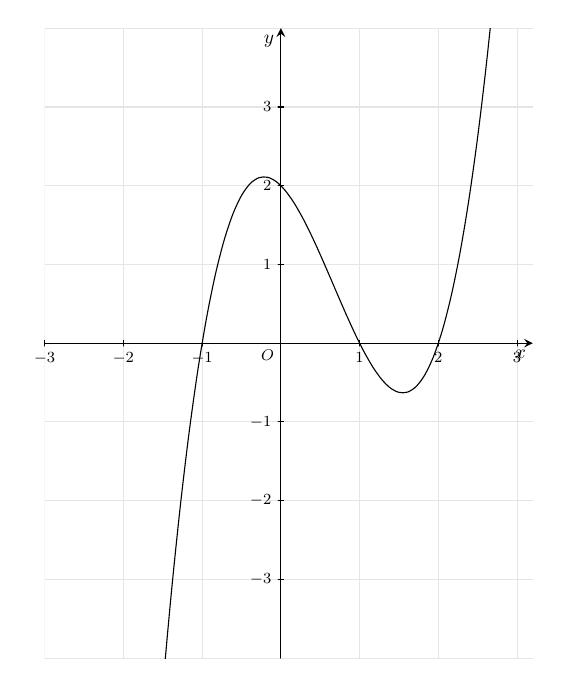
\begin{tikzpicture}[line join=round,line cap=round,>=stealth]
		\begin{scope}
			\clip (-3,-4)  rectangle (3.2,4);
			 \draw[gray!20](-4,-4) grid (4,4);
			\draw[samples=100,domain=-5.5:5.5,smooth,variable=\x] 
				 plot (\x,{(\x)^3+-2*(\x)^2+-(\x)+2});
		\end{scope}
		 \draw[->] (-3,0)--(3.2,0) node[below left] {$x$};
		 \draw[->] (0,-4)--(0,4) node[below left] {$y$};
		\draw (0,0) node  [below left] {\footnotesize $O$};
		\foreach \x  in {-3,-2,-1,1,2,3}
		\draw[thin] (\x,1pt)--(\x,-1pt) node [below]  {\footnotesize $\x$};
		\foreach \y in {-3,-2,-1,1,2,3} 
		\draw[thin] (1pt,\y)--(-1pt,\y) node [left] {\footnotesize  $\y$};
	\end{tikzpicture}
		}} 
	 \loigiai{
		Ta  có: $f'(x)=0\Leftrightarrow \hoac{&x=-1\\&x=1\\&x=2.}$\\
		Bảng  biên thiên
		\begin{center}
			
\begin{tikzpicture}
				 \tkzTabInit[nocadre,lgt=1,espcl=2]
					{$x$ /1,$y'$ /1,$y$ /2} 
					{$-\infty$,$-1$,$1$,$2$,$+\infty$} 
				 \tkzTabLine{,-,0,+,0,-,0,+}
				\tkzTabVar{+/$+\infty$,-/$f (-1)$,+/$f  (1)$,-/$f (2)$,+/$+\infty$}
			\end{tikzpicture}
		\end{center}
		 Dựa vào bảng biến thiên trên đoạn $[-1;2]$ hàm số có giá trị lớn nhất là $f(1)$.
	 }
\end{ex}

% từ: cau-hoi/lop12/2D1_Ung_dung_dao_ham_de_khao_sat_ham_so/2D1-2-1_Tim_cuc_tri_cua_ham_so_cho_boi_cong_thuc.tex
\begin{ex}%[2D1V2-1]%[ma:596d9238]
	Giá trị lớn  nhất của hàm số $f(x)=3x+\sin \dfrac{x}{2}$ trền đoạn $[0; 2\pi]$ là
	 \choice
		{\True  $6\pi$}
		{$7\pi$} 
		{$8\pi$} 
		 {$9\pi$}
	\loigiai{ 
		Ta có  $f'(x)=3+\dfrac{1}{2}\cos \dfrac{x}{2}=0$ (Phương trình vô nghiệm).\\
		Do đó $f'(x)>0,\forall x  \in [0;2\pi]$, nên hàm số đồng biến trên đoạn $[0;2\pi]$.\\
		Do  đó giá trị lớn nhất là $f(2\pi)=6\pi$.
	} 
\end{ex}

% từ: cau-hoi/lop12/2D1_Ung_dung_dao_ham_de_khao_sat_ham_so/2D1-2-7_Toan_thuc_te_ung_dung_cuc_tri_cua_ham_so.tex
\begin{bt}%[2D1V2-7]%[ma:f5527ce0]
	\immini{Một vật chuyển động với vận tốc $ v~( \text{ km/h})$ phụ thuộc vào thời gian $ t~( \text{ h})$ có đồ thị của hàm số dạng hàm bậc ba như hình bên. Biết rằng tại thời điểm $t_1=1~\text{ h}$ vật có vận tốc $v_1=4~\text{ km/h}$ và tại thời điểm $t_2=2~\text{ h}$ vật có vận tốc $v_2=1~\text{ km/h}$. Tính vận tốc của vật tại thời điểm $ t=3~\text{ h}$.}{\begin{tikzpicture}[scale=1,line join=round,line cap=round,>=stealth]
		\tikzset{ethicknode/.style={scale=1}} 
		 \def\xmin{-1}\def\xmax{3.5}\def\ymin{-1}\def\ymax{5}
		\draw[->] (\xmin-0.2,0)--(\xmax+0.2,0)  node[below]{$t$(h)};
		 \draw[->] (0,\ymin-0.2)--(0,\ymax+0.2) node[right]{$v$(km/h)};
		 \draw (0,0) node[below left]{$O$};
		\foreach  \x in {1,2}\draw (\x,0.1)--(\x,-0.1) node[below]{$\x$};
		\foreach \y  in {1,4}\draw (0.1,\y)--(-0.1,\y) node[left]{$\y$};
		\clip  (\xmin,\ymin) rectangle (\xmax,\ymax);
		\draw[smooth,samples=200,domain=\xmin:\xmax] plot  (\x,{6*((\x)^3)+-27*((\x)^2)+36*(\x)+-11});
		\draw[dashed] (1,0)--(1,4)--(0,4); \fill (1,4) circle (1.5pt); \fill (0,0)  circle (1.5pt);
		\draw[dashed] (2,0)--(2,1)--(0,1); \fill (2,1) circle (1.5pt); 
		\coordinate [label=above:$A$](A) at (1,4); 
		\coordinate [label=right:$B$](B)  at (2,1);
	\end{tikzpicture}
	} 
	\loigiai{ 
		Giả sử hàm số vận tốc  có dạng $ v( t)=at^3+bt^2+ct+d,$ $t>0$.\\
		 Ta có $v'( t)=3at^2+2bt+c$.\\
		Dựa vào đồ thị hàm số, tại các thời điểm $t_1$, $t_2$ đồ  thị hàm vận tốc đi qua các điểm cực trị $A( 1;4)$, $B( 2;1)$.\\
		Khi đó $$\heva{& v( 1)=4 \\ & v'( 1)=0 \\ & v(  2)=1 \\ & v'( 2)=0 }\Leftrightarrow \heva{& a+b+c+d=4 \\ & 3a+2b+c=0 \\ & 8a+4b+2c+d=1 \\ & 12a+4b+c=0 }\Leftrightarrow \heva{& a=6 \\ & b=-27 \\ & c=36 \\ & d=-11 .}$$
		Suy ra $  v( t)=6t^3-27t^2+36t-11$ (km/h).\\
	Vậy vận tốc của  vật tại thời điểm $ t=3$ h là $$ v( 3)=6\cdot 3^3-27\cdot 3^2+36\cdot 3-11=16~\text{ km/h}.$$}
\end{bt}

% từ: cau-hoi/lop12/2D1_Ung_dung_dao_ham_de_khao_sat_ham_so/2D1-3-1_GTLN_GTNN_tren_doan.tex
\begin{ex}%[2D1N3-1]%[ma:6e8be730]
	Cho $ac \neq 0$,$ad-bc\neq 0$. Đồ thị hàm số $y=\dfrac{ax+b}{cx+d}$ có đường  tiệm cận ngang là
	\choice 
		 {$x=\dfrac{a}{c}$}
		{$x=\dfrac{-d}{c}$} 
		{\True  $y=\dfrac{a}{c}$}
		 {$\mathrm{y}=\dfrac{-d}{c}$}
	\loigiai{ 
		Đồ  thị hàm số có tiệm cận ngang là $y=\dfrac{a}{c}$.
	} 
\end{ex}

% từ: cau-hoi/lop12/2D1_Ung_dung_dao_ham_de_khao_sat_ham_so/2D1-3-4_Ung_dung_GTNN_GTLN_trong_bai_toan_phuong_trin.tex
\begin{bt}%[2D1H3-4]%[ma:c1ba07a7]
% nguon: Archive/2024/TaiLieuGiangDay/1.HamSo/1. K12 - 4in1 - Hamso/ThubaiGoc/Bai3-Dang6.tex #2024
[Mức độ 2]%[BG12-4IN1, Nguyễn Khánh Trọng]
	Tìm tất cả giá trị của tham số $m$ để bất phương trình $x-m\le mx-3$ có nghiệm $x\in[0;3]$.
	\loigiai{
		Với $x\in[0;3]$, ta có 
		$$x-m\le mx-3\Leftrightarrow x+3\le mx+m\Leftrightarrow x+3\le m(x+1)\Leftrightarrow \dfrac{x+3}{x+1}\le m.$$
		Xét hàm số $f(x)=\dfrac{x+3}{x+1}$ trên đoạn $[0;3]$.\\
		Ta có $f'(x)=-\dfrac{2}{(x+1)^2}<0$, $\forall x\in[0;3]$ nên hàm số $f(x)$ luôn nghịch biến trên $(0;3)$.\\
		Suy ra $\min\limits_{[0;3]}f(x)=f(3)=\dfrac{3}{2}$.\\
		Khi đó, bất phương trình $x-m\le mx-3$ có nghiệm $x\in[0;3]$ khi và chỉ khi
		$$\min\limits_{[0;3]}f(x)\le m\Leftrightarrow m\ge \dfrac{3}{2}.$$
		Vậy $m\in\left[\dfrac{3}{2};+\infty\right)$.
	}	
\end{bt}

% từ: cau-hoi/lop12/2D1_Ung_dung_dao_ham_de_khao_sat_ham_so/2D1-4-1_Bai_toan_xac_dinh_cac_duong_tiem_can_cua_ham.tex
\begin{ex}%[2D1H4-1]%[ma:2909e870]
	 \immini
	{Cho hàm  số $y=f(x)$ có đồ thị như hình vẽ dưới đây. Đồ thị hàm số có đường tiệm cận xiên đi qua điểm nào dưới đây?
	 \choice
		{$M(1;2)$} 
		{$N(-2;1)$} 
		{\True $P(2;2)$} 
		{$Q(1;-1)$} 
		} 
		{\begin{tikzpicture}[scale=0.7,font=\footnotesize,line join=round,line cap=round,>=stealth]
		\def\xmin{-3}\def\xmax{3}\def\ymin{-4}\def\ymax{4} 
		\draw[->] (\xmin-0.2,0)--(\xmax+0.2,0)  node[below] {\footnotesize $x$};
		 \draw[->] (0,\ymin-0.2)--(0,\ymax+0.2) node[right] {\footnotesize $y$};
		\draw (0,0) node  [below right] {\footnotesize $O$};
		\foreach \x in {1}\draw (\x,0.05)--(\x,-0.05) node [below] {\footnotesize  $\x$};
		\foreach \x in {-1}\draw (\x,0.05)--(\x,-0.05) node [above]  {\footnotesize $\x$};
		\foreach \y in {1,2}\draw (0.05,\y)--(-0.05,\y) node [left] {\footnotesize $\y$}; 
		\foreach \y in {-2,-1}\draw (0.05,\y)--(-0.05,\y) node [right] {\footnotesize $\y$}; 
		\clip (\xmin,\ymin)  rectangle (\xmax,\ymax);
		\draw[dashed] (-0.0,\ymin)--(-0.0,\ymax); 
		\draw[dashed,domain=\xmin:\xmax] plot (\x,{1.0*(\x)+0.0}); 
		\draw[smooth,samples=200,domain=\xmin:-0.1] plot  (\x,{(1*((\x)^2)+0*(\x)+1)/(1*(\x)+0)});
		 \draw[smooth,samples=200,domain=0.1:\xmax] plot (\x,{(1*((\x)^2)+0*(\x)+1)/(1*(\x)+0)});
		 \draw[dashed] (-1.0,0)--(-1.0,-2.0)--(0,-2.0); \fill (-1.0,-2.0) circle (1pt);
		 \draw[dashed] (1.0,0)--(1.0,2.0)--(0,2.0); \fill (1.0,2.0) circle (1pt);
		\draw[dashed] (-1.0,-1.0)--(0,-1.0); 
		\draw[dashed]  (1.0,1.0)--(0,1.0);
	\end{tikzpicture}
		 }
	\loigiai{Đường tiệm cận  xiên trong đồ thị hàm số có dạng là một đường thẳng đi qua $3$ điểm là $O(0; 0)$, $(-1; -1)$, $(1; 1)$.\\
		Gọi $(C) \colon y=ax+b$  là hàm số biểu diễn đường tiệm cận xiên $\Rightarrow y=x$.\\
		Vậy đường  tiệm cận xiên của đồ thị hàm số đi qua điểm $P(2; 2)$.
	 }
\end{ex}

% từ: cau-hoi/lop12/2D1_Ung_dung_dao_ham_de_khao_sat_ham_so/2D1-4-2_Bai_toan_xac_dinh_cac_duong_tiem_can_cua_ham.tex
\begin{ex}%[2D1H4-2]%[ma:d38d7da5]
	Cho hàm số $y=f(x)=\dfrac{nx^2+1}{mx+1} (mn\neq 0)$  có đồ thị $(C)$ như hình vẽ:
	\begin{center}
		\begin{tikzpicture}[scale=1,font=\footnotesize,line join=round,line cap=round,>=stealth]
			\def\a{1} \def\b{0} \def\c{1} \def\d{2} \def\e{1} 
			\def\xmin{-6}  \def\xmax{5}
			\def\ymin{-5}  \def\ymax{5}
			\draw[->] (\xmin,0)--(\xmax,0) node [below]{$x$}; 
			 \draw[->] (0,\ymin)--(0,\ymax) node [right]{$y$};
			 \node at (0,0) [above right]{$O$};
			\clip (\xmin+0.1,\ymin+0.1) rectangle (\xmax-0.1,\ymax-0.1); 
			 \draw[smooth,samples=300,domain=\xmin:(-\e/\d-0.1)] plot (\x,{(\a*(\x)^2+\b*(\x)+\c)/(\d*(\x)+\e)});
			\draw[smooth,samples=300,domain=(-\e/\d+0.1:\xmax)] plot (\x,{(\a*(\x)^2+\b*(\x)+\c)/(\d*(\x)+\e)}); 
			\draw[smooth,samples=300,domain=\xmin:\xmax] plot (\x,{(0.5*(\x)-0.25)}); 
			\draw  (-\e/\d,\ymin)--(-\e/\d,\ymax);
			\fill (-0.5,0) circle (1.0pt) node[above  left]{$-\dfrac{1}{2}$};
			\node at  (-4.1,-1)[below]{$y=\dfrac{1}{2}x-\dfrac{1}{4}$};
		\end{tikzpicture}
	\end{center}
	\choiceTF 
		 {$\dfrac{n}{m}=-\dfrac{1}{4}$}
		 {$m=-\dfrac{1}{2}$}
		 {\True $m+n=3$}
		{$\lim\limits_{x\to+\infty}\left[f(x)-\dfrac{1}{2}x\right]=0$} 
	\loigiai{ 
		\begin{itemchoice}
			\itemch $\lim\limits_{x\to+\infty}\dfrac{f(x)}{x}=\lim\limits_{x\to+\infty}\dfrac{nx^2+1}{mx^2+x}=\dfrac{n}{m}=\dfrac{1}{2}$. 
			\itemch Đường tiệm cận đứng của đồ thị là $x=-\dfrac{1}{m}=-\dfrac{1}{2}\Rightarrow m=2$. 
			\itemch Từ hai ý a) và b) ta có $\heva{&m=2n\\&m=2}\Rightarrow\heva{&m=2\\&n=1}\Rightarrow  m+n=3$; $n=2\Rightarrow m+n=3$.\\
			\itemch Đường  tiệm cận xiên $y=\dfrac{1}{2}x-\dfrac{1}{4}\Rightarrow\lim\limits_{x\to+\infty}\left[f(x)-\dfrac{1}{2}x\right]=-\dfrac{1}{4}$.
		\end{itemchoice}
	 }
\end{ex}

% từ: cau-hoi/lop12/2D1_Ung_dung_dao_ham_de_khao_sat_ham_so/2D1-5-1_Nhan_dang_do_thi.tex
\begin{ex}%[2D1V5-1]%[ma:641a4539]
	Cho hàm số $y=\dfrac{x-1}{x+1}$ có đồ  thị $\left( C \right)$.
	 \choiceTF
		{\True Đạo hàm  hàm số là $y'=\dfrac{2}{\left( x+1 \right)^2}$}
		{\True Tiệm cận ngang của đồ thị hàm số  là $y=1$}
		{Tâm đối xứng của đồ thị hàm số  là $\left( 1;-1 \right)$}
		{Với mọi $M\in \left( C \right)$, tích khoảng cách từ $M$  đến các đường tiệm cận bằng $3$}
	 \loigiai{
		\begin{itemchoice}
			 \itemch {\bf Đúng.}\\
			Đạo hàm hàm  số là $y'=\dfrac{2}{\left( x+1 \right)^2}$.
			\itemch {\bf Đúng.}\\ 
			Tiệm cận ngang của đồ thị hàm số là $y=1$. 
			 \itemch {\bf Sai.}\\
			Tâm đối xứng của đồ thị hàm số  $\left( -1;1 \right)$.
			\itemch {\bf  Sai.}\\
			 Gọi $M\left( x_0;y_0 \right)\in \left( C \right)\Rightarrow M\left( x_0;1-\dfrac{2}{x_0+1} \right)$.\\
			 Khoảng cách từ $M$ đến tiệm cận đứng: $d_1=\left| x_0+1 \right|$.\\
			Khoảng cách từ $M$ đến tiệm cận ngang: $d_2=\left| y_0-1 \right|=\left| 1-\dfrac{2}{x_0+1}-1 \right|=\dfrac{2}{\left| x_0+1 \right|}$.\\ 
			Vậy $d_1\cdot  d_2=2$.
	\end{itemchoice}}
\end{ex}

% từ: cau-hoi/lop12/2D1_Ung_dung_dao_ham_de_khao_sat_ham_so/2D1-5-6_Phuong_trinh_tiep_tuyen_cua_do_thi_ham_so.tex
\begin{ex}%[2D1H5-6]%[ma:2b6ed5e8]
	Cho hàm số $y= x^3-2x+ 1.$ Viết phương trình  tiếp tuyến của đồ thị hàm số tại điểm $M(0;1)$.
	 \choice
		{$ y=2x  +3$}
		{\True $ y=-2x + 1$} 
		{$ y=4x + 1$} 
		{$ y=-4x + 1$} 
	\loigiai{ 
		Đạo hàm của hàm số đã cho là $y'= 3x^2-2$ $\Rightarrow$ $y'(0)=-2$.\\ 
		Phương trình tiếp tuyến của đồ thị hàm số tại điểm $M(0;1)$  là\\
		$y-1=  -2(x-0)$ hay $ y=-2x + 1$.
	} 
\end{ex}

% từ: cau-hoi/lop12/2D1_Ung_dung_dao_ham_de_khao_sat_ham_so/2D1-5-7_Diem_dac_biet_cua_do_thi_ham_so.tex
\begin{bt}%[2D1V5-7]%[ma:02de6435]
	Cho hàm số $(C_m)\colon  y=\dfrac{x^2+2mx+2}{x+1}=x+2m-1+\dfrac{3-2m}{x+1}$.\\
	Tìm các giá trị của $m$ để hàm số có cực đại, cực tiểu  và khoảng cách giữa hai điểm đó tới đường thẳng $d: x+y+2=0$ bằng nhau.
	\loigiai{ 
		Tập  xác định: $\mathscr{D}=\mathbb{R}\setminus\{-1\}$.\\
		Ta có $y'=\dfrac{x^2+2x+2m-2}{(x+1)^2}$. Khi  đó $y'=0\Leftrightarrow x^2+2x+2m-2=0\, (*)$.\\
		Hàm  số có cực đại và cực tiểu khi và chỉ khi $(*)$ có hai nghiệm phân biệt khác $-1$.\\
		Tương đương $\heva{&\triangle'=3-2m>0\\&(-1)^2+2(-1)+2m-2\neq0}\Leftrightarrow\heva{&m<\dfrac{3}{2}\\&m\neq\dfrac{3}{2}}\Leftrightarrow m<\dfrac{3}{2}$\,  (1).\\
		Gọi $A(x_1; y_1);  B(x_2; y_2)$ lần lượt là hai điểm cực trị của hàm số với $x_1, x_2\neq-1$ là hai nghiệm của phương trình $(*)$.\\
		Áp dụng định lí Vi-et, ta  có $\heva{&x_1+x_2=-2\\&x_1\cdot x_2=2m-2.}$\\
		Mặt khác đường thẳng đi qua  hai điểm cực trị có phương trình là $y=2x+m$ cho nên $y_1=2x_1+m; y_2=2x_2+m\Rightarrow A(x_1; 2x_1+m); B(x_2; 2x_2+m)$.\\
		Theo giả thiết ta có  $\dfrac{|x_1+y_1+2|}{\sqrt{2}}=\dfrac{|x_2+y_2|}{\sqrt{2}}\Rightarrow|x_1+y_1+2|=|x_2+y_2+2|$.\\
		Tương đương 
		\begin{align*}
			&\, |3x_1+2m+2|=|3x_2+2m+2| 
			 \Leftrightarrow (3x_1+2m+2)^2-(3x_2+2m+2)^2=0\\
			 \Leftrightarrow&\, (x_1-x_2)\left[3(x_1+x_2+4m+4)\right]=0\\
			\Leftrightarrow&\, 3(x_1+x_2+4m+4)=0 (x_1\neq x_2)\Leftrightarrow  3(-2+4m+4)=0\\
			\Rightarrow&\, m=-\dfrac{1}{2} \,  \text{ thỏa mãn điều kiện} (*).
		\end{align*}
		Vậy giá trị $m$ cần tìm là  $m=-\dfrac{1}{2}$.
	 }
\end{bt}

% từ: cau-hoi/lop12/2D1_Ung_dung_dao_ham_de_khao_sat_ham_so/2D1-5-8_Toan_thuc_te_ung_dung_khao_sat_ham_so.tex
\begin{ex}%[2D1V5-8]%[ma:7c90497f]
% nguon: Archive/2024/San pham - To Latex Strong - Tex hoa Lop 12 moi - Dot 1 (Chuong 1)/San pham - To Latex Strong - Tex hoa Lop 12 moi - Dot 1 (Chuong 1)/Data/Ket noi tri thuc/To 16 - Dot 16 - Chuong 1 - Bai 5 - KNTT - De 1.tex #945
%[Tổ 16 - Đợt 16 - Chương 1 - Bài 5 - KNTT]%[Võ Thị Thùy Trang]
	Một chất điểm chuyển động theo phương trình $s(t)=t^3-3t^2+8t+1$, trong đó $t$ tính bằng giây và $s(t)$ tính bằng mét. Khi đó
	\choiceTF
	{Vận tốc của chất điểm tại thời điểm $t=3$ (s) bằng $8$ m/s}
	{\True Tại thời điểm mà chất điểm di chuyển được $13$ m , vận tốc khi đó bằng $8$ m/s}
	{\True Vận tốc nhỏ nhất của chất điểm là $5$ m/s}
	{Gia tốc tại thời điểm chất điểm đạt vận tốc nhỏ nhất bằng $2$ m/s$^2$}
	\loigiai
	{
		\begin{itemchoice}
			\itemch \textbf{Sai}. Vận tốc $v(t)=3t^2-6t+8$.\\
			Vận tốc của chất điểm tại thời điểm $t=3$ s bằng $v(3)=17$ m/s.
			\itemch\textbf{ Đúng}. Chất điểm di chuyển được $13$ m $\Leftrightarrow t^3-3t^2+8t+1=13 \Leftrightarrow t=2$ (s).\\
			Vận tốc khi đó bằng $v(2)=8$ m/s.
			\itemch \textbf{Đúng}. Vận tốc $v(t)=3t^2-6t+8$.\\
			$v'(t)=6 t-6 \Leftrightarrow t=1$.\\
			Bảng biến thiên
			\begin{center}
				
\begin{tikzpicture}[>=stealth,line join=round,line cap=round,font=\footnotesize,scale=1]
					\tkzTabInit[nocadre=false,lgt=1,espcl=2,deltacl=0.5]{$t$/.7 ,$v'$/.7,$v$/2}
					{$0$ , $1$ , $+\infty$}
					\tkzTabLine{ , - , $0$ , + , }
					\tkzTabVar{+/$$ , -/$5$ , +/$$}
				\end{tikzpicture}
			\end{center}
			Vận tốc nhỏ nhất bằng $5$ m/s tại thời điểm $t=1$ (s).
			\itemch \textbf{Sai}. Gia tốc $a(t)=6t-6$.
			Gia tốc tại thời điểm $t=1$ (s) bằng $a(1)=0$.
		\end{itemchoice}
	}
\end{ex}

% từ: cau-hoi/lop12/2D1_Ung_dung_dao_ham_de_khao_sat_ham_so/2D1-5-8_Toan_thuc_te_ung_dung_khao_sat_ham_so.tex
\begin{bt}%[2D1C5-8]%[ma:9c0700b2]
% nguon: Archive/2024/San pham - To Latex Strong - Tex hoa Lop 12 moi - Dot 3 (Chuong 1 + 2 +3 + 4)/Data/Chuong 1/Ket noi tri thuc/To 15 - Dot 16 - Chuong 1 - Bai 4 - KNTT - De 3.tex #3514
%[Tổ 15 - Đợt 16 - Chương 1 - Ôn tập chương 1 - KNTT - Đề 3]%[Tex hóa: Lê Thị Thúy Hằng]
	Bác An có một mảnh đất ruộng và muốn dành ra một khu đất hình chữ nhật có diện tích $242$ m$^2$ để trồng cây thuốc. Bác dự kiến rào quanh ba cạnh của khu đất hình chữ nhật này bằng lưới thép, cạnh còn lại (chiều dài) sẽ tận dụng bức tường có sẵn. Biết chiều rộng khu đất không vượt quá $16$ m. Hỏi chiều rộng của khu đất bằng bao nhiêu để tổng chiều dài lưới thép cần dùng là ngắn nhất (nghĩa là chi phí rào lưới thép thấp nhất)?
	\shortans{$11$}
	\loigiai{
		%FB tác giả: Nguyễn Thị Hồng Nhung\\
		%FB phản biện:Nguyễn Thị Thanh Nguyệt\\
		Gọi chiều rộng khu đất hình chữ nhật cần rào là $x$ (m), $0< x \le 16$.\\
		Diện tích khu đất này là $242$ m$^2$ nên chiều dài của khu đất là 
		$\dfrac{242}{x}$ (m)\\
		Tổng chiều dài lưới thép rào quanh khu đất hình chữ nhật là $2x+\dfrac{242}{x}$ (m).\\
		Xét hàm số $y=2x+\dfrac{242}{x}$, $x \in \left( 0; 16 \right]$.\\
		Ta có $y'=2-\dfrac{242}{x^2} = \dfrac{2x^2-242}{x^2}$ và $y'=0 \Leftrightarrow 2x^2-242=0 \Rightarrow x=11$ (do $x \in \left( 0; 16 \right]$).\\
		Ta có
		$\lim\limits_{x \to 0^+} y = \lim\limits_{x \to 0^+} \left( 2x + \dfrac{242}{x} \right) = +\infty$; $y(11)=44$; $y(16)=\dfrac{377}{8}$.\\
		Bảng biến thiên
		\begin{center}
			
\begin{tikzpicture}
				\tkzTabInit[espcl=2.5,lgt=1.5]
				{$x$/0.7,$y'$/0.7,$y$/2.1}
				{$0$,$11$,$16$}
				\tkzTabLine{,-,0,+}
				\tkzTabVar{+/$+\infty$,-/$44$,+/$\dfrac{377}{8}$}
			\end{tikzpicture}
		\end{center}
		Dựa vào bảng biến thiên, chiều dài lưới thép ngắn nhất là $44$ m khi chiều rộng khu đất là $11$ m.\\
	}
\end{bt}

% từ: cau-hoi/lop12/2D3_Cac_so_dac_trung_ghep_nhom/2D3-1-1_Cong_thuc_ly_thuyet.tex
\begin{bt}%[2D3H1-1]%[ma:af16dbc2]
	Biết hàm số $F(x)=\dfrac{2 x^2-3 x+6}{x}$ là một nguyên hàm của hàm  số $$f(x)=\dfrac{a x^2+b x+c}{x^2} \quad \text{ (với $a$, $b$, $c$ là các số thực)}.$$
	Khi đó  giá trị $a+b-c$ bằng bao nhiêu?
	\shortans{8} 
	 \loigiai{
		Ta có $F'(x)=\left(2 x-3+\dfrac{6}{x}\right)'=2-\dfrac{6}{x^2}=\dfrac{2 x^2-6}{x^2}$  và $F'(x)=f(x)$.
		\\ 
		Suy ra $a=2$; $b=0$; $c=-6$. Do  đó $a+b-c=8$.
	 }
\end{bt}

% từ: cau-hoi/lop12/2D3_Cac_so_dac_trung_ghep_nhom/2D3-1-1_Cong_thuc_ly_thuyet.tex
\begin{bt}%[2D3B1-1]%[ma:8a39cad2]
	Cho hàm  số $f(x) = x\sqrt{x}$ có một nguyên hàm là $F(x)$ thỏa $F(1) = 3$. Tính $F(4)$.
	 \shortans{15,4}
	 \loigiai{
		Ta có $F(x)=\displaystyle \int  x\sqrt{x}\mathrm{\,d}x=\displaystyle \int x^{\frac{3}{2}}\mathrm{\,d}x=\dfrac{2}{5}x^{\frac{5}{2}}+C$.\\
		Mà $F(1)=3\Rightarrow  \dfrac{2}{5}+C=3\Rightarrow C =\dfrac{13}{5}$.\\
		 Do đó $F(x)=\dfrac{2}{5}x^{\frac{5}{2}}+\dfrac{13}{5}$.\\
		Vậy  $F(4)=\dfrac{77}{5}=15{,}4$.
	 }
\end{bt}

% từ: cau-hoi/lop12/2D4_Nguyen_ham_tich_phan/2D4-1-2_Nguyen_ham_co_ban_da_thuc_phan_thuc.tex
\begin{ex}%[2D4H1-2]%[ma:9f206a3a]
	 Biết rằng $\displaystyle\int_{0}^{2}f(x)\mathrm{\,d}x=-4$. Giá trị của $\displaystyle\int_{0}^{2}[3x-2f(x)]\mathrm{\,d}x$ bằng
	\choice 
		{$-2$} 
		 {$12$}
		{\True $14$} 
		{$22$} 
	\loigiai{ 
		 Ta có $\displaystyle\int_{0}^{2}[3x-2f(x)]\mathrm{\,d}x=\displaystyle\int_{0}^{2}3x\mathrm{\,d}x-2\displaystyle\int_{0}^{2}f(x)\mathrm{\,d}x=\left(\dfrac{3x^2}{2}\right)\bigg|_{0}^{2}-2(-4)=6+8=14$
	 }
\end{ex}

% từ: cau-hoi/lop12/2D4_Nguyen_ham_tich_phan/2D4-1-6_Toan_thuc_te_ap_dung_nguyen_ham.tex
\begin{bt}%[2D4V1-6]%[ma:ecc3f687]
% nguon: Archive/SP-4Phan-Dot3/Data/CTST_2-OTGK2-De02.tex #4528

Người ta trồng hoa vào phần đất được tô màu đen được giới hạn bởi cạnh $AB$, $CD$  đường trung bình  $MN$ của mảnh đất hình chữ nhật  $ABCD$ và một đường cong hình sin (như hình vẽ). Biết $AB=2\pi$ (m), $AD=2$ (m). Tính diện tích phần đát còn lại.
	\begin{center}
	\begin{tikzpicture}[scale=1,>=stealth, font=\footnotesize, line join=round, line cap=round]
		\path 
		(-pi,1) coordinate (A)
		(pi,1) coordinate (B)
		(pi,-1) coordinate (C)
		(-pi,-1) coordinate (D)
		(-pi,0) coordinate (M)
		(pi,0) coordinate (N)
		;
		\draw (A)--(B)--(C)--(D)--cycle (M)--(N);
		\draw[smooth,samples=400,domain=-pi:pi] plot(\x,{sin(\x r)});
		\fill[pattern= north east lines] plot[domain=-pi:pi ](\x,{sin(\x r)});
		\foreach \x/\g in {A/150,B/30,C/-30,D/-150,M/180,N/0}
		\fill[black] 	(\x) circle (1pt)
		($(\g:3mm)+(\x)$) node {$\x$};
	\end{tikzpicture}
\end{center}
	\loigiai{
		\begin{center}
		\begin{tikzpicture}[scale=1,>=stealth, font=\footnotesize, line join=round, line cap=round]
			\path 
			(-pi,1) coordinate (A)
			(pi,1) coordinate (B)
			(pi,-1) coordinate (C)
			(-pi,-1) coordinate (D)
			(-pi,0) coordinate (M)
			(pi,0) coordinate (N)
			;
			\draw[->] (-4,0)--(4,0) node[below right]{$x$};
			\draw[->] (0,-1.5)--(0,1.5) node[left]{$y$};
			\node[below right] at (0,0) {$O$};
			\draw (A)--(B)--(C)--(D)--cycle (M)--(N);
			\draw[smooth,samples=400,domain=-pi:pi] plot(\x,{sin(\x r)});
			\fill[pattern= north east lines] plot[domain=-pi:pi ](\x,{sin(\x r)});
			\foreach \x/\g in {A/150,B/30,C/-30,D/-150,M/135,N/45}
			\fill[black] 	(\x) circle (1pt)
			($(\g:3mm)+(\x)$) node {$\x$};
		\end{tikzpicture}
		\end{center}
		Chọn hệ trục tọa độ $Oxy$ như hình vẽ. Khi đó\\
		Diện tích hình chữ nhật $ABCD$ bằng $S_1=AB\cdot AD=4\pi$.\\
		Diện tích phần đất trồng hoa bằng
		$$S_2=2\displaystyle\int\limits_{0}^{\pi} \sin x \mathrm{\,d}x 
		= -2\cos x \Big|_{0}^{\pi}
		= -2\left(\cos 0 - \cos\pi\right)=4.$$
		Suy ra phần đất còn lại bằng $S=S_1-S_2=4\pi -4 =4(\pi -1)$ m$^2$.
	}
\end{bt}

% từ: cau-hoi/lop12/2D4_Nguyen_ham_tich_phan/2D4-2-6_Toan_thuc_te_ap_dung_nguyen_ham.tex
\begin{bt}%[2D4V2-6]%[ma:72440f87]
	Trên một tuyến đường thẳng có một đoạn phải đi xuyên qua một quả núi nhỏ, do đó người ta đã tạo một hằm chui để thuận tiện  cho các phương tiện giao thông di chuyển, vòm của hầm chui được đổ bê tông có dạng như hình vẽ dưới đây với $BC=8$ m; $IH=5$ m; $IK=0{,}6$ m; $AB=CD=0{,}5$ m; $HT=10$ m. Biết khi cắt vòm của hầm chui bằng mật phẳng vuông góc với trục của tuyến đường ta luôn có thiết diện là một hình phẳng được giới hạn bởi hai parabol và giao tuyến của mặt cắt với mặt đường. Hỏi cần bao nhiêu mét khối bê tông để đổ vòm của hầm chui (làm tròn kết quả đến hàng phần mười).
	\begin{center}
		\begin{tikzpicture}[line join=round,line cap=round,>=stealth]
				\tikzset{every node/.style={scale=0.7}} 
				\draw[->]  (-5.1,0)--(13,0) node[below left] {};
				\draw[->] (0,-1.1)--(0,14) node[left] {}; 
				\draw (0,0) node  [below left] {$H$};
				\begin{scope}
					 \clip (-5,-1) rectangle (14,14);
					\fill[red!40,opacity=0.6] 
						plot[domain=-4.5:4.5,samples=300] (\x,{-112/405*(\x)^2+5.6}) 
						-- plot[domain=4:-4,samples=300]  (\x,{-5/16*(\x)^2+5})
						 -- cycle;
					 \fill[gray!40,opacity=0.6]
						 plot[domain=4:-4,samples=300] (\x,{-5/16*(\x)^2+5});
					\draw[blue,samples=300,domain=-4.5:4.5,smooth,variable=\x] 
						plot (\x,{-112/405*(\x)^2+5.6}) node[right,scale=0.8]  {};
					\draw[red,samples=300,domain=-4:4,smooth,variable=\x] 
						 plot (\x,{-5/16*(\x)^2+5}) node[right,scale=0.8] {};
					\draw[dashed,blue!70!black,samples=300,domain=2.5:5,smooth,variable=\x] 
						plot  (\x,{-112/405*(\x-7)^2+5.6+7}) node[right,scale=0.8] {};
					\draw[blue!70!black,samples=300,domain=5:11.5,smooth,variable=\x] 
						plot (\x,{-112/405*(\x-7)^2+5.6+7}) node[right,scale=0.8] {}; 
					\draw[dashed,red!70!black,samples=300,domain=3:11,smooth,variable=\x] 
						plot (\x,{-5/16*(\x-7)^2+5+7})  node[right,scale=0.8] {};
				\end{scope}
				\coordinate  (A) at (-4.5,{-112/405*(-4.5)^2+5.6});
				 \coordinate (D) at (4.5,{-112/405*(4.5)^2+5.6});
				\coordinate (V1) at (-2,364/81); 
				\coordinate (A') at  ($(A)+(7,7)$);
				\coordinate (D')  at ($(D)+(7,7)$);
				 \coordinate (V1') at ($(V1)+(7,7)$);
				 \coordinate (B) at (-4,{-5/16*(-4)^2+5});
				\coordinate (C)  at (4,{-5/16*(4)^2+5});
				\coordinate (V2)  at (0,5);
				\coordinate (V3) at (0,5.6); 
				\coordinate (B')  at ($(B)+(7,7)$);
				\coordinate (C')  at ($(C)+(7,7)$);
				 \coordinate (V2') at ($(V2)+(7,7)$);
				\coordinate (H)  at (0,0);
				\coordinate (T) at  ($(H)+(7,7)$);
				\draw[gray,dashed] (A)--(A'); 
				\draw (D)--(D'); 
				\draw (V1)--(V1'); 
				\draw[gray,dashed]  (B)--(B');
				\draw[gray,dashed] (C)--(C'); 
				\draw[dashed]  (A')--(D');
				 \draw[dashed] (H)--(T);
				\node at (T)  [above right]{$T$};
				\node at (A) [below]{$A$}; 
				\node at (B) [below]{$B$}; 
				\node at  (C) [below]{$C$};
				 \node at (D) [below]{$D$};
				\node at (D)  [below]{$D$};
				\node at (V2) [below left]{$I$}; 
				\node at (V3)  [above right]{$K$};
				\foreach \p/\pos in {V1/above  left,V1'/above right,
					A/below left,A'/above  right,
					D/below right,D'/above right, 
					V2/above left,V2'/above  right,
					B/below left,B'/above right, 
					 C/below right,C'/above right}{
					\fill  (\p) circle (1.5pt);
				 }
				\fill[orange!40,opacity=0.6] 
					(V1)--plot[domain=-2:4.5,samples=300]  (\x,{-112/405*(\x)^2+5.6})
					 (D)--(D')--plot[domain=11.5:5,samples=300] (\x,{-112/405*(\x-7)^2+5.6+7})--(V1')--(V1);
			\end{tikzpicture}
	\end{center}
	\shortans{69,3} 
	\loigiai{ 
		\begin{center}
			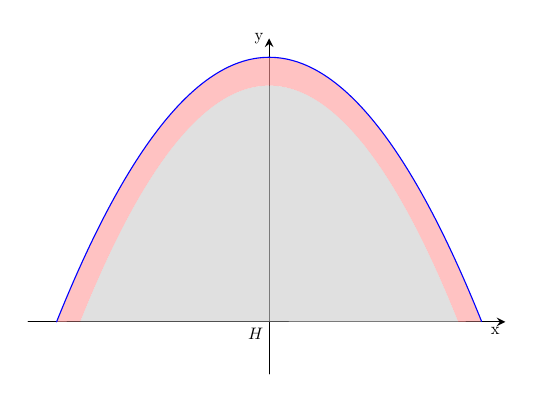
\begin{tikzpicture}[line join=round,line cap=round,>=stealth,scale=0.6]
					\tikzset{every  node/.style={scale=0.6}}
					\draw[->] (-5.1,0)--(5,0)  node[below left] {x};
					\draw[->] (0,-1.1)--(0,6) node[left]  {y};
					\draw (0,0) node [below left] {$H$}; 
					\fill[red!40,opacity=0.6] 
						plot[domain=-4.5:4.5,samples=300]  (\x,{-112/405*(\x)^2+5.6})
						 -- plot[domain=4:-4,samples=300] (\x,{-5/16*(\x)^2+5})
						--  cycle;
					\fill[gray!40,opacity=0.6] 
						 plot[domain=4:-4,samples=300] (\x,{-5/16*(\x)^2+5});
					 \draw[blue,samples=300,domain=-4.5:4.5,smooth,variable=\x]
						plot  (\x,{-112/405*(\x)^2+5.6}) node[right,scale=0.8] {};
				\end{tikzpicture}
		\end{center}
		Gọi $S$ là diện tích hình phẳng giới hạn bởi hai parabol  và giao tuyến của mặt cắt với mặt đường.\\
		Thể tích vòm của  hầm chui được đổ bê tông là $V=S \cdot HT=10S$.\\
		 Gắn phần diện tích vào hệ trục tọa độ $Oxy$, ta có đồ thị như hình vẽ.\\
		Từ đồ thị,  ta xác định được hai hàm số parabol:\\
		$g(x)=k\left(x^2-\dfrac{81}{4}\right) \xrightarrow{g(0)=\dfrac{28}{5}} k=-\dfrac{112}{405} \Rightarrow  g(x)=-\dfrac{112}{405}\left(x^2-\dfrac{81}{4}\right)$\\
		 $f(x)=h(x^2-16) \Rightarrow h=-\dfrac{5}{16} \Rightarrow f(x)=-\dfrac{5}{16}(x^2-16).$\\
		$\Rightarrow S=\displaystyle\int_{-\sqrt{3}}^{\sqrt{3}} \left(g(x)-f(x)\right) \mathrm{\,d}x=\displaystyle\int_{-\sqrt{3}}^{\sqrt{3}}  \left[-\dfrac{112}{405}\left(x^2-\dfrac{81}{4}\right)-\left(-\dfrac{5}{16}(x^2-16)\right)\right] \mathrm{\,d}x=\dfrac{104}{15}.$\\
	Vậy thể tích của vòm là \[V=\dfrac{104}{15} \cdot 10=\dfrac{208}{3} \approx  69,3(\text{m}^3).\]}
\end{bt}

% từ: cau-hoi/lop12/2D4_Nguyen_ham_tich_phan/2D4-2-6_Toan_thuc_te_ap_dung_nguyen_ham.tex
\begin{bt}%[2D4V2-6]%[ma:a2a6b2ab]
	\immini 
	{Hai hàm  số $y = f(x)$; $y = g(x)$ đều là những hàm số bậc hai có đồ thị như hình vẽ bên cạnh. Tính diện tích phần tô đậm (\textit{làm tròn đến hai chữ số thập phân}).
	} 
	{\begin{tikzpicture}[>=stealth,line join=round,line cap=round,color=blue,font=\footnotesize,scale=0.8]
		\draw[->]  (-2,0) -- (5,0) node[below] {$x$};
		\draw[->] (0,-1)--(0,5)  node[right]{$y$};
		 \draw (0,0) node[below left]{$O$};
		\draw (-1,0)  node[above left]{$-1$}
			 (4,0) node[above right]{$4$}
			 (0,3) node[left]{$3$}
			(0,2)  node[right]{$2$};
		\fill[pattern  = north east lines,pattern color=cyan,smooth] plot[domain=-1:4] (\x,{-0.75*((\x)+1)*((\x)-4)})--plot[domain=4:-1] (\x,{-0.5*((\x)+1)*((\x)-4)})--cycle;
		\draw[violet,samples=150,smooth,domain=-1.3:4.3] plot  (\x,{-0.5*((\x)+1)*((\x)-4)});
		\draw[violet,samples=150,smooth,domain=-1.2:4.2] plot  (\x,{-0.75*((\x)+1)*((\x)-4)});
		 \draw (3.2,3.6) node[above]{\scriptsize $y = f (x)$};
		 \draw (2.45,1.4) node[above]{\scriptsize $y = g (x)$};
	\end{tikzpicture}
	} 
	 \shortans{5,21}
	 \loigiai{
		Vì hàm số  $y = f(x)$ là hàm số bậc hai và đồ thị $y = f(x)$ cắt trục $Ox$ tại các điểm có hoành độ $-1$ và $4$ nên $f(x) = a(x + 1)(x - 4)$.\\
		 Đồ thị $y = f(x)$ đi qua điểm $(0; 3)$ nên $a = -\dfrac{3}{4} \Rightarrow f(x) = -\dfrac{3}{4}(x+1)(x-4)$.\\
		Tương tự $g(x) =  -\dfrac{1}{2}(x+1)(x-4)$.\\
		Do đó diện tích phần tô đậm bằng $\displaystyle\int_{-1}^4 \left[\dfrac{-3}{4}(x+1)(x-4) + \dfrac{1}{2}(x+1)(x-4)\right] \mathrm{\,d}x = \dfrac{125}{24} \approx  5{,}21$.
	 }
\end{bt}

% từ: cau-hoi/lop12/2D4_Nguyen_ham_tich_phan/2D4-2-6_Toan_thuc_te_ap_dung_nguyen_ham.tex
\begin{bt}%[2D4V2-6]%[ma:7d3f575c]
	Cho hình vẽ dưới đây là đồ thị vận tốc $v(t)$ của một vật ($t=0$ là thời điểm vật  bắt đầu chuyển động). Tính vận tốc trung bình (m/s) của vật $10$ giây đầu tiên.
	\begin{center}
		\begin{tikzpicture}[scale=1,font=\footnotesize,line join=round,line cap=round,>=stealth]
				\def\xmin{-1};  \def\ymin{-1}; \def\xmax{11}; \def\ymax{5};
				\coordinate  (O) at (0,0);
				\draw[->] (\xmin,0)--(\xmax,0) node[below]{$x$}; 
				\draw[->] (0,\ymin)--(0,\ymax) node[left]{$y$}; 
				\fill (O) node[below left]{$O$}  circle (1pt);
				 \clip ({\xmin-0.1},{\ymin-0.1}) rectangle ({\xmax+0.1},{\ymax+0.1});
				\foreach  \x in {2,4,7,10}{
					\fill (\x,0) node[below]{$\x$} circle  (1pt);
				 }
				\foreach  \y in {1,3}{
					 \fill (0,\y) node[left]{$\y$} circle (1pt);
				} 
				 \draw (0,0)--(2,1)--(4,3)--(7,3)--(10,1);
				 \draw[dashed] (2,0)|-(0,1)
					(4,0)|-(0,3) 
					 (7,0)--(7,3)
					(10,0)|-(0,1); 
			\end{tikzpicture}
	\end{center}
	\shortans{2} 
	 \loigiai{
		 Theo đồ thị ta có
		\begin{center}
			\begin{tikzpicture}[scale=1,font=\footnotesize,line join=round,line cap=round,>=stealth]
					\def\xmin{-1}; \def\ymin{-1}; \def\xmax{11};  \def\ymax{5};
					\coordinate  (O) at (0,0);
					 \draw[->] (\xmin,0)--(\xmax,0) node[below]{$x$};
					\draw[->] (0,\ymin)--(0,\ymax)  node[left]{$y$};
					\fill (O) node[below left]{$O$} circle (1pt); 
					\clip ({\xmin-0.1},{\ymin-0.1})  rectangle ({\xmax+0.1},{\ymax+0.1});
					\foreach \x in {2,4,7,10}{ 
						\fill  (\x,0) node[below]{$\x$} circle (1pt);
					 }
					\foreach \y  in {1,3}{
						\fill (0,\y) node[left]{$\y$} circle  (1pt);
					 }
					\draw (0,0)--(2,1) node[above]{$B$}--(4,3) node[above]{$C$}--(7,3) node[above]{$D$}--(10,1) node[above]{$E$}; 
					\draw[dashed] (2,0)|-(0,1) 
						 (4,0)|-(0,3)
						 (7,0)--(7,3)
						 (10,0)|-(0,1);
				\end{tikzpicture}
		\end{center}
		Phương trình đường  thẳng $O B\colon v=\dfrac{1}{2} t$.\\
		 Phương trình đường thẳng $B C\colon v=t-1$.\\
		Phương trình đường thẳng $C D\colon  v=3$.\\
		Phương trình đường  thẳng $D E\colon v=-\dfrac{2}{3} t+\dfrac{23}{3}$.\\
		Suy ra  $v(t)=\heva{&\dfrac{1}{2} t,&0\le t\le 2\\&t-1,&2<t\le 4\\&3,&4<t\le 7\\&-\dfrac{2}{3} t+\dfrac{23}{3},&7<t\le 10.}$\\
		Quãng đường chuyển động của vật  trong $10$ giây là
		\begin{eqnarray*}
			S&=&\displaystyle\int_0^{10} v(t)\mathrm{\, d}t=\displaystyle\int_0^2 v(t)\mathrm{\, d}t+\displaystyle\int_2^4 v(t)\mathrm{\, d}t+\displaystyle\int_4^7 v(t)\mathrm{\,  d}t+\displaystyle\int_7^{10} v(t)\mathrm{\, d}t\\
			S&=&\displaystyle\int_0^2 \dfrac{1}{2}  t \mathrm{\, d} t+\displaystyle\int_2^4(t-1)\mathrm{\, d}t+\displaystyle\int_4^7 3 \mathrm{\, d} t+\displaystyle\int_7^{10}\left(-\frac{2}{3} t+\frac{23}{3}\right)\mathrm{\, d}t=20.
		\end{eqnarray*}
		Vận tốc trung bình của chuyển động là $v_{\text{ tb}}=\dfrac{S}{10}=2$ (m/s). 
	} 
\end{bt}

% từ: cau-hoi/lop12/2D4_Nguyen_ham_tich_phan/2D4-2-6_Toan_thuc_te_ap_dung_nguyen_ham.tex
\begin{bt}%[2D4V2-6]%[ma:5fd00f6c]
% nguon: Archive/2024/San pham - To Latex Strong - Tex hoa Lop 12 moi - Dot 3 (Chuong 1 + 2 +3 + 4)/Data/Chuong 4/Canh dieu/To 20 - Dot 17 - Chuong 4 - Bai 3 - CD - De 2.tex #3321
%[Tổ 20 - Đợt 17 - Chương 4 - Bài 3 - CD - Đề 2]%[Trần Thiên Đức]
\immini{
Một vật chuyển động trong $3$ giờ với vận tốc $v$ (km/h) phụ thuộc vào thời gian $t$ (h) có đồ thị vận tốc như hình bên. Tính quãng đường mà vật di chuyển được trong $3$ giờ (làm tròn đến hàng phần chục).
\shortans[]{$10{,}7$}
}
{
	\begin{tikzpicture}[scale=1, font=\footnotesize, line join=round, line cap=round,>=stealth]%<DTools>
		%Gán số liệu.
		\def\xmin{-.5};\def\ymin{-.5};\def\xmax{5};\def\ymax{6};
		%Gán tọa độ.
		\coordinate (O) at (0,0);
		%Trục Oxy.
		\draw[->] (\xmin,0)--(\xmax,0) node[below]{$t$ (h)};
		\draw[->] (0,\ymin)--(0,\ymax) node[right]{$v(t)$ (km/h)};
		\fill (O) node[below left]{$O$} circle(1pt);
		%Giới hạn đồ thị.
		\clip ({\xmin-0.1},{\ymin-0.1}) rectangle ({\xmax+0.1},{\ymax+0.1});
		\foreach \x in {1,2,3,4}{
			\fill (\x,0) node[below]{$\x$} circle(1pt);
		}
		\foreach \y in {1,2,3,4,5}{
			\fill (0,\y) node[left]{$\y$} circle(1pt);
		}
		%Vẽ đồ thị.
		\draw[thick,samples=100] plot[domain=-0:4.24](\x,{-(\x)^2+4*\x+1});
		\draw[dashed] (0,5)-|(2,0);
	\end{tikzpicture}
}
\loigiai{
Phương trình chuyển động của vật theo đường parabol $v(t)=at^2+bt+c$ $(\mathrm{km/h})$.\\
Parabol có đỉnh $I(2;5)$ và đi qua điểm $(0;1)$ có phương trình $v(t)=at^2+bt+c$.\\
Ta có $\heva{
&c=1\\
&4a+2b+c=5\\
&\dfrac{-b}{2a}=2\\}\Leftrightarrow\heva{
&a=-1\\
&b=4\\
&c=1\\}\Rightarrow v(t)=-t^2+4t+1$.\\
Quãng đường vật đi được trong $1$ giờ đầu là\\
$S_1=\displaystyle\int\limits_0^1\left(-t^2+4t+1\right)\mathrm{\,d}t=\dfrac{8}{3}$.\\
Trong ba giờ vật đi được quãng đường là $S=S_1+S_2=\dfrac{8}{3}+8=\dfrac{32}{3}\approx10{,}7$ $(\mathrm{km})$.
}
\end{bt}

% từ: cau-hoi/lop12/2H2_Toa_do_cua_vec_to_trong_khong_gian/2H2-1-3_Tich_vo_huong_va_ung_dung.tex
\begin{ex}%[2H2H1-3]%[ma:e06888b6]
	Cho hình lăng trụ tam giác đều $ABC.A'B'C'$ có $AB  = a$ và $AA' = \sqrt{2}a$. Góc giữa hai đường thẳng $AB'$ và $BC'$ bằng
	 \choice
		{\True  $60^\circ$}
		{$45^\circ$} 
		 {$90^\circ$}
		 {$^\circ$}
	\loigiai{ 
		\begin{center}
			\begin{tikzpicture}[>=stealth,line join=round,line cap=round,font=\footnotesize,scale=1,declare function={goc=-45; a=5; b=0.45*a; h=5;}]
					 \path
						(0,0)  coordinate (A')
						(a,0) coordinate (C') 
						(goc:b)  coordinate (B')
						(0,h) coordinate (A) 
						(a,h) coordinate  (C)
						 ($(B')+(0,h)$) coordinate (B);
					 \draw[dashed] (A')--(C');
					 \draw (A')--(B')--(C')--(C)--(A)--(B)--(B')
						(A')--(A) 
						 (B)--(C)
						 (A)--(B')
						(B)--(C'); 
					\foreach \x/\goc in  {A'/-180,B'/-90,C'/0,A/-180,B/90,C/0}
					\draw (\x) node[shift={(\goc:7pt)},font=\scriptsize]{$\x$} circle  (1pt);
				\end{tikzpicture}
		\end{center}
		Ta  có
		\begin{eqnarray*}
			\overrightarrow{AB'}\cdot  \overrightarrow{BC'} &=& \left(\overrightarrow{AB} + \overrightarrow{BB'}\right)\cdot \left(\overrightarrow{BC} + \overrightarrow{CC'}\right)\\
			 &=& \overrightarrow{AB}\cdot\overrightarrow{BC} + \overrightarrow{AB}\cdot \overrightarrow{CC'} + \overrightarrow{BB'}\cdot \overrightarrow{BC} + \overrightarrow{BB'}\cdot \overrightarrow{CC'}\\
			&=& \overrightarrow{AB}\cdot \overrightarrow{BC} + \overrightarrow{AB}\cdot \overrightarrow{CC'} +  \overrightarrow{BB'}\cdot \overrightarrow{BC} + \overrightarrow{BB'}\cdot \overrightarrow{CC'}\\
			&=& -  \dfrac{a^2}{2} + 0 + 0 + 2a^2 = \dfrac{3a^2}{2}.
		\end{eqnarray*}
		 Suy ra
		\begin{eqnarray*}
			\cos\left(\overrightarrow{AB'}, \overrightarrow{BC'}\right) &=&  \dfrac{\overrightarrow{AB'}\cdot \overrightarrow{BC'}}{\left|\overrightarrow{AB'}\right|\cdot \left|\overrightarrow{BC'}\right|}\\
			&=&  \dfrac{\dfrac{3a^2}{2}}{a\sqrt{3}\cdot a\sqrt{3}} \\
			&=& \dfrac{1}{2}. 
		\end{eqnarray*}
		Vậy $\left(\overrightarrow{AB'},  \overrightarrow{BC'}\right)=60^\circ$.
	} 
\end{ex}

% từ: cau-hoi/lop12/2H2_Toa_do_cua_vec_to_trong_khong_gian/2H2-1-4_Toan_thuc_te_ap_dung_cac_phep_toan_vec_to.tex
\begin{bt}%[2H2V1-4]%[ma:1131ef66]
	Bạn Chi rất thích nhảy hiện đại. Thời gian tập nhảy mỗi ngày trong thời  gian gần đây của bạn Chi được thống kê lại ở bảng sau
	\begin{longtable}{|c|c|c|c|c|c|}
		\hline 
		Thời gian (phút)  & $[20;25)$&$[25;30)$&$[30;35)$&$[35;40)$&$[40;45)$ \\
		 \hline
		Số ngày &$6$&$6$&  $4$&$1$&$1$ \\
		\hline 
	\end{longtable}
	Phương sai của mẫu số liệu ghép nhóm có giá trị  bằng bao nhiêu? (làm tròn đến hàng phần chục)
	 \shortans{31,3}
	\loigiai{Cỡ mẫu của  mẫu số liệu là $n=6+6+4+1+1=18$.\\
		Ta viết lại bảng số liệu trên kèm  hàng giá trị đại diện như sau
		\begin{center}
			\begin{tabular}{|c|c|c|c|c|c|}
				\hline 
				Thời gian (phút) & $[20;25)$&$[25;30)$&$[30;35)$&$[35;40)$&$[40;45)$  \\
				\hline 
				Giá trị  đại diện& $22{,}5$&$27{,}5$&$32{,}5$&$37{,}5$&$42{,}5$ \\
				\hline 
				Số ngày &$6$&$6$& $4$&$1$&$1$  \\
				 \hline
			\end{tabular}
		\end{center}
		Số trung bình là  $\overline{x}=\dfrac{22{,}5 \cdot 6+ 27{,}5 \cdot 6+ 32{,}5 \cdot 4+ 37{,}5 \cdot 1+ 42{,}5 \cdot 1}{18}=\dfrac{85}{3}$.\\
		Phương sai của mẫu số liệu là 
	$$s^2=\dfrac{1}{18}\left(6 \cdot 22{,}5^2+6 \cdot  27{,}5^2+4 \cdot 32{,}5^2+1 \cdot 37{,}5^2+ 1 \cdot 42{,}5^2\right)-\left(\dfrac{85}{3}\right)^2=\dfrac{125}{4} \approx 31{,}3.$$}
\end{bt}

% từ: cau-hoi/lop12/2H2_Toa_do_cua_vec_to_trong_khong_gian/2H2-2-2_Tim_toa_do_diem.tex
\begin{bt}%[2H2V2-2]%[ma:176c6519]
	Trong không gian $Oxyz$, cho tam  giác $ABC$ với $A(1;0;0)$, $B(0;0;1)$ và $C(2;1;1)$. Tìm tâm đường tròn ngoại tiếp tam giác $ABC$.
	 \loigiai{
		Ta có $\overrightarrow{AB} =  (-1; 0; 1)$, $\overrightarrow{AC} = (1; 1; 1)$. \\
		Mặt phẳng  $(ABC)$ có vectơ pháp tuyến
		$\overrightarrow{n} = \left[\overrightarrow{AB},  \overrightarrow{AC}\right]=(-1; 2; -1)$. \\
		Mặt phẳng $(ABC)\colon -1(x-1) + 2y - z = 0 \Leftrightarrow -x  + 2y - z + 1 = 0$. \\
		Gọi $I$  là tâm đường tròn ngoại tiếp tam giác $ABC$.\\
		 Ta có
		 \allowdisplaybreaks
		\begin{eqnarray*}
			&& \heva{&IA = IB \\ &IB = IC \\ &I \in (ABC)}\\ &\Leftrightarrow &\heva{&(a-1)^2 + b^2 + c^2 = a^2 + b^2 + (c-1)^2 \\  &a^2 + b^2 + (c-1)^2 = (a-2)^2 + (b-1)^2 + (c-1)^2 \\ &-a + 2b - c + 1 = 0}\\
			&\Leftrightarrow& \heva{&-2a + 2c  = 0 \\ &4a + 2b = 5 \\ &-a + 2b - c + 1 = 0}\\
			&\Leftrightarrow& \heva{&a = c \\ &4a + 2b = 5 \\ &-2a + 2b = -1}\\ 
			&\Leftrightarrow& \heva{&a = 1 \\ &b = \dfrac{1}{2} \\ &c =  1.}
		\end{eqnarray*}
		 Vậy $I\left(1; \dfrac{1}{2}; 1\right)$.
	 }
\end{bt}

% từ: cau-hoi/lop12/2H2_Toa_do_cua_vec_to_trong_khong_gian/2H2-2-3_Tim_toa_do_vec_to.tex
\begin{ex}%[2H2H2-3]%[ma:04e924d7]
	Cho các điểm $A(1;-2;3)$, $B(-2;1;2)$,  $C(3;-1;2)$. Khi đó
	 \choiceTF
		{\True $\overrightarrow{AB}=(-3;3;-1)$} 
		{$\overrightarrow{AC}=(-2;-1;1)$} 
		{$\overrightarrow{AB}=3 \overrightarrow{AC}$} 
		{\True Ba  điểm $A$, $B$, $C$ không thẳng hàng}
	 \loigiai{
		\begin{itemchoice}
			\itemch Ta  có $\overrightarrow{AB}=\left(x_B-x_A;y_B-y_A;z_B-z_A\right)=(-3;3;-1)$.
			\itemch Ta có  $\overrightarrow{AC}=\left(x_C-x_A;y_C-y_A;z_C-z_A\right)=(2;1;-1)$.
			\itemch Ta có $\overrightarrow{AB}=(-3;3;-1)$, $\overrightarrow{AC}=(2;1;-1)$, $3\overrightarrow{AC}=(6;3;-3)\ne \overrightarrow{AB}$. 
			\itemch Vì $\dfrac{-3}{2}\ne \dfrac{3}{1}\ne \dfrac{-1}{-1}$ nên hai vectơ này không cùng  phương.\\
			Vậy  ba điểm $A$, $B$, $C$ không thẳng hàng.
		\end{itemchoice}
	} 
\end{ex}

% từ: cau-hoi/lop12/2H5_Phuong_trinh_mat_phang_duong_thang_mat_c/2H5-2-7_Goc_giua_hai_duong_thang_duong_thang_va_mat_p.tex
\begin{ex}%[2H5H2-7]%[ma:34cedd85]
	Cho hình lập phương $ABCD.A'B'C'D'$ có cạnh bằng $2a$. Tính góc  giữa $CC'$ và mặt phẳng $(AB'C')$.
	 \choice
		 {$60^\circ$}
		 {$30^\circ$}
		 {\True $45^\circ$}
		 {$90^\circ$}
	 \loigiai{
		Gắn  hệ trục $Oxyz$
		như  hình vẽ
		\begin{center}
			 \tdplotsetmaincoords{70}{110}
			\begin{tikzpicture}[scale=1.5,tdplot_main_coords]
					 \pgfmathsetmacro{\cubex}{2}
					\coordinate (A) at  (0,0,0);
					\coordinate (B) at (\cubex,0,0); 
					\coordinate (D) at (0,\cubex,0); 
					\coordinate  (C) at (\cubex,\cubex,0);
					\coordinate  (A') at (0,0,\cubex);
					\coordinate (B') at  (\cubex,0,\cubex);
					 \coordinate (D') at (0,\cubex,\cubex);
					\coordinate  (C') at (\cubex,\cubex,\cubex);
					\draw[->] (B)  -- (\cubex+0.5,0,0) node[anchor=north east]{$x$};
					\draw[->]  (D) -- (0,\cubex+0.5,0) node[anchor=north west]{$y$};
					 \draw[->] (A') -- (0,0,\cubex+0.5) node[anchor=south]{$z$};
					\draw[dashed] (A) -- (B); 
					 \draw[dashed] (A) -- (D);
					 \draw[dashed] (A) -- (A');
					\draw (B) -- (C) -- (D); 
					\draw (B) -- (B')  -- (C');
					\draw (D) -- (D') --  (C');
					 \draw (A') -- (B');
					\draw  (A') -- (D');
					\draw (B') -- (C'); 
					\draw (D') --  (C');
					\draw[dashed]  (A) -- (B);
					 \draw[dashed] (A) -- (D);
					 \draw[dashed] (A) -- (A');
					\draw (B) -- (C); 
					\draw (D) -- (C); 
					\draw (A') --  (B');
					\draw (A') -- (D'); 
					\draw (B') -- (C'); 
					\draw (D') -- (C'); 
					 \draw (B) -- (B');
					\draw (C)  -- (C');
					 \draw (D) -- (D');
					\node[left] at  (A) {$A$};
					 \node[below right] at (B) {$B$};
					\node[above left] at  (D) {$D$};
					\node[below  right] at (C) {$C$};
					\node[above left]  at (A') {$A'$};
					\node[above left] at (B') {$B'$}; 
					 \node[above left] at (D') {$D'$};
					\node[right]  at (C') {$C'$};
					 \draw[dashed] (B') -- (A) -- (C');
				\end{tikzpicture}
		\end{center}
		 Tọa độ các điểm
		$ A(0;0;0)$, $ B'(2;0;2)$, $C(2;2;0)$,  $ C'(2;2;2)$.\\
		Ta có $\overrightarrow{CC'} = (0;0;2)$, $\overrightarrow{AB'}  = (2;0;2)$; $\overrightarrow{AC'} = (2;2;2)$. \\
		Lại  có $\overrightarrow{n}_{(AB'C')} = \left[\overrightarrow{AB'}, \overrightarrow{AC'}\right] =
		 (-4; 0; 4).
		 $
		$$ 
		\cos(CC', (AB'C')) = \left| \dfrac{\overrightarrow{CC'} \cdot \overrightarrow{n}}{\left|\overrightarrow{CC'}\right|\cdot \left|\overrightarrow{n}\right|} \right| = \dfrac{\left|0 + 0 + 8\right|}{2 \cdot \sqrt{(-4)^2  + 0^2 + 4^2}} = \dfrac{8}{2\cdot \sqrt{32}} = \dfrac{\sqrt{2}}{2}\Rightarrow (CC', (AB'C')) = 45^\circ.
		$$ 
	} 
\end{ex}

% từ: cau-hoi/lop12/2H5_Phuong_trinh_mat_phang_duong_thang_mat_c/2H5-2-7_Goc_giua_hai_duong_thang_duong_thang_va_mat_p.tex
\begin{ex}%[2H5V2-7]%[ma:4ffc7fd9]
	 Cho hình chóp $S.ABC$ có $AB = a$, $AC = a\sqrt{3}$, $SB > 2a$ và $\widehat{ABC} = \widehat{BAS} = \widehat{BCS} = 90^\circ$. Biết $\sin$ của góc giữa đường thẳng $SB$ và mặt phẳng $(SAC)$ bằng $\dfrac{\sqrt{11}}{11}$. Tính thể tích khối chóp $S.ABC$.
	\choice 
		 {$\dfrac{a^3\sqrt{6}}{3}$}
		 {$\dfrac{2a^3\sqrt{3}}{9}$}
		 {$\dfrac{a^3\sqrt{3}}{9}$}
		 {\True $\dfrac{a^3\sqrt{6}}{6}$}
	\loigiai{ 
		\begin{center}
			 \tdplotsetmaincoords{70}{110}
			\begin{tikzpicture}[scale=3.5,tdplot_main_coords]
					 \coordinate (H) at (0,0,0);
					\coordinate (A) at (1.41,0,0); 
					\coordinate (B) at (1.41,1,0); 
					\coordinate (C) at  (0,1,0);
					 \coordinate (S) at (0,0,1.2);
					\draw (A) -- (B)  -- (C);
					\draw[dashed] (A) -- (H) -- (S) 
						(H) -- (C) -- (A); 
					\draw  (S) -- (A);
					\draw (S)  -- (C);
					\draw (S) -- (B); 
					\filldraw  (H) circle (0.5pt) node[left] {$H$};
					\filldraw (A) circle (0.5pt) node[below  right] {$A$};
					 \filldraw (B) circle (0.5pt) node[below right] {$B$};
					\filldraw (C) circle (0.5pt)  node[above right] {$C$};
					\filldraw (S) circle (0.5pt) node[right]  {$S$};
					\draw[->] (A) -- (2,0,0) node[below] {$x$}; 
					 \draw[->] (C) -- (0,1.5,0) node[above] {$y$};
					\draw[->] (S)  -- (0,0,1.5) node[above] {$z$};
				\end{tikzpicture}
		\end{center}
		Gọi $H$  là hình chiếu vuông góc của $S$ trên mặt phẳng $(ABC)$.\\
		Theo giả thiết $\widehat{ABC} = \widehat{BAS} = \widehat{BCS} = 90^\circ$  suy ra
		$\heva{& 
		AB \perp BC\\& 
		AB \perp  SA\\&
		BC  \perp SC}$.\\
		Suy ra $ AB \perp (SHA)$,  $ BC \perp (SHC)
		\Rightarrow AB \perp AH$, $BC  \perp HC$
		nên tứ giác $ABCH$  là hình chữ nhật.\\
		Từ tam giác  vuông $ABC$ có $AB = a$, $AC = a\sqrt{3}$, nên
		$ 
		BC = \sqrt{AC^2 - AB^2} = \sqrt{3a^2 - a^2} =  a\sqrt{2}
		 $.\\
		Ta  gắn tọa độ
		$ 
		H(0;0;0)$, $A\left(a\sqrt{2};0;0\right)$, $ B\left(a\sqrt{2};a;0\right)$, $C(0;a;0)$, $ S(0;0;x)$ với  $ x>0$.\\
		Ta  có $
		 \overrightarrow{AC} = (-a\sqrt{2};a;0)$, $\overrightarrow{SA} = (a\sqrt{2};0;-x)
		\Rightarrow \left[\overrightarrow{AC}, \overrightarrow{SA}\right] =  \left(-ax; -a\sqrt{2}x; -a^2\sqrt{2}\right)\parallel \overrightarrow{n} = \left(x;x\sqrt{2};a\sqrt{2}\right)$ mà $ \overrightarrow{SB} = \left(a\sqrt{2};a;-x\right)$.
		 $$
		\sin\left(SB, (SAC)\right) = \left|\cos\left(\overrightarrow{SB}, \overrightarrow{n}\right)\right| = \left| \dfrac{\overrightarrow{SB} \cdot \overrightarrow{n}}{\left|\overrightarrow{SB}\right|\cdot \left|\overrightarrow{n}\right|} \right| = \dfrac{\left|xa\sqrt{2} + xa\sqrt{2} -  xa\sqrt{2}\right|}{\sqrt{3x^2 + 2a^2 }\cdot \sqrt{x^2 + 3a^2 }} = \dfrac{\sqrt{11}}{11}.
		$$ 
		Ta có  phương trình
		\begin{eqnarray*}
			 & & \sqrt{3x^2 + 2a^2}\cdot\sqrt{x^2 + 3a^2} = \sqrt{11}\left|xa\sqrt{2}\right|\\
			&  \Leftrightarrow&
			\left(3x^2+2a^2\right)\left(x^2+3a^2\right)=11\left(2a^2x^2\right)\\ &\Leftrightarrow& 9a^2x^2+3x^4+6a^4+2a^2x^2=22x^2a^2 \\ 
			&\Leftrightarrow& 3x^4-11x^2a^2+6a^4=0\\ 
			 &\Leftrightarrow&
			\left(3x^2-2a^2\right)\left(x^2-3a^2\right)=0\\ 
			 &\Leftrightarrow& \hoac{&x=a\sqrt{3}\\&x=\dfrac{a\sqrt{6}}{3}.}
		\end{eqnarray*}
		Vì $HB=AC=a\sqrt{3}$ nên với $SH=x=a\sqrt{3}\Rightarrow  SB=\sqrt{SH^2+HB^2}=a\sqrt{6}>2a$ (thỏa mãn).\\
		Do  đó
		 $
		SH = a\sqrt{3}$, $ AB = a$, $  BC = a\sqrt{2}
		\Rightarrow  S_{ABC} = \dfrac{1}{2}AB \cdot BC = \dfrac{a^2\sqrt{2}}{2}.$\\
		Vậy 
		$$ 
		V = \dfrac{1}{3} \cdot SH \cdot S_{ABC} =  \dfrac{1}{3} \cdot a\sqrt{3} \cdot \dfrac{a^2\sqrt{2}}{2} = \dfrac{a^3\sqrt{6}}{6}.
		 $$
	} 
\end{ex}

% từ: cau-hoi/lop12/2H5_Phuong_trinh_mat_phang_duong_thang_mat_c/2H5-2-7_Goc_giua_hai_duong_thang_duong_thang_va_mat_p.tex
\begin{ex}%[2H5H2-7]%[ma:7c898fa4]
	Cho hình chóp $S.ABCD$ có đáy $ABCD$ là hình chữ nhật, biết rằng $AB = a$, $BC = a\sqrt{3}$, $SA = a$  và $SA$ vuông góc với đáy $ABCD$. Hãy tính $\sin\alpha$, với $\alpha$ là góc tạo bởi giữa đường thẳng $BD$ và mặt phẳng $(SBC)$.
	\loigiai{ 
		Đặt hệ  tọa độ $Oxyz$ như hình vẽ.\\
		 Khi đó
		 $
		A(0;0;0)$, $B(a;0;0)$, $ C\left(0;a\sqrt{3};0\right)$, $ D\left(0;a\sqrt{3};0\right)$, $ S(0;0;a). 
		 $
		\begin{center}
			 \tdplotsetmaincoords{70}{120}
			\begin{tikzpicture}[tdplot_main_coords,scale=3.5]
					 \pgfmathsetmacro{\ax}{1}
					\pgfmathsetmacro{\ay}{sqrt  (3)}
					\pgfmathsetmacro{\az}{1} 
					\coordinate (A) at (0,0,0); 
					\coordinate  (B) at (\ax,0,0);
					 \coordinate (D) at (0,\ay,0);
					\coordinate  (S) at (0,0,\az);
					\coordinate  (C) at (\ax,\ay,0);
					\draw[->] (B) -- (2*\ax,0,0) node[below] {$x$}; 
					\draw[->] (D)  -- (0,1.3*\ay,0) node[above left] {$y$};
					\draw[->] (S)  -- (0,0,1.5*\az) node[above] {$z$};
					\draw[dashed] (A) --  (B);
					\draw[dashed] (A) --  (D);
					\draw (B) -- (C); 
					 \draw (D) -- (C);
					\draw[dashed] (S) -- (A); 
					\draw (S)  -- (B);
					\draw (S) -- (C); 
					\draw (S) --  (D);
					\node[below] at  (A) {$A$};
					\node[below right] at (B)  {$B$};
					\node[below right] at (C) {$C$}; 
					\node[above  right] at (D) {$D$};
					\node[above  left] at (S) {$S$};
					\fill  (A) circle (0.5pt);
					\fill  (B) circle (0.5pt);
					\fill (C) circle  (0.5pt);
					 \fill (D) circle (0.5pt);
					 \fill (S) circle (0.5pt);
				\end{tikzpicture}
		\end{center}
		 Ta có
		 $
		\overrightarrow{BD}  = \left(-a; a\sqrt{3}; 0\right)
		\Rightarrow \overrightarrow{u} =  \left(-1; \sqrt{3}; 0\right).
		$\\ 
		 Các véc-tơ
		 $$
		\overrightarrow{SB} = (a;0;-a),\quad \overrightarrow{BC} = \left(-a;  a\sqrt{3}; 0\right)
		\Rightarrow \overrightarrow{n} =\left[\overrightarrow{SB}, \overrightarrow{BC}\right] 
		=  a^2\sqrt{3}(1; 0; 1).
		 $$
		Do đó mặt phẳng  $(SBC)$ có véc-tơ pháp tuyến là $\overrightarrow{n} = (1; 0; 1)$.\\
		Góc giữa đường  thẳng $BD$ và mặt phẳng $(SBC)$ là $\alpha$ với
		$$ 
		\sin\alpha = \dfrac{\left|\overrightarrow{u} \cdot \overrightarrow{n}\right|}{\left|\overrightarrow{u}\right| \cdot  \left|\overrightarrow{n}\right|} =
		\dfrac{\left|(-1)\cdot 1 + \sqrt{3}\cdot 0 + 0\cdot 1\right|}{\sqrt{(-1)^2 + (\sqrt{3})^2 +  0^2} \cdot \sqrt{1^2 + 0^2 + 1^2}}
		 = \dfrac{1}{\sqrt{4} \cdot \sqrt{2}} = \dfrac{\sqrt{2}}{4}.
		$$ 
	} 
\end{ex}

% từ: cau-hoi/lop12/2H5_Phuong_trinh_mat_phang_duong_thang_mat_c/2H5-2-7_Goc_giua_hai_duong_thang_duong_thang_va_mat_p.tex
\begin{ex}%[2H5H2-7]%[ma:50d18c53]
	Cho hình chóp $S.ABCD$ có đáy là hình thang vuông  tại $A$ và $B$, biết $AB = BC = a$, $AD = 2a$. Biết rằng $SA = a$ và vuông góc với mặt đáy $(ABCD)$. Gọi $M, N$ lần lượt là trung điểm của $SB$, $CD$. Tính cosin của góc giữa $MN$ và $(SAC)$.
	 \loigiai{
		Chọn hệ trục như hình vẽ, chọn đơn  vị là $a$.\\
		Có $A(0;0;0)$, $B(1;0;0)$, $C(1;1;0)$, $D(0;2;0)$, $S(0;0;1)$; 
		$M\left(\dfrac{1}{2};0;\dfrac{1}{2}\right)$, $N\left(\dfrac{1}{2};\dfrac{3}{2};0\right)$. 
		\begin{center}
			\begin{tikzpicture}[scale=2,font=\footnotesize,line join=round,line cap=round,>=stealth]
					 \coordinate (A) at (0,0,0);
					\coordinate (B)  at (0,0,1.5);
					\coordinate (C) at (1,0,1.5); 
					\coordinate  (D) at (2,0,0);
					\coordinate (S) at  (0,1.5,0);
					 \coordinate (M) at (0,0.75,0.75);
					\coordinate (N)  at (1.5,0,0.75);
					\draw (B)  -- (C) -- (D);
					\draw[dashed] (S) -- (A); 
					\draw (S) --  (B);
					\draw (S) --  (C);
					\draw  (S) -- (D);
					\draw[dashed] (M) -- (N); 
					\draw[dashed] (C) --  (A) -- (B);
					 \draw[dashed] (A) -- (D);
					\foreach  \pt in {A,B,C,D,S,M,N}
					\filldraw  (\pt) circle (0.4pt);
					\node[left] at  (A) {$A$};
					\node[below right]  at (B) {$B$};
					\node[below  right] at (C) {$C$};
					\node[above right] at (D)  {$D$};
					\node[left] at (S) {$S$}; 
					 \node[above right] at (M) {$M$};
					\node[below  right] at (N) {$N$};
					\draw[->]  (2,0,0) -- (2.5,0,0) node[below] {$y$};
					\draw[->] (0,1.5,0) --  (0,2,0) node[left] {$z$};
					 \draw[->] (0,0,1.5) -- (0,0,2) node[above] {$x$};
				\end{tikzpicture}
		\end{center}
		Vectơ chỉ phương của $MN$  là $\overrightarrow{2MN} = 2\left(0; \dfrac{3}{2}; -\dfrac{1}{2}\right) = (0;3;-1)$.\\
		Vectơ pháp tuyến của $(SAC)$ là $\overrightarrow{n} = \left[\overrightarrow{AC};\overrightarrow{AS}\right]  = (1;-1;0)$.\\
		Vậy $\sin\left(MN,(SAC)\right) = \dfrac{\left|\overrightarrow{MN} \cdot \overrightarrow{n}\right|}{\left|\overrightarrow{MN}\right|\cdot \left|\overrightarrow{n}\right|} = \dfrac{3}{\sqrt{9  + 1 + 1}} = \dfrac{3\sqrt{5}}{10}$.\\
		Do đó $\cos\left(MN,(SAC)\right) = \sqrt{1  - \left(\dfrac{3\sqrt{5}}{10}\right)^2} = \dfrac{\sqrt{55}}{10}$.
	} 
\end{ex}

% từ: cau-hoi/lop12/2H5_Phuong_trinh_mat_phang_duong_thang_mat_c/2H5-2-7_Goc_giua_hai_duong_thang_duong_thang_va_mat_p.tex
\begin{bt}%[2H5H2-7]%[ma:44269654]
	Cho hình chóp $S.ABCD$ có đáy là hình thang vuông tại $A$ và $B$, biết $AB = BC = a$, $AD = 2a$. Biết rằng $SA = a$ và vuông góc với mặt đáy $(ABCD)$. Gọi $M, N$ lần  lượt là trung điểm của $SB$, $CD$. Tính cosin của góc giữa $MN$ và $(SAC)$.
	 \loigiai{
		Chọn hệ trục  như hình vẽ, chọn đơn vị là $a$.\\
		Có $A(0;0;0)$,  $B(1;0;0)$, $C(1;1;0)$, $D(0;2;0)$, $S(0;0;1)$;
		$M\left(\dfrac{1}{2};0;\dfrac{1}{2}\right)$, $N\left(\dfrac{1}{2};\dfrac{3}{2};0\right)$. 
		\begin{center}
			\begin{tikzpicture}[scale=2,font=\footnotesize,line join=round,line cap=round,>=stealth]
					\coordinate (A)  at (0,0,0);
					\coordinate (B)  at (0,0,1.5);
					 \coordinate (C) at (1,0,1.5);
					\coordinate  (D) at (2,0,0);
					\coordinate (S) at (0,1.5,0); 
					\coordinate  (M) at (0,0.75,0.75);
					\coordinate (N) at (1.5,0,0.75); 
					\draw (B)  -- (C) -- (D);
					\draw[dashed] (S) --  (A);
					\draw  (S) -- (B);
					\draw (S) -- (C); 
					\draw (S) --  (D);
					\draw[dashed] (M) --  (N);
					 \draw[dashed] (C) -- (A) -- (B);
					\draw[dashed] (A)  -- (D);
					\foreach \pt  in {A,B,C,D,S,M,N}
					\filldraw (\pt) circle (0.4pt); 
					\node[left] at  (A) {$A$};
					 \node[below right] at (B) {$B$};
					\node[below right]  at (C) {$C$};
					\node[above right] at (D) {$D$}; 
					\node[left] at  (S) {$S$};
					 \node[above right] at (M) {$M$};
					\node[below right] at  (N) {$N$};
					\draw[->] (2,0,0) --  (2.5,0,0) node[below] {$y$};
					 \draw[->] (0,1.5,0) -- (0,2,0) node[left] {$z$};
					 \draw[->] (0,0,1.5) -- (0,0,2) node[above] {$x$};
				\end{tikzpicture}
		\end{center}
		Vectơ chỉ phương của $MN$ là $\overrightarrow{2MN} = 2\left(0; \dfrac{3}{2}; -\dfrac{1}{2}\right) =  (0;3;-1)$.\\
		Vectơ pháp tuyến của $(SAC)$  là $\overrightarrow{n} = \left[\overrightarrow{AC};\overrightarrow{AS}\right] = (1;-1;0)$.\\
		Vậy $\sin\left(MN,(SAC)\right) = \dfrac{\left|\overrightarrow{MN} \cdot  \overrightarrow{n}\right|}{\left|\overrightarrow{MN}\right|\cdot \left|\overrightarrow{n}\right|} = \dfrac{3}{\sqrt{9 + 1 + 1}} = \dfrac{3\sqrt{5}}{10}$.\\
		Do đó $\cos\left(MN,(SAC)\right)  = \sqrt{1 - \left(\dfrac{3\sqrt{5}}{10}\right)^2} = \dfrac{\sqrt{55}}{10}$.
	 }
\end{bt}

% từ: cau-hoi/lop12/2H5_Phuong_trinh_mat_phang_duong_thang_mat_c/2H5-2-7_Goc_giua_hai_duong_thang_duong_thang_va_mat_p.tex
\begin{ex}%[2H5V2-7]%[ma:32a55e87]
	Cho hình chóp $S.ABCD$ có đáy $ABCD$ là hình thang cân, $AD = 2AB = 2BC = 2CD = 2a$. Hai mặt phẳng $(SAB)$ và $(SAD)$ cùng vuông góc với mặt phẳng  $(ABCD)$. Gọi $M$, $N$ lần lượt là trung điểm của $SB$ và $CD$. Tính cosin góc giữa $MN$ và $(SAC)$, biết thể tích khối chóp $S.ABCD$ bằng $\dfrac{a^3\sqrt{3}}{4}$.
	\loigiai{ 
		Vì $ABCD$  là hình thang cân có $AD = 2AB = 2BC = 2CD = 2a$.\\
		Suy ra $AD = 2a$, $AB = BC = CD = a  \Rightarrow CH = \dfrac{a\sqrt{3}}{2}$.\\
		$S_{ABCD} = \dfrac{a + 2a}{2} \cdot \dfrac{a\sqrt{3}}{2}  = \dfrac{3\sqrt{3}a^2}{4}$.\\
		Nên $V_{ABCD} = \dfrac{1}{3} \cdot \dfrac{3\sqrt{3}a^2}{4} \cdot SA = \dfrac{a^2\sqrt{3}}{4} \Rightarrow SA  = a$.\\
		Gọi $F$ là trung điểm của $AD$, khi đó $CF=AF=AB=BC=a\Rightarrow $ Tứ  giác $ABCF$ là hình thoi.\\
		 Do đó $AC\perp BF$.\\
		 Gắn hình chóp vào hệ trục tọa độ như hình vẽ dưới đây
		\begin{center}
			\begin{tikzpicture}[scale=2.7,font=\footnotesize,line join=round,line cap=round,>=stealth]
					\coordinate (K)  at (0,0,0);
					 \coordinate (B) at (0,0,1);
					 \coordinate (C) at (0.866,0,0);
					\coordinate  (D) at (0.866,0,-2);
					\coordinate (A) at  (-0.866,0,0);
					 \coordinate (S) at (-0.866,2,0);
					 \coordinate (M) at (-0.433,1,0.5);
					 \coordinate (N) at (0.866,0,-1);
					\coordinate (H) at (0.433,0,-1.5); 
					 \coordinate (Q) at (0,1,0);
					\coordinate (F) at (0,0,-1); 
					\draw (A) --  (B) -- (C) -- (D);
					\draw[dashed]  (A) -- (C);
					\draw  (S) -- (A);
					\draw (S) -- (B); 
					\draw (S)  -- (C);
					 \draw (S) -- (D);
					 \draw[dashed] (M) -- (N);
					\draw[dashed] (B) -- (K); 
					\draw[dashed] (A)  -- (K);
					\draw[dashed] (C) --  (K)
						(A) -- (D); 
					 \draw[dashed] (C) -- (H);
					\draw[dashed] (F)  -- (K);
					\draw[dashed]  (Q) -- (K);
					\foreach \pt  in {A,B,C,D,S,K,M,N,Q,F,H}
					\filldraw (\pt)  circle (0.4pt);
					\node[below left] at  (A) {$A$};
					\node[below right] at (B) {$B$}; 
					\node[below right] at (C)  {$C$};
					\node[below right] at  (D) {$D$};
					\node[above] at  (S) {$S$};
					\node[below] at (K) {$K$}; 
					\node[above left] at (M)  {$M$};
					 \node[below right] at (N) {$N$};
					\node[above left] at  (H) {$H$};
					\node[above right]  at (Q) {$Q$};
					\node[above left]  at (F) {$F$};
					\draw[->] (0.866,0,0) -- (1.2,0,0) node[below] {$y$}; 
					\draw[->] (0,1,0) -- (0,2,0) node[left] {$z$}; 
					\draw[->] (0,0,1) -- (0,0,1.5) node[above]  {$x$};
				\end{tikzpicture}
		\end{center}
		Ta có 
		$K(0;0;0)$, $B\left(\dfrac{a}{2};0;0\right)$, $C\left(0;\dfrac{a\sqrt{3}}{2};0\right)$, $A\left(0;-\dfrac{a\sqrt{3}}{2};0\right)$, 
		 $S\left(0;-\dfrac{a\sqrt{3}}{2};a\right)$, $N\left(-\dfrac{a}{2};\dfrac{a\sqrt{3}}{2};0\right)$,\\ $M\left(\dfrac{a}{4};-\dfrac{a\sqrt{3}}{2};\dfrac{a}{2}\right)$.\\
		Véc-tơ $\overrightarrow{MN} = \left(-\dfrac{3a}{4}; \dfrac{3a\sqrt{3}}{4}; -\dfrac{a}{2}\right)$.\\ 
		Chọn $\overrightarrow{u}_1 = (-3; 3\sqrt{3};  -2)$ cùng phương với $\overrightarrow{MN}$.\\
		\textit{Nhận  xét}
		 $$\heva{&BK \perp SA\\&BK \perp AC}\Rightarrow BK \perp (SAC).$$
		Vectơ  $\overrightarrow{BK} = \left(-\dfrac{a}{2}; 0; 0\right)$ là véc-tơ pháp tuyến của mặt phẳng $(SAC)$ nên ta chọn $\overrightarrow{n}_1 = (1;0;0)$ cùng phương với $\overrightarrow{BK}$.\\
		Gọi $\alpha$ là góc giữa $MN$ và $(SAC)$, khi đó 
		 $$
		\sin\alpha = \dfrac{\left|\overrightarrow{u}_1 \cdot \overrightarrow{n}_1\right|}{\left|\overrightarrow{u}_1\right| \cdot  \left|\overrightarrow{n}_1\right|} = \dfrac{3\sqrt{10}}{20} \Rightarrow \cos\alpha = \dfrac{\sqrt{310}}{20}.
		 $$
	} 
\end{ex}

% từ: cau-hoi/lop8/8D2_Chuong_II_Hang_dang_thuc_dang_nho_va_ung/8D2-6-3_Tinh_nhanh_tinh_gia_tri_bieu_thuc.tex
\begin{bt}%[8D2V6-3]%[ma:467340e2]
	Tính diện tích mặt cắt của một ống nước hình vành khuyên, biết bán kính ngoài là $R = 55\text{ mm}$ và bán kính trong là $r = 45\text{ mm}$. (Lấy $\pi \approx 3{,}14$).
	\loigiai{
		Diện tích mặt cắt của ống nước (hình vành khuyên) được tính bởi công thức:
		\[ S = \pi R^2 - \pi r^2 = \pi (R^2 - r^2). \]
		Thay số vào và áp dụng hằng đẳng thức hiệu hai bình phương để tính nhanh:
		\begin{align*} 
			S &\approx 3{,}14 \cdot (55^2 - 45^2) \\
			&= 3{,}14 \cdot (55 - 45)(55 + 45) \\
			&= 3{,}14 \cdot 10 \cdot 100 \\
			&= 3{,}14 \cdot 1\,000 \\
			&= 3\,140 \text{ (mm}^2\text{)}.
		\end{align*}
		Vậy diện tích mặt cắt của ống nước khoảng $3\,140\text{ mm}^2$.
	}
\end{bt}

% từ: cau-hoi/lop8/8D2_Chuong_II_Hang_dang_thuc_dang_nho_va_ung/8D2-6-4_Chung_minh_dang_thuc_tim_gia_tri_nho_nhat_lon.tex
\begin{bt}%[8D2H6-4]%[ma:8f4ca59e]
	Chứng minh giá trị của biểu thức sau không phụ thuộc vào giá trị của biến $x$:
	\[ A=(2x-1)^2-(2x+3)(2x-3)+4x. \]
	\loigiai{
		Ta có
		\[ A=\left(4x^2-4x+1\right)-\left(4x^2-9\right)+4x=4x^2-4x+1-4x^2+9+4x=10. \]
		Vậy $A=10$ với mọi $x$, tức là giá trị của $A$ không phụ thuộc vào $x$.
	}
\end{bt}
